\documentclass[twoside]{book}

% Packages required by doxygen
\usepackage{fixltx2e}
\usepackage{calc}
\usepackage{doxygen}
\usepackage[export]{adjustbox} % also loads graphicx
\usepackage{graphicx}
\usepackage[utf8]{inputenc}
\usepackage{makeidx}
\usepackage{multicol}
\usepackage{multirow}
\PassOptionsToPackage{warn}{textcomp}
\usepackage{textcomp}
\usepackage[nointegrals]{wasysym}
\usepackage[table]{xcolor}

% Font selection
\usepackage[T1]{fontenc}
\usepackage[scaled=.90]{helvet}
\usepackage{courier}
\usepackage{amssymb}
\usepackage{sectsty}
\renewcommand{\familydefault}{\sfdefault}
\allsectionsfont{%
  \fontseries{bc}\selectfont%
  \color{darkgray}%
}
\renewcommand{\DoxyLabelFont}{%
  \fontseries{bc}\selectfont%
  \color{darkgray}%
}
\newcommand{\+}{\discretionary{\mbox{\scriptsize$\hookleftarrow$}}{}{}}

% Page & text layout
\usepackage{geometry}
\geometry{%
  a4paper,%
  top=2.5cm,%
  bottom=2.5cm,%
  left=2.5cm,%
  right=2.5cm%
}
\tolerance=750
\hfuzz=15pt
\hbadness=750
\setlength{\emergencystretch}{15pt}
\setlength{\parindent}{0cm}
\setlength{\parskip}{3ex plus 2ex minus 2ex}
\makeatletter
\renewcommand{\paragraph}{%
  \@startsection{paragraph}{4}{0ex}{-1.0ex}{1.0ex}{%
    \normalfont\normalsize\bfseries\SS@parafont%
  }%
}
\renewcommand{\subparagraph}{%
  \@startsection{subparagraph}{5}{0ex}{-1.0ex}{1.0ex}{%
    \normalfont\normalsize\bfseries\SS@subparafont%
  }%
}
\makeatother

% Headers & footers
\usepackage{fancyhdr}
\pagestyle{fancyplain}
\fancyhead[LE]{\fancyplain{}{\bfseries\thepage}}
\fancyhead[CE]{\fancyplain{}{}}
\fancyhead[RE]{\fancyplain{}{\bfseries\leftmark}}
\fancyhead[LO]{\fancyplain{}{\bfseries\rightmark}}
\fancyhead[CO]{\fancyplain{}{}}
\fancyhead[RO]{\fancyplain{}{\bfseries\thepage}}
\fancyfoot[LE]{\fancyplain{}{}}
\fancyfoot[CE]{\fancyplain{}{}}
\fancyfoot[RE]{\fancyplain{}{\bfseries\scriptsize Generated by Doxygen }}
\fancyfoot[LO]{\fancyplain{}{\bfseries\scriptsize Generated by Doxygen }}
\fancyfoot[CO]{\fancyplain{}{}}
\fancyfoot[RO]{\fancyplain{}{}}
\renewcommand{\footrulewidth}{0.4pt}
\renewcommand{\chaptermark}[1]{%
  \markboth{#1}{}%
}
\renewcommand{\sectionmark}[1]{%
  \markright{\thesection\ #1}%
}

% Indices & bibliography
\usepackage{natbib}
\usepackage[titles]{tocloft}
\setcounter{tocdepth}{3}
\setcounter{secnumdepth}{5}
\makeindex

% Hyperlinks (required, but should be loaded last)
\usepackage{ifpdf}
\ifpdf
  \usepackage[pdftex,pagebackref=true]{hyperref}
\else
  \usepackage[ps2pdf,pagebackref=true]{hyperref}
\fi
\hypersetup{%
  colorlinks=true,%
  linkcolor=blue,%
  citecolor=blue,%
  unicode%
}

% Custom commands
\newcommand{\clearemptydoublepage}{%
  \newpage{\pagestyle{empty}\cleardoublepage}%
}

\usepackage{caption}
\captionsetup{labelsep=space,justification=centering,font={bf},singlelinecheck=off,skip=4pt,position=top}

%===== C O N T E N T S =====

\begin{document}

% Titlepage & ToC
\hypersetup{pageanchor=false,
             bookmarksnumbered=true,
             pdfencoding=unicode
            }
\pagenumbering{alph}
\begin{titlepage}
\vspace*{7cm}
\begin{center}%
{\Large S\+P\+Q-\/03 Doxygen }\\
\vspace*{1cm}
{\large Generated by Doxygen 1.8.13}\\
\end{center}
\end{titlepage}
\clearemptydoublepage
\pagenumbering{roman}
\tableofcontents
\clearemptydoublepage
\pagenumbering{arabic}
\hypersetup{pageanchor=true}

%--- Begin generated contents ---
\chapter{Namespace Index}
\section{Packages}
Here are the packages with brief descriptions (if available)\+:\begin{DoxyCompactList}
\item\contentsline{section}{\hyperlink{namespacees}{es} }{\pageref{namespacees}}{}
\item\contentsline{section}{\hyperlink{namespacees_1_1deusto}{es.\+deusto} }{\pageref{namespacees_1_1deusto}}{}
\item\contentsline{section}{\hyperlink{namespacees_1_1deusto_1_1client}{es.\+deusto.\+client} }{\pageref{namespacees_1_1deusto_1_1client}}{}
\item\contentsline{section}{\hyperlink{namespacees_1_1deusto_1_1server}{es.\+deusto.\+server} }{\pageref{namespacees_1_1deusto_1_1server}}{}
\item\contentsline{section}{\hyperlink{namespacees_1_1deusto_1_1server_1_1db}{es.\+deusto.\+server.\+db} }{\pageref{namespacees_1_1deusto_1_1server_1_1db}}{}
\item\contentsline{section}{\hyperlink{namespacees_1_1deusto_1_1server_1_1db_1_1dao}{es.\+deusto.\+server.\+db.\+dao} }{\pageref{namespacees_1_1deusto_1_1server_1_1db_1_1dao}}{}
\item\contentsline{section}{\hyperlink{namespacees_1_1deusto_1_1server_1_1db_1_1data}{es.\+deusto.\+server.\+db.\+data} }{\pageref{namespacees_1_1deusto_1_1server_1_1db_1_1data}}{}
\item\contentsline{section}{\hyperlink{namespacees_1_1deusto_1_1server_1_1remote}{es.\+deusto.\+server.\+remote} }{\pageref{namespacees_1_1deusto_1_1server_1_1remote}}{}
\end{DoxyCompactList}

\chapter{Hierarchical Index}
\section{Class Hierarchy}
This inheritance list is sorted roughly, but not completely, alphabetically\+:\begin{DoxyCompactList}
\item \contentsline{section}{es.\+deusto.\+server.\+db.\+dao.\+I\+D\+AO}{\pageref{interfacees_1_1deusto_1_1server_1_1db_1_1dao_1_1_i_d_a_o}}{}
\begin{DoxyCompactList}
\item \contentsline{section}{es.\+deusto.\+server.\+db.\+dao.\+D\+AO}{\pageref{classes_1_1deusto_1_1server_1_1db_1_1dao_1_1_d_a_o}}{}
\end{DoxyCompactList}
\item \contentsline{section}{es.\+deusto.\+server.\+db.\+I\+DB}{\pageref{interfacees_1_1deusto_1_1server_1_1db_1_1_i_d_b}}{}
\begin{DoxyCompactList}
\item \contentsline{section}{es.\+deusto.\+server.\+db.\+DB}{\pageref{classes_1_1deusto_1_1server_1_1db_1_1_d_b}}{}
\end{DoxyCompactList}
\item \contentsline{section}{es.\+deusto.\+server.\+J\+Unit\+Test}{\pageref{classes_1_1deusto_1_1server_1_1_j_unit_test}}{}
\item \contentsline{section}{es.\+deusto.\+server.\+Server}{\pageref{classes_1_1deusto_1_1server_1_1_server}}{}
\item Action\+Listener\begin{DoxyCompactList}
\item \contentsline{section}{es.\+deusto.\+client.\+Client}{\pageref{classes_1_1deusto_1_1client_1_1_client}}{}
\item \contentsline{section}{es.\+deusto.\+client.\+New\+Prod\+Window}{\pageref{classes_1_1deusto_1_1client_1_1_new_prod_window}}{}
\end{DoxyCompactList}
\item J\+Frame\begin{DoxyCompactList}
\item \contentsline{section}{es.\+deusto.\+client.\+Client}{\pageref{classes_1_1deusto_1_1client_1_1_client}}{}
\item \contentsline{section}{es.\+deusto.\+client.\+New\+Prod\+Window}{\pageref{classes_1_1deusto_1_1client_1_1_new_prod_window}}{}
\end{DoxyCompactList}
\item Remote\begin{DoxyCompactList}
\item \contentsline{section}{es.\+deusto.\+server.\+remote.\+I\+Transferer}{\pageref{interfacees_1_1deusto_1_1server_1_1remote_1_1_i_transferer}}{}
\begin{DoxyCompactList}
\item \contentsline{section}{es.\+deusto.\+server.\+remote.\+Transferer}{\pageref{classes_1_1deusto_1_1server_1_1remote_1_1_transferer}}{}
\end{DoxyCompactList}
\end{DoxyCompactList}
\item Serializable\begin{DoxyCompactList}
\item \contentsline{section}{es.\+deusto.\+server.\+db.\+data.\+Money}{\pageref{classes_1_1deusto_1_1server_1_1db_1_1data_1_1_money}}{}
\item \contentsline{section}{es.\+deusto.\+server.\+db.\+data.\+Product}{\pageref{classes_1_1deusto_1_1server_1_1db_1_1data_1_1_product}}{}
\item \contentsline{section}{es.\+deusto.\+server.\+db.\+data.\+User}{\pageref{classes_1_1deusto_1_1server_1_1db_1_1data_1_1_user}}{}
\end{DoxyCompactList}
\item Unicast\+Remote\+Object\begin{DoxyCompactList}
\item \contentsline{section}{es.\+deusto.\+server.\+remote.\+Transferer}{\pageref{classes_1_1deusto_1_1server_1_1remote_1_1_transferer}}{}
\end{DoxyCompactList}
\end{DoxyCompactList}

\chapter{Class Index}
\section{Class List}
Here are the classes, structs, unions and interfaces with brief descriptions\+:\begin{DoxyCompactList}
\item\contentsline{section}{\hyperlink{classes_1_1deusto_1_1client_1_1_client}{es.\+deusto.\+client.\+Client} }{\pageref{classes_1_1deusto_1_1client_1_1_client}}{}
\item\contentsline{section}{\hyperlink{classes_1_1deusto_1_1server_1_1db_1_1dao_1_1_d_a_o}{es.\+deusto.\+server.\+db.\+dao.\+D\+AO} }{\pageref{classes_1_1deusto_1_1server_1_1db_1_1dao_1_1_d_a_o}}{}
\item\contentsline{section}{\hyperlink{classes_1_1deusto_1_1server_1_1db_1_1_d_b}{es.\+deusto.\+server.\+db.\+DB} }{\pageref{classes_1_1deusto_1_1server_1_1db_1_1_d_b}}{}
\item\contentsline{section}{\hyperlink{interfacees_1_1deusto_1_1server_1_1db_1_1dao_1_1_i_d_a_o}{es.\+deusto.\+server.\+db.\+dao.\+I\+D\+AO} }{\pageref{interfacees_1_1deusto_1_1server_1_1db_1_1dao_1_1_i_d_a_o}}{}
\item\contentsline{section}{\hyperlink{interfacees_1_1deusto_1_1server_1_1db_1_1_i_d_b}{es.\+deusto.\+server.\+db.\+I\+DB} }{\pageref{interfacees_1_1deusto_1_1server_1_1db_1_1_i_d_b}}{}
\item\contentsline{section}{\hyperlink{interfacees_1_1deusto_1_1server_1_1remote_1_1_i_transferer}{es.\+deusto.\+server.\+remote.\+I\+Transferer} }{\pageref{interfacees_1_1deusto_1_1server_1_1remote_1_1_i_transferer}}{}
\item\contentsline{section}{\hyperlink{classes_1_1deusto_1_1server_1_1_j_unit_test}{es.\+deusto.\+server.\+J\+Unit\+Test} }{\pageref{classes_1_1deusto_1_1server_1_1_j_unit_test}}{}
\item\contentsline{section}{\hyperlink{classes_1_1deusto_1_1server_1_1db_1_1data_1_1_money}{es.\+deusto.\+server.\+db.\+data.\+Money} }{\pageref{classes_1_1deusto_1_1server_1_1db_1_1data_1_1_money}}{}
\item\contentsline{section}{\hyperlink{classes_1_1deusto_1_1client_1_1_new_prod_window}{es.\+deusto.\+client.\+New\+Prod\+Window} }{\pageref{classes_1_1deusto_1_1client_1_1_new_prod_window}}{}
\item\contentsline{section}{\hyperlink{classes_1_1deusto_1_1server_1_1db_1_1data_1_1_product}{es.\+deusto.\+server.\+db.\+data.\+Product} }{\pageref{classes_1_1deusto_1_1server_1_1db_1_1data_1_1_product}}{}
\item\contentsline{section}{\hyperlink{classes_1_1deusto_1_1server_1_1_server}{es.\+deusto.\+server.\+Server} }{\pageref{classes_1_1deusto_1_1server_1_1_server}}{}
\item\contentsline{section}{\hyperlink{classes_1_1deusto_1_1server_1_1remote_1_1_transferer}{es.\+deusto.\+server.\+remote.\+Transferer} }{\pageref{classes_1_1deusto_1_1server_1_1remote_1_1_transferer}}{}
\item\contentsline{section}{\hyperlink{classes_1_1deusto_1_1server_1_1db_1_1data_1_1_user}{es.\+deusto.\+server.\+db.\+data.\+User} }{\pageref{classes_1_1deusto_1_1server_1_1db_1_1data_1_1_user}}{}
\end{DoxyCompactList}

\chapter{File Index}
\section{File List}
Here is a list of all files with brief descriptions\+:\begin{DoxyCompactList}
\item\contentsline{section}{C\+:/\+Users/\+Oihane/git/\+S\+P\+Q03/spq03/src/main/java/es/deusto/client/\hyperlink{_client_8java}{Client.\+java} }{\pageref{_client_8java}}{}
\item\contentsline{section}{C\+:/\+Users/\+Oihane/git/\+S\+P\+Q03/spq03/src/main/java/es/deusto/client/\hyperlink{_new_prod_window_8java}{New\+Prod\+Window.\+java} }{\pageref{_new_prod_window_8java}}{}
\item\contentsline{section}{C\+:/\+Users/\+Oihane/git/\+S\+P\+Q03/spq03/src/main/java/es/deusto/server/\hyperlink{_server_8java}{Server.\+java} }{\pageref{_server_8java}}{}
\item\contentsline{section}{C\+:/\+Users/\+Oihane/git/\+S\+P\+Q03/spq03/src/main/java/es/deusto/server/db/\hyperlink{_d_b_8java}{D\+B.\+java} }{\pageref{_d_b_8java}}{}
\item\contentsline{section}{C\+:/\+Users/\+Oihane/git/\+S\+P\+Q03/spq03/src/main/java/es/deusto/server/db/\hyperlink{_i_d_b_8java}{I\+D\+B.\+java} }{\pageref{_i_d_b_8java}}{}
\item\contentsline{section}{C\+:/\+Users/\+Oihane/git/\+S\+P\+Q03/spq03/src/main/java/es/deusto/server/db/dao/\hyperlink{_d_a_o_8java}{D\+A\+O.\+java} }{\pageref{_d_a_o_8java}}{}
\item\contentsline{section}{C\+:/\+Users/\+Oihane/git/\+S\+P\+Q03/spq03/src/main/java/es/deusto/server/db/dao/\hyperlink{_i_d_a_o_8java}{I\+D\+A\+O.\+java} }{\pageref{_i_d_a_o_8java}}{}
\item\contentsline{section}{C\+:/\+Users/\+Oihane/git/\+S\+P\+Q03/spq03/src/main/java/es/deusto/server/db/data/\hyperlink{_money_8java}{Money.\+java} }{\pageref{_money_8java}}{}
\item\contentsline{section}{C\+:/\+Users/\+Oihane/git/\+S\+P\+Q03/spq03/src/main/java/es/deusto/server/db/data/\hyperlink{_product_8java}{Product.\+java} }{\pageref{_product_8java}}{}
\item\contentsline{section}{C\+:/\+Users/\+Oihane/git/\+S\+P\+Q03/spq03/src/main/java/es/deusto/server/db/data/\hyperlink{_user_8java}{User.\+java} }{\pageref{_user_8java}}{}
\item\contentsline{section}{C\+:/\+Users/\+Oihane/git/\+S\+P\+Q03/spq03/src/main/java/es/deusto/server/remote/\hyperlink{_i_transferer_8java}{I\+Transferer.\+java} }{\pageref{_i_transferer_8java}}{}
\item\contentsline{section}{C\+:/\+Users/\+Oihane/git/\+S\+P\+Q03/spq03/src/main/java/es/deusto/server/remote/\hyperlink{_transferer_8java}{Transferer.\+java} }{\pageref{_transferer_8java}}{}
\item\contentsline{section}{C\+:/\+Users/\+Oihane/git/\+S\+P\+Q03/spq03/src/test/java/es/deusto/server/\hyperlink{_j_unit_test_8java}{J\+Unit\+Test.\+java} }{\pageref{_j_unit_test_8java}}{}
\end{DoxyCompactList}

\chapter{Namespace Documentation}
\hypertarget{namespacees}{}\section{Package es}
\label{namespacees}\index{es@{es}}
\subsection*{Packages}
\begin{DoxyCompactItemize}
\item 
package \hyperlink{namespacees_1_1deusto}{deusto}
\end{DoxyCompactItemize}

\hypertarget{namespacees_1_1deusto}{}\section{Package es.\+deusto}
\label{namespacees_1_1deusto}\index{es.\+deusto@{es.\+deusto}}
\subsection*{Packages}
\begin{DoxyCompactItemize}
\item 
package \hyperlink{namespacees_1_1deusto_1_1client}{client}
\item 
package \hyperlink{namespacees_1_1deusto_1_1server}{server}
\end{DoxyCompactItemize}

\hypertarget{namespacees_1_1deusto_1_1client}{}\section{Package es.\+deusto.\+client}
\label{namespacees_1_1deusto_1_1client}\index{es.\+deusto.\+client@{es.\+deusto.\+client}}
\subsection*{Classes}
\begin{DoxyCompactItemize}
\item 
class \hyperlink{classes_1_1deusto_1_1client_1_1_client}{Client}
\item 
class \hyperlink{classes_1_1deusto_1_1client_1_1_new_prod_window}{New\+Prod\+Window}
\end{DoxyCompactItemize}

\hypertarget{namespacees_1_1deusto_1_1server}{}\section{Package es.\+deusto.\+server}
\label{namespacees_1_1deusto_1_1server}\index{es.\+deusto.\+server@{es.\+deusto.\+server}}
\subsection*{Packages}
\begin{DoxyCompactItemize}
\item 
package \hyperlink{namespacees_1_1deusto_1_1server_1_1db}{db}
\item 
package \hyperlink{namespacees_1_1deusto_1_1server_1_1remote}{remote}
\end{DoxyCompactItemize}
\subsection*{Classes}
\begin{DoxyCompactItemize}
\item 
class \hyperlink{classes_1_1deusto_1_1server_1_1_j_unit_test}{J\+Unit\+Test}
\item 
class \hyperlink{classes_1_1deusto_1_1server_1_1_server}{Server}
\end{DoxyCompactItemize}

\hypertarget{namespacees_1_1deusto_1_1server_1_1db}{}\section{Package es.\+deusto.\+server.\+db}
\label{namespacees_1_1deusto_1_1server_1_1db}\index{es.\+deusto.\+server.\+db@{es.\+deusto.\+server.\+db}}
\subsection*{Packages}
\begin{DoxyCompactItemize}
\item 
package \hyperlink{namespacees_1_1deusto_1_1server_1_1db_1_1dao}{dao}
\item 
package \hyperlink{namespacees_1_1deusto_1_1server_1_1db_1_1data}{data}
\end{DoxyCompactItemize}
\subsection*{Classes}
\begin{DoxyCompactItemize}
\item 
class \hyperlink{classes_1_1deusto_1_1server_1_1db_1_1_d_b}{DB}
\item 
interface \hyperlink{interfacees_1_1deusto_1_1server_1_1db_1_1_i_d_b}{I\+DB}
\end{DoxyCompactItemize}

\hypertarget{namespacees_1_1deusto_1_1server_1_1db_1_1dao}{}\section{Package es.\+deusto.\+server.\+db.\+dao}
\label{namespacees_1_1deusto_1_1server_1_1db_1_1dao}\index{es.\+deusto.\+server.\+db.\+dao@{es.\+deusto.\+server.\+db.\+dao}}
\subsection*{Classes}
\begin{DoxyCompactItemize}
\item 
class \hyperlink{classes_1_1deusto_1_1server_1_1db_1_1dao_1_1_d_a_o}{D\+AO}
\item 
interface \hyperlink{interfacees_1_1deusto_1_1server_1_1db_1_1dao_1_1_i_d_a_o}{I\+D\+AO}
\end{DoxyCompactItemize}

\hypertarget{namespacees_1_1deusto_1_1server_1_1db_1_1data}{}\section{Package es.\+deusto.\+server.\+db.\+data}
\label{namespacees_1_1deusto_1_1server_1_1db_1_1data}\index{es.\+deusto.\+server.\+db.\+data@{es.\+deusto.\+server.\+db.\+data}}
\subsection*{Classes}
\begin{DoxyCompactItemize}
\item 
class \hyperlink{classes_1_1deusto_1_1server_1_1db_1_1data_1_1_money}{Money}
\item 
class \hyperlink{classes_1_1deusto_1_1server_1_1db_1_1data_1_1_product}{Product}
\item 
class \hyperlink{classes_1_1deusto_1_1server_1_1db_1_1data_1_1_user}{User}
\end{DoxyCompactItemize}

\hypertarget{namespacees_1_1deusto_1_1server_1_1remote}{}\section{Package es.\+deusto.\+server.\+remote}
\label{namespacees_1_1deusto_1_1server_1_1remote}\index{es.\+deusto.\+server.\+remote@{es.\+deusto.\+server.\+remote}}
\subsection*{Classes}
\begin{DoxyCompactItemize}
\item 
interface \hyperlink{interfacees_1_1deusto_1_1server_1_1remote_1_1_i_transferer}{I\+Transferer}
\item 
class \hyperlink{classes_1_1deusto_1_1server_1_1remote_1_1_transferer}{Transferer}
\end{DoxyCompactItemize}

\chapter{Class Documentation}
\hypertarget{classes_1_1deusto_1_1client_1_1_client}{}\section{es.\+deusto.\+client.\+Client Class Reference}
\label{classes_1_1deusto_1_1client_1_1_client}\index{es.\+deusto.\+client.\+Client@{es.\+deusto.\+client.\+Client}}
Inheritance diagram for es.\+deusto.\+client.\+Client\+:\begin{figure}[H]
\begin{center}
\leavevmode
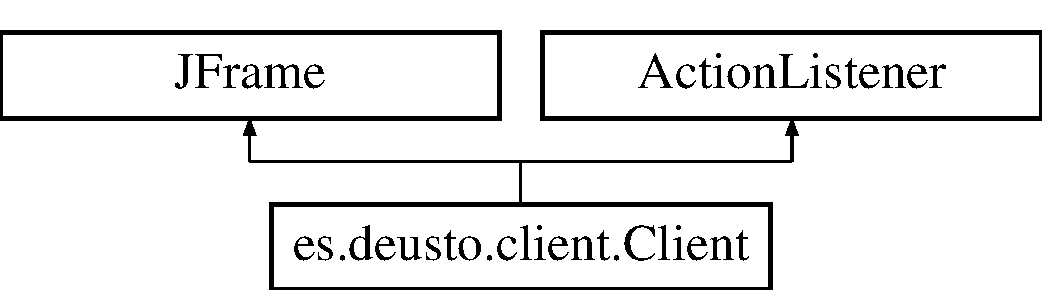
\includegraphics[height=2.000000cm]{classes_1_1deusto_1_1client_1_1_client}
\end{center}
\end{figure}
\subsection*{Public Member Functions}
\begin{DoxyCompactItemize}
\item 
\hyperlink{classes_1_1deusto_1_1client_1_1_client_a71c03e318a72447da873297f3364f67f}{Client} ()
\item 
void \hyperlink{classes_1_1deusto_1_1client_1_1_client_a57eb7a5154b4b1559430f90a1c1df852}{action\+Performed} (Action\+Event e)
\item 
void \hyperlink{classes_1_1deusto_1_1client_1_1_client_a141b9b15a5ba7dc5b3daf2032529575f}{rellenar\+Tabla\+Prod} (Array\+List$<$ \hyperlink{classes_1_1deusto_1_1server_1_1db_1_1data_1_1_product}{Product} $>$ p\+List)
\item 
void \hyperlink{classes_1_1deusto_1_1client_1_1_client_a8c6076e43a37a66a27a00f458eeab3de}{rellenar\+Tabla\+User} (Array\+List$<$ \hyperlink{classes_1_1deusto_1_1server_1_1db_1_1data_1_1_user}{User} $>$ u\+List)
\end{DoxyCompactItemize}
\subsection*{Static Public Member Functions}
\begin{DoxyCompactItemize}
\item 
static void \hyperlink{classes_1_1deusto_1_1client_1_1_client_a69a7526d0af9cb2341f4bf341b501152}{main} (String\mbox{[}$\,$\mbox{]} args)
\end{DoxyCompactItemize}


\subsection{Detailed Description}


Definition at line 29 of file Client.\+java.



\subsection{Constructor \& Destructor Documentation}
\mbox{\Hypertarget{classes_1_1deusto_1_1client_1_1_client_a71c03e318a72447da873297f3364f67f}\label{classes_1_1deusto_1_1client_1_1_client_a71c03e318a72447da873297f3364f67f}} 
\index{es\+::deusto\+::client\+::\+Client@{es\+::deusto\+::client\+::\+Client}!Client@{Client}}
\index{Client@{Client}!es\+::deusto\+::client\+::\+Client@{es\+::deusto\+::client\+::\+Client}}
\subsubsection{\texorpdfstring{Client()}{Client()}}
{\footnotesize\ttfamily es.\+deusto.\+client.\+Client.\+Client (\begin{DoxyParamCaption}{ }\end{DoxyParamCaption})}

Generates a \hyperlink{classes_1_1deusto_1_1client_1_1_client}{Client} Window with all the different attributes it has, begins with a log in and then allows the user to send money, search a product, insert new products, search for all the users (if it has permission), etc. 

Definition at line 64 of file Client.\+java.



\subsection{Member Function Documentation}
\mbox{\Hypertarget{classes_1_1deusto_1_1client_1_1_client_a57eb7a5154b4b1559430f90a1c1df852}\label{classes_1_1deusto_1_1client_1_1_client_a57eb7a5154b4b1559430f90a1c1df852}} 
\index{es\+::deusto\+::client\+::\+Client@{es\+::deusto\+::client\+::\+Client}!action\+Performed@{action\+Performed}}
\index{action\+Performed@{action\+Performed}!es\+::deusto\+::client\+::\+Client@{es\+::deusto\+::client\+::\+Client}}
\subsubsection{\texorpdfstring{action\+Performed()}{actionPerformed()}}
{\footnotesize\ttfamily void es.\+deusto.\+client.\+Client.\+action\+Performed (\begin{DoxyParamCaption}\item[{Action\+Event}]{e }\end{DoxyParamCaption})}



Definition at line 225 of file Client.\+java.

\mbox{\Hypertarget{classes_1_1deusto_1_1client_1_1_client_a69a7526d0af9cb2341f4bf341b501152}\label{classes_1_1deusto_1_1client_1_1_client_a69a7526d0af9cb2341f4bf341b501152}} 
\index{es\+::deusto\+::client\+::\+Client@{es\+::deusto\+::client\+::\+Client}!main@{main}}
\index{main@{main}!es\+::deusto\+::client\+::\+Client@{es\+::deusto\+::client\+::\+Client}}
\subsubsection{\texorpdfstring{main()}{main()}}
{\footnotesize\ttfamily static void es.\+deusto.\+client.\+Client.\+main (\begin{DoxyParamCaption}\item[{String \mbox{[}$\,$\mbox{]}}]{args }\end{DoxyParamCaption})\hspace{0.3cm}{\ttfamily [static]}}



Definition at line 201 of file Client.\+java.

\mbox{\Hypertarget{classes_1_1deusto_1_1client_1_1_client_a141b9b15a5ba7dc5b3daf2032529575f}\label{classes_1_1deusto_1_1client_1_1_client_a141b9b15a5ba7dc5b3daf2032529575f}} 
\index{es\+::deusto\+::client\+::\+Client@{es\+::deusto\+::client\+::\+Client}!rellenar\+Tabla\+Prod@{rellenar\+Tabla\+Prod}}
\index{rellenar\+Tabla\+Prod@{rellenar\+Tabla\+Prod}!es\+::deusto\+::client\+::\+Client@{es\+::deusto\+::client\+::\+Client}}
\subsubsection{\texorpdfstring{rellenar\+Tabla\+Prod()}{rellenarTablaProd()}}
{\footnotesize\ttfamily void es.\+deusto.\+client.\+Client.\+rellenar\+Tabla\+Prod (\begin{DoxyParamCaption}\item[{Array\+List$<$ \hyperlink{classes_1_1deusto_1_1server_1_1db_1_1data_1_1_product}{Product} $>$}]{p\+List }\end{DoxyParamCaption})}

Fill the table (this.\+table) with the Array\+List set by parameter after switching the title of the second column to \char`\"{}\+Description\char`\"{} 
\begin{DoxyParams}{Parameters}
{\em p\+List} & The list of all the products inside the DB \\
\hline
\end{DoxyParams}


Definition at line 334 of file Client.\+java.

\mbox{\Hypertarget{classes_1_1deusto_1_1client_1_1_client_a8c6076e43a37a66a27a00f458eeab3de}\label{classes_1_1deusto_1_1client_1_1_client_a8c6076e43a37a66a27a00f458eeab3de}} 
\index{es\+::deusto\+::client\+::\+Client@{es\+::deusto\+::client\+::\+Client}!rellenar\+Tabla\+User@{rellenar\+Tabla\+User}}
\index{rellenar\+Tabla\+User@{rellenar\+Tabla\+User}!es\+::deusto\+::client\+::\+Client@{es\+::deusto\+::client\+::\+Client}}
\subsubsection{\texorpdfstring{rellenar\+Tabla\+User()}{rellenarTablaUser()}}
{\footnotesize\ttfamily void es.\+deusto.\+client.\+Client.\+rellenar\+Tabla\+User (\begin{DoxyParamCaption}\item[{Array\+List$<$ \hyperlink{classes_1_1deusto_1_1server_1_1db_1_1data_1_1_user}{User} $>$}]{u\+List }\end{DoxyParamCaption})}

Fill the table (this.\+table) with the Array\+List set by parameter after switching the title of the second column to \char`\"{}\+Password\char`\"{} 
\begin{DoxyParams}{Parameters}
{\em u\+List} & The list of all the users inside the DB \\
\hline
\end{DoxyParams}


Definition at line 356 of file Client.\+java.



The documentation for this class was generated from the following file\+:\begin{DoxyCompactItemize}
\item 
C\+:/\+Users/\+Oihane/git/\+S\+P\+Q03/spq03/src/main/java/es/deusto/client/\hyperlink{_client_8java}{Client.\+java}\end{DoxyCompactItemize}

\hypertarget{classes_1_1deusto_1_1server_1_1db_1_1dao_1_1_d_a_o}{}\section{es.\+deusto.\+server.\+db.\+dao.\+D\+AO Class Reference}
\label{classes_1_1deusto_1_1server_1_1db_1_1dao_1_1_d_a_o}\index{es.\+deusto.\+server.\+db.\+dao.\+D\+AO@{es.\+deusto.\+server.\+db.\+dao.\+D\+AO}}
Inheritance diagram for es.\+deusto.\+server.\+db.\+dao.\+D\+AO\+:\begin{figure}[H]
\begin{center}
\leavevmode
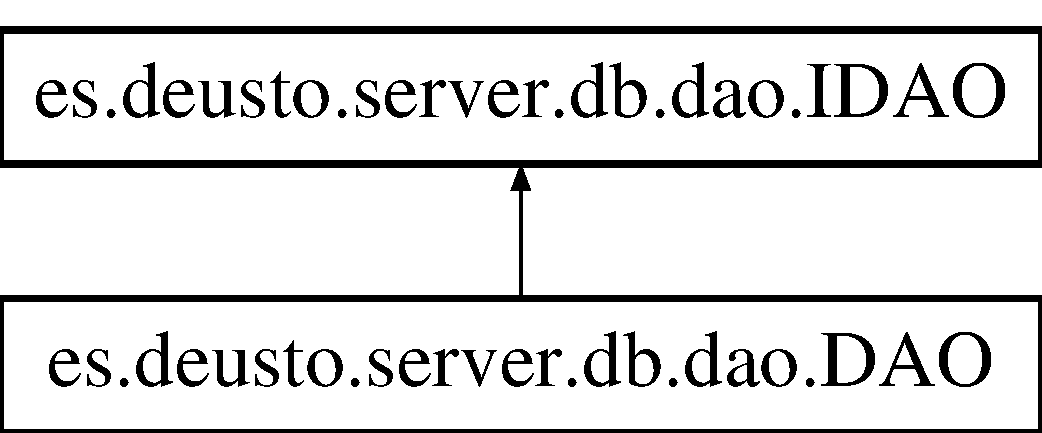
\includegraphics[height=2.000000cm]{classes_1_1deusto_1_1server_1_1db_1_1dao_1_1_d_a_o}
\end{center}
\end{figure}
\subsection*{Public Member Functions}
\begin{DoxyCompactItemize}
\item 
\hyperlink{classes_1_1deusto_1_1server_1_1db_1_1dao_1_1_d_a_o_a1f12a4ca454651d41896e45c42db8f90}{D\+AO} ()
\item 
boolean \hyperlink{classes_1_1deusto_1_1server_1_1db_1_1dao_1_1_d_a_o_acb146e96959c340ef828ef8e36b4283c}{store\+User} (\hyperlink{classes_1_1deusto_1_1server_1_1db_1_1data_1_1_user}{User} u)
\item 
List$<$ \hyperlink{classes_1_1deusto_1_1server_1_1db_1_1data_1_1_user}{User} $>$ \hyperlink{classes_1_1deusto_1_1server_1_1db_1_1dao_1_1_d_a_o_a0ee6fd52276091b7e40129d1c484ef14}{get\+All\+User} ()
\item 
\hyperlink{classes_1_1deusto_1_1server_1_1db_1_1data_1_1_user}{User} \hyperlink{classes_1_1deusto_1_1server_1_1db_1_1dao_1_1_d_a_o_a8c316b4c3bf246d00fb2b423a603ebe6}{retrieve\+User} (String login)
\item 
boolean \hyperlink{classes_1_1deusto_1_1server_1_1db_1_1dao_1_1_d_a_o_a7f6ed77294fe1f61cbebbea410cef6e0}{update\+User} (\hyperlink{classes_1_1deusto_1_1server_1_1db_1_1data_1_1_user}{User} u)
\item 
boolean \hyperlink{classes_1_1deusto_1_1server_1_1db_1_1dao_1_1_d_a_o_a345f30d95426e1cc8bd845949978dd1c}{store\+Prod} (\hyperlink{classes_1_1deusto_1_1server_1_1db_1_1data_1_1_product}{Product} p)
\item 
List$<$ \hyperlink{classes_1_1deusto_1_1server_1_1db_1_1data_1_1_product}{Product} $>$ \hyperlink{classes_1_1deusto_1_1server_1_1db_1_1dao_1_1_d_a_o_a589bc944971075e694d9dc8eabf76870}{get\+All\+Prod} ()
\item 
\hyperlink{classes_1_1deusto_1_1server_1_1db_1_1data_1_1_product}{Product} \hyperlink{classes_1_1deusto_1_1server_1_1db_1_1dao_1_1_d_a_o_a5b4aa30073fdf9ea4263a86165ed4c18}{retrieve\+Prod\+Search} (String name)
\item 
boolean \hyperlink{classes_1_1deusto_1_1server_1_1db_1_1dao_1_1_d_a_o_a2a7817f0def3d19a7871910ebba76df7}{update\+Prod} (\hyperlink{classes_1_1deusto_1_1server_1_1db_1_1data_1_1_product}{Product} p)
\item 
boolean \hyperlink{classes_1_1deusto_1_1server_1_1db_1_1dao_1_1_d_a_o_a0cfb218b648ebc99aed950614173b6c6}{store\+Money} (\hyperlink{classes_1_1deusto_1_1server_1_1db_1_1data_1_1_money}{Money} m)
\item 
\hyperlink{classes_1_1deusto_1_1server_1_1db_1_1data_1_1_money}{Money} \hyperlink{classes_1_1deusto_1_1server_1_1db_1_1dao_1_1_d_a_o_a171a709ad2008e5eea8a77db494df1d0}{retrieve\+Money} (int amount)
\item 
boolean \hyperlink{classes_1_1deusto_1_1server_1_1db_1_1dao_1_1_d_a_o_a05c7fc41d49e5ab7f0830405ccf60c87}{update\+Money} (\hyperlink{classes_1_1deusto_1_1server_1_1db_1_1data_1_1_money}{Money} m)
\end{DoxyCompactItemize}


\subsection{Detailed Description}


Definition at line 12 of file D\+A\+O.\+java.



\subsection{Constructor \& Destructor Documentation}
\mbox{\Hypertarget{classes_1_1deusto_1_1server_1_1db_1_1dao_1_1_d_a_o_a1f12a4ca454651d41896e45c42db8f90}\label{classes_1_1deusto_1_1server_1_1db_1_1dao_1_1_d_a_o_a1f12a4ca454651d41896e45c42db8f90}} 
\index{es\+::deusto\+::server\+::db\+::dao\+::\+D\+AO@{es\+::deusto\+::server\+::db\+::dao\+::\+D\+AO}!D\+AO@{D\+AO}}
\index{D\+AO@{D\+AO}!es\+::deusto\+::server\+::db\+::dao\+::\+D\+AO@{es\+::deusto\+::server\+::db\+::dao\+::\+D\+AO}}
\subsubsection{\texorpdfstring{D\+A\+O()}{DAO()}}
{\footnotesize\ttfamily es.\+deusto.\+server.\+db.\+dao.\+D\+A\+O.\+D\+AO (\begin{DoxyParamCaption}{ }\end{DoxyParamCaption})}



Definition at line 16 of file D\+A\+O.\+java.



\subsection{Member Function Documentation}
\mbox{\Hypertarget{classes_1_1deusto_1_1server_1_1db_1_1dao_1_1_d_a_o_a589bc944971075e694d9dc8eabf76870}\label{classes_1_1deusto_1_1server_1_1db_1_1dao_1_1_d_a_o_a589bc944971075e694d9dc8eabf76870}} 
\index{es\+::deusto\+::server\+::db\+::dao\+::\+D\+AO@{es\+::deusto\+::server\+::db\+::dao\+::\+D\+AO}!get\+All\+Prod@{get\+All\+Prod}}
\index{get\+All\+Prod@{get\+All\+Prod}!es\+::deusto\+::server\+::db\+::dao\+::\+D\+AO@{es\+::deusto\+::server\+::db\+::dao\+::\+D\+AO}}
\subsubsection{\texorpdfstring{get\+All\+Prod()}{getAllProd()}}
{\footnotesize\ttfamily List$<$\hyperlink{classes_1_1deusto_1_1server_1_1db_1_1data_1_1_product}{Product}$>$ es.\+deusto.\+server.\+db.\+dao.\+D\+A\+O.\+get\+All\+Prod (\begin{DoxyParamCaption}{ }\end{DoxyParamCaption})}



Implements \hyperlink{interfacees_1_1deusto_1_1server_1_1db_1_1dao_1_1_i_d_a_o_a5a3e4739557f0af9060b4ca90e69c0e3}{es.\+deusto.\+server.\+db.\+dao.\+I\+D\+AO}.



Definition at line 151 of file D\+A\+O.\+java.

\mbox{\Hypertarget{classes_1_1deusto_1_1server_1_1db_1_1dao_1_1_d_a_o_a0ee6fd52276091b7e40129d1c484ef14}\label{classes_1_1deusto_1_1server_1_1db_1_1dao_1_1_d_a_o_a0ee6fd52276091b7e40129d1c484ef14}} 
\index{es\+::deusto\+::server\+::db\+::dao\+::\+D\+AO@{es\+::deusto\+::server\+::db\+::dao\+::\+D\+AO}!get\+All\+User@{get\+All\+User}}
\index{get\+All\+User@{get\+All\+User}!es\+::deusto\+::server\+::db\+::dao\+::\+D\+AO@{es\+::deusto\+::server\+::db\+::dao\+::\+D\+AO}}
\subsubsection{\texorpdfstring{get\+All\+User()}{getAllUser()}}
{\footnotesize\ttfamily List$<$\hyperlink{classes_1_1deusto_1_1server_1_1db_1_1data_1_1_user}{User}$>$ es.\+deusto.\+server.\+db.\+dao.\+D\+A\+O.\+get\+All\+User (\begin{DoxyParamCaption}{ }\end{DoxyParamCaption})}



Implements \hyperlink{interfacees_1_1deusto_1_1server_1_1db_1_1dao_1_1_i_d_a_o_affa6fc846698427199cb7305155a95c7}{es.\+deusto.\+server.\+db.\+dao.\+I\+D\+AO}.



Definition at line 46 of file D\+A\+O.\+java.

\mbox{\Hypertarget{classes_1_1deusto_1_1server_1_1db_1_1dao_1_1_d_a_o_a171a709ad2008e5eea8a77db494df1d0}\label{classes_1_1deusto_1_1server_1_1db_1_1dao_1_1_d_a_o_a171a709ad2008e5eea8a77db494df1d0}} 
\index{es\+::deusto\+::server\+::db\+::dao\+::\+D\+AO@{es\+::deusto\+::server\+::db\+::dao\+::\+D\+AO}!retrieve\+Money@{retrieve\+Money}}
\index{retrieve\+Money@{retrieve\+Money}!es\+::deusto\+::server\+::db\+::dao\+::\+D\+AO@{es\+::deusto\+::server\+::db\+::dao\+::\+D\+AO}}
\subsubsection{\texorpdfstring{retrieve\+Money()}{retrieveMoney()}}
{\footnotesize\ttfamily \hyperlink{classes_1_1deusto_1_1server_1_1db_1_1data_1_1_money}{Money} es.\+deusto.\+server.\+db.\+dao.\+D\+A\+O.\+retrieve\+Money (\begin{DoxyParamCaption}\item[{int}]{amount }\end{DoxyParamCaption})}



Implements \hyperlink{interfacees_1_1deusto_1_1server_1_1db_1_1dao_1_1_i_d_a_o_a1386c2e329277fc36575b0450a0e8997}{es.\+deusto.\+server.\+db.\+dao.\+I\+D\+AO}.



Definition at line 254 of file D\+A\+O.\+java.

\mbox{\Hypertarget{classes_1_1deusto_1_1server_1_1db_1_1dao_1_1_d_a_o_a5b4aa30073fdf9ea4263a86165ed4c18}\label{classes_1_1deusto_1_1server_1_1db_1_1dao_1_1_d_a_o_a5b4aa30073fdf9ea4263a86165ed4c18}} 
\index{es\+::deusto\+::server\+::db\+::dao\+::\+D\+AO@{es\+::deusto\+::server\+::db\+::dao\+::\+D\+AO}!retrieve\+Prod\+Search@{retrieve\+Prod\+Search}}
\index{retrieve\+Prod\+Search@{retrieve\+Prod\+Search}!es\+::deusto\+::server\+::db\+::dao\+::\+D\+AO@{es\+::deusto\+::server\+::db\+::dao\+::\+D\+AO}}
\subsubsection{\texorpdfstring{retrieve\+Prod\+Search()}{retrieveProdSearch()}}
{\footnotesize\ttfamily \hyperlink{classes_1_1deusto_1_1server_1_1db_1_1data_1_1_product}{Product} es.\+deusto.\+server.\+db.\+dao.\+D\+A\+O.\+retrieve\+Prod\+Search (\begin{DoxyParamCaption}\item[{String}]{name }\end{DoxyParamCaption})}



Implements \hyperlink{interfacees_1_1deusto_1_1server_1_1db_1_1dao_1_1_i_d_a_o_a9ba3fce5b0679bb1068484734fe0ed02}{es.\+deusto.\+server.\+db.\+dao.\+I\+D\+AO}.



Definition at line 181 of file D\+A\+O.\+java.

\mbox{\Hypertarget{classes_1_1deusto_1_1server_1_1db_1_1dao_1_1_d_a_o_a8c316b4c3bf246d00fb2b423a603ebe6}\label{classes_1_1deusto_1_1server_1_1db_1_1dao_1_1_d_a_o_a8c316b4c3bf246d00fb2b423a603ebe6}} 
\index{es\+::deusto\+::server\+::db\+::dao\+::\+D\+AO@{es\+::deusto\+::server\+::db\+::dao\+::\+D\+AO}!retrieve\+User@{retrieve\+User}}
\index{retrieve\+User@{retrieve\+User}!es\+::deusto\+::server\+::db\+::dao\+::\+D\+AO@{es\+::deusto\+::server\+::db\+::dao\+::\+D\+AO}}
\subsubsection{\texorpdfstring{retrieve\+User()}{retrieveUser()}}
{\footnotesize\ttfamily \hyperlink{classes_1_1deusto_1_1server_1_1db_1_1data_1_1_user}{User} es.\+deusto.\+server.\+db.\+dao.\+D\+A\+O.\+retrieve\+User (\begin{DoxyParamCaption}\item[{String}]{login }\end{DoxyParamCaption})}



Implements \hyperlink{interfacees_1_1deusto_1_1server_1_1db_1_1dao_1_1_i_d_a_o_a19f9b0d0b6f5f80730d6d197deca7dfc}{es.\+deusto.\+server.\+db.\+dao.\+I\+D\+AO}.



Definition at line 79 of file D\+A\+O.\+java.

\mbox{\Hypertarget{classes_1_1deusto_1_1server_1_1db_1_1dao_1_1_d_a_o_a0cfb218b648ebc99aed950614173b6c6}\label{classes_1_1deusto_1_1server_1_1db_1_1dao_1_1_d_a_o_a0cfb218b648ebc99aed950614173b6c6}} 
\index{es\+::deusto\+::server\+::db\+::dao\+::\+D\+AO@{es\+::deusto\+::server\+::db\+::dao\+::\+D\+AO}!store\+Money@{store\+Money}}
\index{store\+Money@{store\+Money}!es\+::deusto\+::server\+::db\+::dao\+::\+D\+AO@{es\+::deusto\+::server\+::db\+::dao\+::\+D\+AO}}
\subsubsection{\texorpdfstring{store\+Money()}{storeMoney()}}
{\footnotesize\ttfamily boolean es.\+deusto.\+server.\+db.\+dao.\+D\+A\+O.\+store\+Money (\begin{DoxyParamCaption}\item[{\hyperlink{classes_1_1deusto_1_1server_1_1db_1_1data_1_1_money}{Money}}]{m }\end{DoxyParamCaption})}



Implements \hyperlink{interfacees_1_1deusto_1_1server_1_1db_1_1dao_1_1_i_d_a_o_a0c952a7cac366a448451d8150a8d57e4}{es.\+deusto.\+server.\+db.\+dao.\+I\+D\+AO}.



Definition at line 230 of file D\+A\+O.\+java.

\mbox{\Hypertarget{classes_1_1deusto_1_1server_1_1db_1_1dao_1_1_d_a_o_a345f30d95426e1cc8bd845949978dd1c}\label{classes_1_1deusto_1_1server_1_1db_1_1dao_1_1_d_a_o_a345f30d95426e1cc8bd845949978dd1c}} 
\index{es\+::deusto\+::server\+::db\+::dao\+::\+D\+AO@{es\+::deusto\+::server\+::db\+::dao\+::\+D\+AO}!store\+Prod@{store\+Prod}}
\index{store\+Prod@{store\+Prod}!es\+::deusto\+::server\+::db\+::dao\+::\+D\+AO@{es\+::deusto\+::server\+::db\+::dao\+::\+D\+AO}}
\subsubsection{\texorpdfstring{store\+Prod()}{storeProd()}}
{\footnotesize\ttfamily boolean es.\+deusto.\+server.\+db.\+dao.\+D\+A\+O.\+store\+Prod (\begin{DoxyParamCaption}\item[{\hyperlink{classes_1_1deusto_1_1server_1_1db_1_1data_1_1_product}{Product}}]{p }\end{DoxyParamCaption})}



Implements \hyperlink{interfacees_1_1deusto_1_1server_1_1db_1_1dao_1_1_i_d_a_o_a1f6d1e58c88fb3a24021f94de5e70056}{es.\+deusto.\+server.\+db.\+dao.\+I\+D\+AO}.



Definition at line 128 of file D\+A\+O.\+java.

\mbox{\Hypertarget{classes_1_1deusto_1_1server_1_1db_1_1dao_1_1_d_a_o_acb146e96959c340ef828ef8e36b4283c}\label{classes_1_1deusto_1_1server_1_1db_1_1dao_1_1_d_a_o_acb146e96959c340ef828ef8e36b4283c}} 
\index{es\+::deusto\+::server\+::db\+::dao\+::\+D\+AO@{es\+::deusto\+::server\+::db\+::dao\+::\+D\+AO}!store\+User@{store\+User}}
\index{store\+User@{store\+User}!es\+::deusto\+::server\+::db\+::dao\+::\+D\+AO@{es\+::deusto\+::server\+::db\+::dao\+::\+D\+AO}}
\subsubsection{\texorpdfstring{store\+User()}{storeUser()}}
{\footnotesize\ttfamily boolean es.\+deusto.\+server.\+db.\+dao.\+D\+A\+O.\+store\+User (\begin{DoxyParamCaption}\item[{\hyperlink{classes_1_1deusto_1_1server_1_1db_1_1data_1_1_user}{User}}]{u }\end{DoxyParamCaption})}



Implements \hyperlink{interfacees_1_1deusto_1_1server_1_1db_1_1dao_1_1_i_d_a_o_ab943216560f43595a852b406dcd394a4}{es.\+deusto.\+server.\+db.\+dao.\+I\+D\+AO}.



Definition at line 21 of file D\+A\+O.\+java.

\mbox{\Hypertarget{classes_1_1deusto_1_1server_1_1db_1_1dao_1_1_d_a_o_a05c7fc41d49e5ab7f0830405ccf60c87}\label{classes_1_1deusto_1_1server_1_1db_1_1dao_1_1_d_a_o_a05c7fc41d49e5ab7f0830405ccf60c87}} 
\index{es\+::deusto\+::server\+::db\+::dao\+::\+D\+AO@{es\+::deusto\+::server\+::db\+::dao\+::\+D\+AO}!update\+Money@{update\+Money}}
\index{update\+Money@{update\+Money}!es\+::deusto\+::server\+::db\+::dao\+::\+D\+AO@{es\+::deusto\+::server\+::db\+::dao\+::\+D\+AO}}
\subsubsection{\texorpdfstring{update\+Money()}{updateMoney()}}
{\footnotesize\ttfamily boolean es.\+deusto.\+server.\+db.\+dao.\+D\+A\+O.\+update\+Money (\begin{DoxyParamCaption}\item[{\hyperlink{classes_1_1deusto_1_1server_1_1db_1_1data_1_1_money}{Money}}]{m }\end{DoxyParamCaption})}



Implements \hyperlink{interfacees_1_1deusto_1_1server_1_1db_1_1dao_1_1_i_d_a_o_a2a4641aeefc28dc979e0146e8ca73342}{es.\+deusto.\+server.\+db.\+dao.\+I\+D\+AO}.



Definition at line 279 of file D\+A\+O.\+java.

\mbox{\Hypertarget{classes_1_1deusto_1_1server_1_1db_1_1dao_1_1_d_a_o_a2a7817f0def3d19a7871910ebba76df7}\label{classes_1_1deusto_1_1server_1_1db_1_1dao_1_1_d_a_o_a2a7817f0def3d19a7871910ebba76df7}} 
\index{es\+::deusto\+::server\+::db\+::dao\+::\+D\+AO@{es\+::deusto\+::server\+::db\+::dao\+::\+D\+AO}!update\+Prod@{update\+Prod}}
\index{update\+Prod@{update\+Prod}!es\+::deusto\+::server\+::db\+::dao\+::\+D\+AO@{es\+::deusto\+::server\+::db\+::dao\+::\+D\+AO}}
\subsubsection{\texorpdfstring{update\+Prod()}{updateProd()}}
{\footnotesize\ttfamily boolean es.\+deusto.\+server.\+db.\+dao.\+D\+A\+O.\+update\+Prod (\begin{DoxyParamCaption}\item[{\hyperlink{classes_1_1deusto_1_1server_1_1db_1_1data_1_1_product}{Product}}]{p }\end{DoxyParamCaption})}



Implements \hyperlink{interfacees_1_1deusto_1_1server_1_1db_1_1dao_1_1_i_d_a_o_afc4634e403796a1b66fc5251b5b86d1e}{es.\+deusto.\+server.\+db.\+dao.\+I\+D\+AO}.



Definition at line 208 of file D\+A\+O.\+java.

\mbox{\Hypertarget{classes_1_1deusto_1_1server_1_1db_1_1dao_1_1_d_a_o_a7f6ed77294fe1f61cbebbea410cef6e0}\label{classes_1_1deusto_1_1server_1_1db_1_1dao_1_1_d_a_o_a7f6ed77294fe1f61cbebbea410cef6e0}} 
\index{es\+::deusto\+::server\+::db\+::dao\+::\+D\+AO@{es\+::deusto\+::server\+::db\+::dao\+::\+D\+AO}!update\+User@{update\+User}}
\index{update\+User@{update\+User}!es\+::deusto\+::server\+::db\+::dao\+::\+D\+AO@{es\+::deusto\+::server\+::db\+::dao\+::\+D\+AO}}
\subsubsection{\texorpdfstring{update\+User()}{updateUser()}}
{\footnotesize\ttfamily boolean es.\+deusto.\+server.\+db.\+dao.\+D\+A\+O.\+update\+User (\begin{DoxyParamCaption}\item[{\hyperlink{classes_1_1deusto_1_1server_1_1db_1_1data_1_1_user}{User}}]{u }\end{DoxyParamCaption})}



Implements \hyperlink{interfacees_1_1deusto_1_1server_1_1db_1_1dao_1_1_i_d_a_o_a790b00e2989b634c1bbb2c6620ff3583}{es.\+deusto.\+server.\+db.\+dao.\+I\+D\+AO}.



Definition at line 105 of file D\+A\+O.\+java.



The documentation for this class was generated from the following file\+:\begin{DoxyCompactItemize}
\item 
C\+:/\+Users/\+Oihane/git/\+S\+P\+Q03/spq03/src/main/java/es/deusto/server/db/dao/\hyperlink{_d_a_o_8java}{D\+A\+O.\+java}\end{DoxyCompactItemize}

\hypertarget{classes_1_1deusto_1_1server_1_1db_1_1_d_b}{}\section{es.\+deusto.\+server.\+db.\+DB Class Reference}
\label{classes_1_1deusto_1_1server_1_1db_1_1_d_b}\index{es.\+deusto.\+server.\+db.\+DB@{es.\+deusto.\+server.\+db.\+DB}}
Inheritance diagram for es.\+deusto.\+server.\+db.\+DB\+:\begin{figure}[H]
\begin{center}
\leavevmode
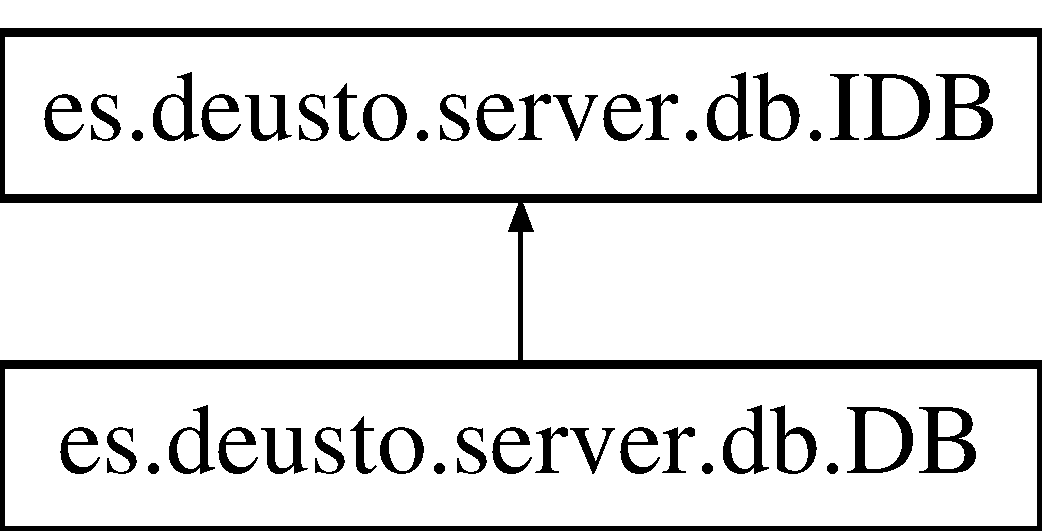
\includegraphics[height=2.000000cm]{classes_1_1deusto_1_1server_1_1db_1_1_d_b}
\end{center}
\end{figure}
\subsection*{Public Member Functions}
\begin{DoxyCompactItemize}
\item 
\hyperlink{classes_1_1deusto_1_1server_1_1db_1_1_d_b_ab53f32f36928ba9aa3ddff65fce395dc}{DB} ()
\item 
\hyperlink{classes_1_1deusto_1_1server_1_1db_1_1_d_b_a8c85804ab042af947fd1a749ff42fd0d}{DB} (\hyperlink{interfacees_1_1deusto_1_1server_1_1db_1_1dao_1_1_i_d_a_o}{I\+D\+AO} idao)
\item 
List$<$ \hyperlink{classes_1_1deusto_1_1server_1_1db_1_1data_1_1_product}{Product} $>$ \hyperlink{classes_1_1deusto_1_1server_1_1db_1_1_d_b_aa193a59efe6c2458d89fd751da935a3a}{get\+All\+Prod} ()
\item 
\hyperlink{classes_1_1deusto_1_1server_1_1db_1_1data_1_1_product}{Product} \hyperlink{classes_1_1deusto_1_1server_1_1db_1_1_d_b_a1c170a7c91ca5223560b4490738ccf56}{show\+Prod} (String name)
\item 
\hyperlink{classes_1_1deusto_1_1server_1_1db_1_1data_1_1_user}{User} \hyperlink{classes_1_1deusto_1_1server_1_1db_1_1_d_b_ac85523faea523033439a932bbcab2c7e}{show\+User} (String login)
\item 
boolean \hyperlink{classes_1_1deusto_1_1server_1_1db_1_1_d_b_a2f5a50ff22834658b641ebf6bb7afbe6}{insert\+Prod} (\hyperlink{classes_1_1deusto_1_1server_1_1db_1_1data_1_1_product}{Product} p)
\item 
boolean \hyperlink{classes_1_1deusto_1_1server_1_1db_1_1_d_b_a1070e289debd4f0fb5519c245c4e7ed7}{insert\+User} (\hyperlink{classes_1_1deusto_1_1server_1_1db_1_1data_1_1_user}{User} u)
\item 
boolean \hyperlink{classes_1_1deusto_1_1server_1_1db_1_1_d_b_ab9a9acacfc8dadaeec7159c0886dfec2}{insert\+Money} (\hyperlink{classes_1_1deusto_1_1server_1_1db_1_1data_1_1_money}{Money} m)
\item 
boolean \hyperlink{classes_1_1deusto_1_1server_1_1db_1_1_d_b_a06ce3aee905784e5ec88a8945452548e}{buy\+Prod} (String loginB, String loginS, String name, int amount)
\end{DoxyCompactItemize}


\subsection{Detailed Description}


Definition at line 16 of file D\+B.\+java.



\subsection{Constructor \& Destructor Documentation}
\mbox{\Hypertarget{classes_1_1deusto_1_1server_1_1db_1_1_d_b_ab53f32f36928ba9aa3ddff65fce395dc}\label{classes_1_1deusto_1_1server_1_1db_1_1_d_b_ab53f32f36928ba9aa3ddff65fce395dc}} 
\index{es\+::deusto\+::server\+::db\+::\+DB@{es\+::deusto\+::server\+::db\+::\+DB}!DB@{DB}}
\index{DB@{DB}!es\+::deusto\+::server\+::db\+::\+DB@{es\+::deusto\+::server\+::db\+::\+DB}}
\subsubsection{\texorpdfstring{D\+B()}{DB()}\hspace{0.1cm}{\footnotesize\ttfamily [1/2]}}
{\footnotesize\ttfamily es.\+deusto.\+server.\+db.\+D\+B.\+DB (\begin{DoxyParamCaption}{ }\end{DoxyParamCaption})}



Definition at line 23 of file D\+B.\+java.

\mbox{\Hypertarget{classes_1_1deusto_1_1server_1_1db_1_1_d_b_a8c85804ab042af947fd1a749ff42fd0d}\label{classes_1_1deusto_1_1server_1_1db_1_1_d_b_a8c85804ab042af947fd1a749ff42fd0d}} 
\index{es\+::deusto\+::server\+::db\+::\+DB@{es\+::deusto\+::server\+::db\+::\+DB}!DB@{DB}}
\index{DB@{DB}!es\+::deusto\+::server\+::db\+::\+DB@{es\+::deusto\+::server\+::db\+::\+DB}}
\subsubsection{\texorpdfstring{D\+B()}{DB()}\hspace{0.1cm}{\footnotesize\ttfamily [2/2]}}
{\footnotesize\ttfamily es.\+deusto.\+server.\+db.\+D\+B.\+DB (\begin{DoxyParamCaption}\item[{\hyperlink{interfacees_1_1deusto_1_1server_1_1db_1_1dao_1_1_i_d_a_o}{I\+D\+AO}}]{idao }\end{DoxyParamCaption})}



Definition at line 28 of file D\+B.\+java.



\subsection{Member Function Documentation}
\mbox{\Hypertarget{classes_1_1deusto_1_1server_1_1db_1_1_d_b_a06ce3aee905784e5ec88a8945452548e}\label{classes_1_1deusto_1_1server_1_1db_1_1_d_b_a06ce3aee905784e5ec88a8945452548e}} 
\index{es\+::deusto\+::server\+::db\+::\+DB@{es\+::deusto\+::server\+::db\+::\+DB}!buy\+Prod@{buy\+Prod}}
\index{buy\+Prod@{buy\+Prod}!es\+::deusto\+::server\+::db\+::\+DB@{es\+::deusto\+::server\+::db\+::\+DB}}
\subsubsection{\texorpdfstring{buy\+Prod()}{buyProd()}}
{\footnotesize\ttfamily boolean es.\+deusto.\+server.\+db.\+D\+B.\+buy\+Prod (\begin{DoxyParamCaption}\item[{String}]{loginB,  }\item[{String}]{loginS,  }\item[{String}]{name,  }\item[{int}]{amount }\end{DoxyParamCaption})}



Implements \hyperlink{interfacees_1_1deusto_1_1server_1_1db_1_1_i_d_b_a64b43ced1334b833f7ee557badd2c5b7}{es.\+deusto.\+server.\+db.\+I\+DB}.



Definition at line 134 of file D\+B.\+java.

\mbox{\Hypertarget{classes_1_1deusto_1_1server_1_1db_1_1_d_b_aa193a59efe6c2458d89fd751da935a3a}\label{classes_1_1deusto_1_1server_1_1db_1_1_d_b_aa193a59efe6c2458d89fd751da935a3a}} 
\index{es\+::deusto\+::server\+::db\+::\+DB@{es\+::deusto\+::server\+::db\+::\+DB}!get\+All\+Prod@{get\+All\+Prod}}
\index{get\+All\+Prod@{get\+All\+Prod}!es\+::deusto\+::server\+::db\+::\+DB@{es\+::deusto\+::server\+::db\+::\+DB}}
\subsubsection{\texorpdfstring{get\+All\+Prod()}{getAllProd()}}
{\footnotesize\ttfamily List$<$\hyperlink{classes_1_1deusto_1_1server_1_1db_1_1data_1_1_product}{Product}$>$ es.\+deusto.\+server.\+db.\+D\+B.\+get\+All\+Prod (\begin{DoxyParamCaption}{ }\end{DoxyParamCaption})}



Implements \hyperlink{interfacees_1_1deusto_1_1server_1_1db_1_1_i_d_b_aba694290fde102c2eed31e505dd257fb}{es.\+deusto.\+server.\+db.\+I\+DB}.



Definition at line 34 of file D\+B.\+java.

\mbox{\Hypertarget{classes_1_1deusto_1_1server_1_1db_1_1_d_b_ab9a9acacfc8dadaeec7159c0886dfec2}\label{classes_1_1deusto_1_1server_1_1db_1_1_d_b_ab9a9acacfc8dadaeec7159c0886dfec2}} 
\index{es\+::deusto\+::server\+::db\+::\+DB@{es\+::deusto\+::server\+::db\+::\+DB}!insert\+Money@{insert\+Money}}
\index{insert\+Money@{insert\+Money}!es\+::deusto\+::server\+::db\+::\+DB@{es\+::deusto\+::server\+::db\+::\+DB}}
\subsubsection{\texorpdfstring{insert\+Money()}{insertMoney()}}
{\footnotesize\ttfamily boolean es.\+deusto.\+server.\+db.\+D\+B.\+insert\+Money (\begin{DoxyParamCaption}\item[{\hyperlink{classes_1_1deusto_1_1server_1_1db_1_1data_1_1_money}{Money}}]{m }\end{DoxyParamCaption})}



Implements \hyperlink{interfacees_1_1deusto_1_1server_1_1db_1_1_i_d_b_afcce296d82fa0a6fb8083215b3647663}{es.\+deusto.\+server.\+db.\+I\+DB}.



Definition at line 113 of file D\+B.\+java.

\mbox{\Hypertarget{classes_1_1deusto_1_1server_1_1db_1_1_d_b_a2f5a50ff22834658b641ebf6bb7afbe6}\label{classes_1_1deusto_1_1server_1_1db_1_1_d_b_a2f5a50ff22834658b641ebf6bb7afbe6}} 
\index{es\+::deusto\+::server\+::db\+::\+DB@{es\+::deusto\+::server\+::db\+::\+DB}!insert\+Prod@{insert\+Prod}}
\index{insert\+Prod@{insert\+Prod}!es\+::deusto\+::server\+::db\+::\+DB@{es\+::deusto\+::server\+::db\+::\+DB}}
\subsubsection{\texorpdfstring{insert\+Prod()}{insertProd()}}
{\footnotesize\ttfamily boolean es.\+deusto.\+server.\+db.\+D\+B.\+insert\+Prod (\begin{DoxyParamCaption}\item[{\hyperlink{classes_1_1deusto_1_1server_1_1db_1_1data_1_1_product}{Product}}]{p }\end{DoxyParamCaption})}



Implements \hyperlink{interfacees_1_1deusto_1_1server_1_1db_1_1_i_d_b_a4c9c0a9511fde5b541a49de8f8399d28}{es.\+deusto.\+server.\+db.\+I\+DB}.



Definition at line 67 of file D\+B.\+java.

\mbox{\Hypertarget{classes_1_1deusto_1_1server_1_1db_1_1_d_b_a1070e289debd4f0fb5519c245c4e7ed7}\label{classes_1_1deusto_1_1server_1_1db_1_1_d_b_a1070e289debd4f0fb5519c245c4e7ed7}} 
\index{es\+::deusto\+::server\+::db\+::\+DB@{es\+::deusto\+::server\+::db\+::\+DB}!insert\+User@{insert\+User}}
\index{insert\+User@{insert\+User}!es\+::deusto\+::server\+::db\+::\+DB@{es\+::deusto\+::server\+::db\+::\+DB}}
\subsubsection{\texorpdfstring{insert\+User()}{insertUser()}}
{\footnotesize\ttfamily boolean es.\+deusto.\+server.\+db.\+D\+B.\+insert\+User (\begin{DoxyParamCaption}\item[{\hyperlink{classes_1_1deusto_1_1server_1_1db_1_1data_1_1_user}{User}}]{u }\end{DoxyParamCaption})}



Implements \hyperlink{interfacees_1_1deusto_1_1server_1_1db_1_1_i_d_b_a9d76b65686526214b48cd7d8f8dcdc86}{es.\+deusto.\+server.\+db.\+I\+DB}.



Definition at line 90 of file D\+B.\+java.

\mbox{\Hypertarget{classes_1_1deusto_1_1server_1_1db_1_1_d_b_a1c170a7c91ca5223560b4490738ccf56}\label{classes_1_1deusto_1_1server_1_1db_1_1_d_b_a1c170a7c91ca5223560b4490738ccf56}} 
\index{es\+::deusto\+::server\+::db\+::\+DB@{es\+::deusto\+::server\+::db\+::\+DB}!show\+Prod@{show\+Prod}}
\index{show\+Prod@{show\+Prod}!es\+::deusto\+::server\+::db\+::\+DB@{es\+::deusto\+::server\+::db\+::\+DB}}
\subsubsection{\texorpdfstring{show\+Prod()}{showProd()}}
{\footnotesize\ttfamily \hyperlink{classes_1_1deusto_1_1server_1_1db_1_1data_1_1_product}{Product} es.\+deusto.\+server.\+db.\+D\+B.\+show\+Prod (\begin{DoxyParamCaption}\item[{String}]{name }\end{DoxyParamCaption})}



Implements \hyperlink{interfacees_1_1deusto_1_1server_1_1db_1_1_i_d_b_a8a4f72bb5148aff5b6f82679a7650b29}{es.\+deusto.\+server.\+db.\+I\+DB}.



Definition at line 45 of file D\+B.\+java.

\mbox{\Hypertarget{classes_1_1deusto_1_1server_1_1db_1_1_d_b_ac85523faea523033439a932bbcab2c7e}\label{classes_1_1deusto_1_1server_1_1db_1_1_d_b_ac85523faea523033439a932bbcab2c7e}} 
\index{es\+::deusto\+::server\+::db\+::\+DB@{es\+::deusto\+::server\+::db\+::\+DB}!show\+User@{show\+User}}
\index{show\+User@{show\+User}!es\+::deusto\+::server\+::db\+::\+DB@{es\+::deusto\+::server\+::db\+::\+DB}}
\subsubsection{\texorpdfstring{show\+User()}{showUser()}}
{\footnotesize\ttfamily \hyperlink{classes_1_1deusto_1_1server_1_1db_1_1data_1_1_user}{User} es.\+deusto.\+server.\+db.\+D\+B.\+show\+User (\begin{DoxyParamCaption}\item[{String}]{login }\end{DoxyParamCaption})}



Implements \hyperlink{interfacees_1_1deusto_1_1server_1_1db_1_1_i_d_b_aa2f6a5291fa8aa78d5a73b5878d17986}{es.\+deusto.\+server.\+db.\+I\+DB}.



Definition at line 56 of file D\+B.\+java.



The documentation for this class was generated from the following file\+:\begin{DoxyCompactItemize}
\item 
C\+:/\+Users/\+Oihane/git/\+S\+P\+Q03/spq03/src/main/java/es/deusto/server/db/\hyperlink{_d_b_8java}{D\+B.\+java}\end{DoxyCompactItemize}

\hypertarget{interfacees_1_1deusto_1_1server_1_1db_1_1dao_1_1_i_d_a_o}{}\section{es.\+deusto.\+server.\+db.\+dao.\+I\+D\+AO Interface Reference}
\label{interfacees_1_1deusto_1_1server_1_1db_1_1dao_1_1_i_d_a_o}\index{es.\+deusto.\+server.\+db.\+dao.\+I\+D\+AO@{es.\+deusto.\+server.\+db.\+dao.\+I\+D\+AO}}
Inheritance diagram for es.\+deusto.\+server.\+db.\+dao.\+I\+D\+AO\+:\begin{figure}[H]
\begin{center}
\leavevmode
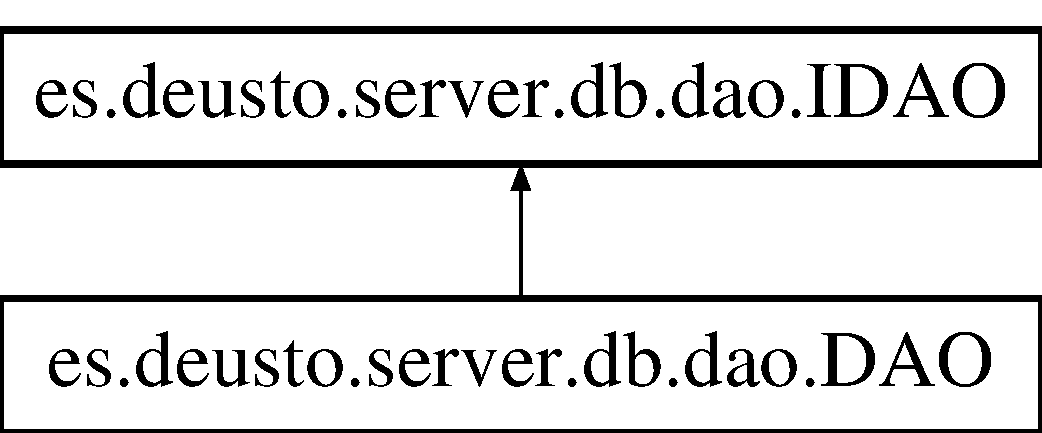
\includegraphics[height=2.000000cm]{interfacees_1_1deusto_1_1server_1_1db_1_1dao_1_1_i_d_a_o}
\end{center}
\end{figure}
\subsection*{Public Member Functions}
\begin{DoxyCompactItemize}
\item 
boolean \hyperlink{interfacees_1_1deusto_1_1server_1_1db_1_1dao_1_1_i_d_a_o_ab943216560f43595a852b406dcd394a4}{store\+User} (\hyperlink{classes_1_1deusto_1_1server_1_1db_1_1data_1_1_user}{User} u)
\item 
List$<$ \hyperlink{classes_1_1deusto_1_1server_1_1db_1_1data_1_1_user}{User} $>$ \hyperlink{interfacees_1_1deusto_1_1server_1_1db_1_1dao_1_1_i_d_a_o_affa6fc846698427199cb7305155a95c7}{get\+All\+User} ()
\item 
\hyperlink{classes_1_1deusto_1_1server_1_1db_1_1data_1_1_user}{User} \hyperlink{interfacees_1_1deusto_1_1server_1_1db_1_1dao_1_1_i_d_a_o_a19f9b0d0b6f5f80730d6d197deca7dfc}{retrieve\+User} (String login)
\item 
boolean \hyperlink{interfacees_1_1deusto_1_1server_1_1db_1_1dao_1_1_i_d_a_o_a790b00e2989b634c1bbb2c6620ff3583}{update\+User} (\hyperlink{classes_1_1deusto_1_1server_1_1db_1_1data_1_1_user}{User} u)
\item 
boolean \hyperlink{interfacees_1_1deusto_1_1server_1_1db_1_1dao_1_1_i_d_a_o_a1f6d1e58c88fb3a24021f94de5e70056}{store\+Prod} (\hyperlink{classes_1_1deusto_1_1server_1_1db_1_1data_1_1_product}{Product} p)
\item 
List$<$ \hyperlink{classes_1_1deusto_1_1server_1_1db_1_1data_1_1_product}{Product} $>$ \hyperlink{interfacees_1_1deusto_1_1server_1_1db_1_1dao_1_1_i_d_a_o_a5a3e4739557f0af9060b4ca90e69c0e3}{get\+All\+Prod} ()
\item 
\hyperlink{classes_1_1deusto_1_1server_1_1db_1_1data_1_1_product}{Product} \hyperlink{interfacees_1_1deusto_1_1server_1_1db_1_1dao_1_1_i_d_a_o_a9ba3fce5b0679bb1068484734fe0ed02}{retrieve\+Prod\+Search} (String name)
\item 
boolean \hyperlink{interfacees_1_1deusto_1_1server_1_1db_1_1dao_1_1_i_d_a_o_afc4634e403796a1b66fc5251b5b86d1e}{update\+Prod} (\hyperlink{classes_1_1deusto_1_1server_1_1db_1_1data_1_1_product}{Product} p)
\item 
boolean \hyperlink{interfacees_1_1deusto_1_1server_1_1db_1_1dao_1_1_i_d_a_o_a0c952a7cac366a448451d8150a8d57e4}{store\+Money} (\hyperlink{classes_1_1deusto_1_1server_1_1db_1_1data_1_1_money}{Money} m)
\item 
\hyperlink{classes_1_1deusto_1_1server_1_1db_1_1data_1_1_money}{Money} \hyperlink{interfacees_1_1deusto_1_1server_1_1db_1_1dao_1_1_i_d_a_o_a1386c2e329277fc36575b0450a0e8997}{retrieve\+Money} (int amount)
\item 
boolean \hyperlink{interfacees_1_1deusto_1_1server_1_1db_1_1dao_1_1_i_d_a_o_a2a4641aeefc28dc979e0146e8ca73342}{update\+Money} (\hyperlink{classes_1_1deusto_1_1server_1_1db_1_1data_1_1_money}{Money} m)
\end{DoxyCompactItemize}


\subsection{Detailed Description}


Definition at line 7 of file I\+D\+A\+O.\+java.



\subsection{Member Function Documentation}
\mbox{\Hypertarget{interfacees_1_1deusto_1_1server_1_1db_1_1dao_1_1_i_d_a_o_a5a3e4739557f0af9060b4ca90e69c0e3}\label{interfacees_1_1deusto_1_1server_1_1db_1_1dao_1_1_i_d_a_o_a5a3e4739557f0af9060b4ca90e69c0e3}} 
\index{es\+::deusto\+::server\+::db\+::dao\+::\+I\+D\+AO@{es\+::deusto\+::server\+::db\+::dao\+::\+I\+D\+AO}!get\+All\+Prod@{get\+All\+Prod}}
\index{get\+All\+Prod@{get\+All\+Prod}!es\+::deusto\+::server\+::db\+::dao\+::\+I\+D\+AO@{es\+::deusto\+::server\+::db\+::dao\+::\+I\+D\+AO}}
\subsubsection{\texorpdfstring{get\+All\+Prod()}{getAllProd()}}
{\footnotesize\ttfamily List$<$\hyperlink{classes_1_1deusto_1_1server_1_1db_1_1data_1_1_product}{Product}$>$ es.\+deusto.\+server.\+db.\+dao.\+I\+D\+A\+O.\+get\+All\+Prod (\begin{DoxyParamCaption}{ }\end{DoxyParamCaption})}



Implemented in \hyperlink{classes_1_1deusto_1_1server_1_1db_1_1dao_1_1_d_a_o_a589bc944971075e694d9dc8eabf76870}{es.\+deusto.\+server.\+db.\+dao.\+D\+AO}.

\mbox{\Hypertarget{interfacees_1_1deusto_1_1server_1_1db_1_1dao_1_1_i_d_a_o_affa6fc846698427199cb7305155a95c7}\label{interfacees_1_1deusto_1_1server_1_1db_1_1dao_1_1_i_d_a_o_affa6fc846698427199cb7305155a95c7}} 
\index{es\+::deusto\+::server\+::db\+::dao\+::\+I\+D\+AO@{es\+::deusto\+::server\+::db\+::dao\+::\+I\+D\+AO}!get\+All\+User@{get\+All\+User}}
\index{get\+All\+User@{get\+All\+User}!es\+::deusto\+::server\+::db\+::dao\+::\+I\+D\+AO@{es\+::deusto\+::server\+::db\+::dao\+::\+I\+D\+AO}}
\subsubsection{\texorpdfstring{get\+All\+User()}{getAllUser()}}
{\footnotesize\ttfamily List$<$\hyperlink{classes_1_1deusto_1_1server_1_1db_1_1data_1_1_user}{User}$>$ es.\+deusto.\+server.\+db.\+dao.\+I\+D\+A\+O.\+get\+All\+User (\begin{DoxyParamCaption}{ }\end{DoxyParamCaption})}



Implemented in \hyperlink{classes_1_1deusto_1_1server_1_1db_1_1dao_1_1_d_a_o_a0ee6fd52276091b7e40129d1c484ef14}{es.\+deusto.\+server.\+db.\+dao.\+D\+AO}.

\mbox{\Hypertarget{interfacees_1_1deusto_1_1server_1_1db_1_1dao_1_1_i_d_a_o_a1386c2e329277fc36575b0450a0e8997}\label{interfacees_1_1deusto_1_1server_1_1db_1_1dao_1_1_i_d_a_o_a1386c2e329277fc36575b0450a0e8997}} 
\index{es\+::deusto\+::server\+::db\+::dao\+::\+I\+D\+AO@{es\+::deusto\+::server\+::db\+::dao\+::\+I\+D\+AO}!retrieve\+Money@{retrieve\+Money}}
\index{retrieve\+Money@{retrieve\+Money}!es\+::deusto\+::server\+::db\+::dao\+::\+I\+D\+AO@{es\+::deusto\+::server\+::db\+::dao\+::\+I\+D\+AO}}
\subsubsection{\texorpdfstring{retrieve\+Money()}{retrieveMoney()}}
{\footnotesize\ttfamily \hyperlink{classes_1_1deusto_1_1server_1_1db_1_1data_1_1_money}{Money} es.\+deusto.\+server.\+db.\+dao.\+I\+D\+A\+O.\+retrieve\+Money (\begin{DoxyParamCaption}\item[{int}]{amount }\end{DoxyParamCaption})}



Implemented in \hyperlink{classes_1_1deusto_1_1server_1_1db_1_1dao_1_1_d_a_o_a171a709ad2008e5eea8a77db494df1d0}{es.\+deusto.\+server.\+db.\+dao.\+D\+AO}.

\mbox{\Hypertarget{interfacees_1_1deusto_1_1server_1_1db_1_1dao_1_1_i_d_a_o_a9ba3fce5b0679bb1068484734fe0ed02}\label{interfacees_1_1deusto_1_1server_1_1db_1_1dao_1_1_i_d_a_o_a9ba3fce5b0679bb1068484734fe0ed02}} 
\index{es\+::deusto\+::server\+::db\+::dao\+::\+I\+D\+AO@{es\+::deusto\+::server\+::db\+::dao\+::\+I\+D\+AO}!retrieve\+Prod\+Search@{retrieve\+Prod\+Search}}
\index{retrieve\+Prod\+Search@{retrieve\+Prod\+Search}!es\+::deusto\+::server\+::db\+::dao\+::\+I\+D\+AO@{es\+::deusto\+::server\+::db\+::dao\+::\+I\+D\+AO}}
\subsubsection{\texorpdfstring{retrieve\+Prod\+Search()}{retrieveProdSearch()}}
{\footnotesize\ttfamily \hyperlink{classes_1_1deusto_1_1server_1_1db_1_1data_1_1_product}{Product} es.\+deusto.\+server.\+db.\+dao.\+I\+D\+A\+O.\+retrieve\+Prod\+Search (\begin{DoxyParamCaption}\item[{String}]{name }\end{DoxyParamCaption})}



Implemented in \hyperlink{classes_1_1deusto_1_1server_1_1db_1_1dao_1_1_d_a_o_a5b4aa30073fdf9ea4263a86165ed4c18}{es.\+deusto.\+server.\+db.\+dao.\+D\+AO}.

\mbox{\Hypertarget{interfacees_1_1deusto_1_1server_1_1db_1_1dao_1_1_i_d_a_o_a19f9b0d0b6f5f80730d6d197deca7dfc}\label{interfacees_1_1deusto_1_1server_1_1db_1_1dao_1_1_i_d_a_o_a19f9b0d0b6f5f80730d6d197deca7dfc}} 
\index{es\+::deusto\+::server\+::db\+::dao\+::\+I\+D\+AO@{es\+::deusto\+::server\+::db\+::dao\+::\+I\+D\+AO}!retrieve\+User@{retrieve\+User}}
\index{retrieve\+User@{retrieve\+User}!es\+::deusto\+::server\+::db\+::dao\+::\+I\+D\+AO@{es\+::deusto\+::server\+::db\+::dao\+::\+I\+D\+AO}}
\subsubsection{\texorpdfstring{retrieve\+User()}{retrieveUser()}}
{\footnotesize\ttfamily \hyperlink{classes_1_1deusto_1_1server_1_1db_1_1data_1_1_user}{User} es.\+deusto.\+server.\+db.\+dao.\+I\+D\+A\+O.\+retrieve\+User (\begin{DoxyParamCaption}\item[{String}]{login }\end{DoxyParamCaption})}



Implemented in \hyperlink{classes_1_1deusto_1_1server_1_1db_1_1dao_1_1_d_a_o_a8c316b4c3bf246d00fb2b423a603ebe6}{es.\+deusto.\+server.\+db.\+dao.\+D\+AO}.

\mbox{\Hypertarget{interfacees_1_1deusto_1_1server_1_1db_1_1dao_1_1_i_d_a_o_a0c952a7cac366a448451d8150a8d57e4}\label{interfacees_1_1deusto_1_1server_1_1db_1_1dao_1_1_i_d_a_o_a0c952a7cac366a448451d8150a8d57e4}} 
\index{es\+::deusto\+::server\+::db\+::dao\+::\+I\+D\+AO@{es\+::deusto\+::server\+::db\+::dao\+::\+I\+D\+AO}!store\+Money@{store\+Money}}
\index{store\+Money@{store\+Money}!es\+::deusto\+::server\+::db\+::dao\+::\+I\+D\+AO@{es\+::deusto\+::server\+::db\+::dao\+::\+I\+D\+AO}}
\subsubsection{\texorpdfstring{store\+Money()}{storeMoney()}}
{\footnotesize\ttfamily boolean es.\+deusto.\+server.\+db.\+dao.\+I\+D\+A\+O.\+store\+Money (\begin{DoxyParamCaption}\item[{\hyperlink{classes_1_1deusto_1_1server_1_1db_1_1data_1_1_money}{Money}}]{m }\end{DoxyParamCaption})}



Implemented in \hyperlink{classes_1_1deusto_1_1server_1_1db_1_1dao_1_1_d_a_o_a0cfb218b648ebc99aed950614173b6c6}{es.\+deusto.\+server.\+db.\+dao.\+D\+AO}.

\mbox{\Hypertarget{interfacees_1_1deusto_1_1server_1_1db_1_1dao_1_1_i_d_a_o_a1f6d1e58c88fb3a24021f94de5e70056}\label{interfacees_1_1deusto_1_1server_1_1db_1_1dao_1_1_i_d_a_o_a1f6d1e58c88fb3a24021f94de5e70056}} 
\index{es\+::deusto\+::server\+::db\+::dao\+::\+I\+D\+AO@{es\+::deusto\+::server\+::db\+::dao\+::\+I\+D\+AO}!store\+Prod@{store\+Prod}}
\index{store\+Prod@{store\+Prod}!es\+::deusto\+::server\+::db\+::dao\+::\+I\+D\+AO@{es\+::deusto\+::server\+::db\+::dao\+::\+I\+D\+AO}}
\subsubsection{\texorpdfstring{store\+Prod()}{storeProd()}}
{\footnotesize\ttfamily boolean es.\+deusto.\+server.\+db.\+dao.\+I\+D\+A\+O.\+store\+Prod (\begin{DoxyParamCaption}\item[{\hyperlink{classes_1_1deusto_1_1server_1_1db_1_1data_1_1_product}{Product}}]{p }\end{DoxyParamCaption})}



Implemented in \hyperlink{classes_1_1deusto_1_1server_1_1db_1_1dao_1_1_d_a_o_a345f30d95426e1cc8bd845949978dd1c}{es.\+deusto.\+server.\+db.\+dao.\+D\+AO}.

\mbox{\Hypertarget{interfacees_1_1deusto_1_1server_1_1db_1_1dao_1_1_i_d_a_o_ab943216560f43595a852b406dcd394a4}\label{interfacees_1_1deusto_1_1server_1_1db_1_1dao_1_1_i_d_a_o_ab943216560f43595a852b406dcd394a4}} 
\index{es\+::deusto\+::server\+::db\+::dao\+::\+I\+D\+AO@{es\+::deusto\+::server\+::db\+::dao\+::\+I\+D\+AO}!store\+User@{store\+User}}
\index{store\+User@{store\+User}!es\+::deusto\+::server\+::db\+::dao\+::\+I\+D\+AO@{es\+::deusto\+::server\+::db\+::dao\+::\+I\+D\+AO}}
\subsubsection{\texorpdfstring{store\+User()}{storeUser()}}
{\footnotesize\ttfamily boolean es.\+deusto.\+server.\+db.\+dao.\+I\+D\+A\+O.\+store\+User (\begin{DoxyParamCaption}\item[{\hyperlink{classes_1_1deusto_1_1server_1_1db_1_1data_1_1_user}{User}}]{u }\end{DoxyParamCaption})}



Implemented in \hyperlink{classes_1_1deusto_1_1server_1_1db_1_1dao_1_1_d_a_o_acb146e96959c340ef828ef8e36b4283c}{es.\+deusto.\+server.\+db.\+dao.\+D\+AO}.

\mbox{\Hypertarget{interfacees_1_1deusto_1_1server_1_1db_1_1dao_1_1_i_d_a_o_a2a4641aeefc28dc979e0146e8ca73342}\label{interfacees_1_1deusto_1_1server_1_1db_1_1dao_1_1_i_d_a_o_a2a4641aeefc28dc979e0146e8ca73342}} 
\index{es\+::deusto\+::server\+::db\+::dao\+::\+I\+D\+AO@{es\+::deusto\+::server\+::db\+::dao\+::\+I\+D\+AO}!update\+Money@{update\+Money}}
\index{update\+Money@{update\+Money}!es\+::deusto\+::server\+::db\+::dao\+::\+I\+D\+AO@{es\+::deusto\+::server\+::db\+::dao\+::\+I\+D\+AO}}
\subsubsection{\texorpdfstring{update\+Money()}{updateMoney()}}
{\footnotesize\ttfamily boolean es.\+deusto.\+server.\+db.\+dao.\+I\+D\+A\+O.\+update\+Money (\begin{DoxyParamCaption}\item[{\hyperlink{classes_1_1deusto_1_1server_1_1db_1_1data_1_1_money}{Money}}]{m }\end{DoxyParamCaption})}



Implemented in \hyperlink{classes_1_1deusto_1_1server_1_1db_1_1dao_1_1_d_a_o_a05c7fc41d49e5ab7f0830405ccf60c87}{es.\+deusto.\+server.\+db.\+dao.\+D\+AO}.

\mbox{\Hypertarget{interfacees_1_1deusto_1_1server_1_1db_1_1dao_1_1_i_d_a_o_afc4634e403796a1b66fc5251b5b86d1e}\label{interfacees_1_1deusto_1_1server_1_1db_1_1dao_1_1_i_d_a_o_afc4634e403796a1b66fc5251b5b86d1e}} 
\index{es\+::deusto\+::server\+::db\+::dao\+::\+I\+D\+AO@{es\+::deusto\+::server\+::db\+::dao\+::\+I\+D\+AO}!update\+Prod@{update\+Prod}}
\index{update\+Prod@{update\+Prod}!es\+::deusto\+::server\+::db\+::dao\+::\+I\+D\+AO@{es\+::deusto\+::server\+::db\+::dao\+::\+I\+D\+AO}}
\subsubsection{\texorpdfstring{update\+Prod()}{updateProd()}}
{\footnotesize\ttfamily boolean es.\+deusto.\+server.\+db.\+dao.\+I\+D\+A\+O.\+update\+Prod (\begin{DoxyParamCaption}\item[{\hyperlink{classes_1_1deusto_1_1server_1_1db_1_1data_1_1_product}{Product}}]{p }\end{DoxyParamCaption})}



Implemented in \hyperlink{classes_1_1deusto_1_1server_1_1db_1_1dao_1_1_d_a_o_a2a7817f0def3d19a7871910ebba76df7}{es.\+deusto.\+server.\+db.\+dao.\+D\+AO}.

\mbox{\Hypertarget{interfacees_1_1deusto_1_1server_1_1db_1_1dao_1_1_i_d_a_o_a790b00e2989b634c1bbb2c6620ff3583}\label{interfacees_1_1deusto_1_1server_1_1db_1_1dao_1_1_i_d_a_o_a790b00e2989b634c1bbb2c6620ff3583}} 
\index{es\+::deusto\+::server\+::db\+::dao\+::\+I\+D\+AO@{es\+::deusto\+::server\+::db\+::dao\+::\+I\+D\+AO}!update\+User@{update\+User}}
\index{update\+User@{update\+User}!es\+::deusto\+::server\+::db\+::dao\+::\+I\+D\+AO@{es\+::deusto\+::server\+::db\+::dao\+::\+I\+D\+AO}}
\subsubsection{\texorpdfstring{update\+User()}{updateUser()}}
{\footnotesize\ttfamily boolean es.\+deusto.\+server.\+db.\+dao.\+I\+D\+A\+O.\+update\+User (\begin{DoxyParamCaption}\item[{\hyperlink{classes_1_1deusto_1_1server_1_1db_1_1data_1_1_user}{User}}]{u }\end{DoxyParamCaption})}



Implemented in \hyperlink{classes_1_1deusto_1_1server_1_1db_1_1dao_1_1_d_a_o_a7f6ed77294fe1f61cbebbea410cef6e0}{es.\+deusto.\+server.\+db.\+dao.\+D\+AO}.



The documentation for this interface was generated from the following file\+:\begin{DoxyCompactItemize}
\item 
C\+:/\+Users/\+Oihane/git/\+S\+P\+Q03/spq03/src/main/java/es/deusto/server/db/dao/\hyperlink{_i_d_a_o_8java}{I\+D\+A\+O.\+java}\end{DoxyCompactItemize}

\hypertarget{interfacees_1_1deusto_1_1server_1_1db_1_1_i_d_b}{}\section{es.\+deusto.\+server.\+db.\+I\+DB Interface Reference}
\label{interfacees_1_1deusto_1_1server_1_1db_1_1_i_d_b}\index{es.\+deusto.\+server.\+db.\+I\+DB@{es.\+deusto.\+server.\+db.\+I\+DB}}
Inheritance diagram for es.\+deusto.\+server.\+db.\+I\+DB\+:\begin{figure}[H]
\begin{center}
\leavevmode
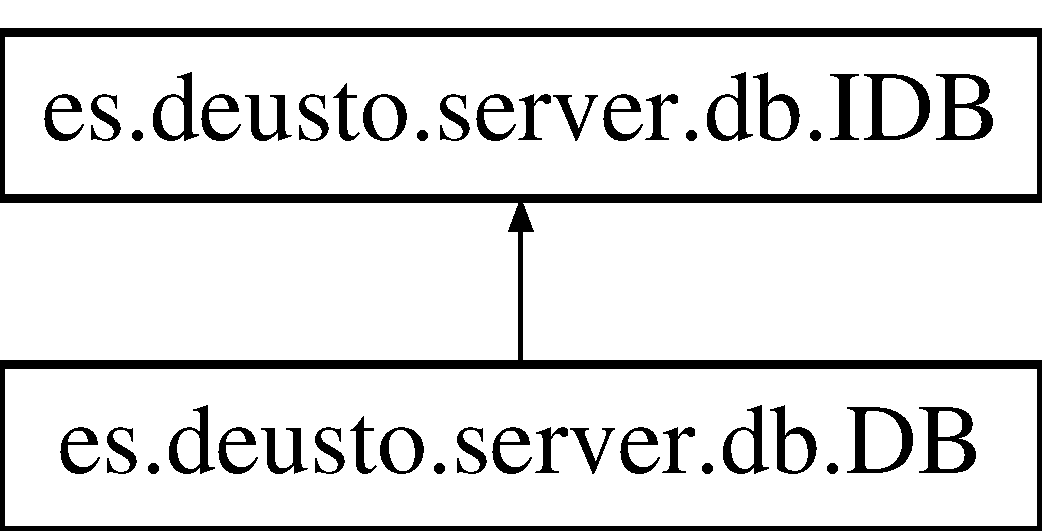
\includegraphics[height=2.000000cm]{interfacees_1_1deusto_1_1server_1_1db_1_1_i_d_b}
\end{center}
\end{figure}
\subsection*{Public Member Functions}
\begin{DoxyCompactItemize}
\item 
List$<$ \hyperlink{classes_1_1deusto_1_1server_1_1db_1_1data_1_1_product}{Product} $>$ \hyperlink{interfacees_1_1deusto_1_1server_1_1db_1_1_i_d_b_aba694290fde102c2eed31e505dd257fb}{get\+All\+Prod} ()
\item 
boolean \hyperlink{interfacees_1_1deusto_1_1server_1_1db_1_1_i_d_b_a64b43ced1334b833f7ee557badd2c5b7}{buy\+Prod} (String loginB, String loginS, String name, int amount)
\item 
boolean \hyperlink{interfacees_1_1deusto_1_1server_1_1db_1_1_i_d_b_a9d76b65686526214b48cd7d8f8dcdc86}{insert\+User} (\hyperlink{classes_1_1deusto_1_1server_1_1db_1_1data_1_1_user}{User} u)
\item 
boolean \hyperlink{interfacees_1_1deusto_1_1server_1_1db_1_1_i_d_b_a4c9c0a9511fde5b541a49de8f8399d28}{insert\+Prod} (\hyperlink{classes_1_1deusto_1_1server_1_1db_1_1data_1_1_product}{Product} p)
\item 
boolean \hyperlink{interfacees_1_1deusto_1_1server_1_1db_1_1_i_d_b_afcce296d82fa0a6fb8083215b3647663}{insert\+Money} (\hyperlink{classes_1_1deusto_1_1server_1_1db_1_1data_1_1_money}{Money} m)
\item 
\hyperlink{classes_1_1deusto_1_1server_1_1db_1_1data_1_1_product}{Product} \hyperlink{interfacees_1_1deusto_1_1server_1_1db_1_1_i_d_b_a8a4f72bb5148aff5b6f82679a7650b29}{show\+Prod} (String name)
\item 
\hyperlink{classes_1_1deusto_1_1server_1_1db_1_1data_1_1_user}{User} \hyperlink{interfacees_1_1deusto_1_1server_1_1db_1_1_i_d_b_aa2f6a5291fa8aa78d5a73b5878d17986}{show\+User} (String login)
\end{DoxyCompactItemize}


\subsection{Detailed Description}


Definition at line 8 of file I\+D\+B.\+java.



\subsection{Member Function Documentation}
\mbox{\Hypertarget{interfacees_1_1deusto_1_1server_1_1db_1_1_i_d_b_a64b43ced1334b833f7ee557badd2c5b7}\label{interfacees_1_1deusto_1_1server_1_1db_1_1_i_d_b_a64b43ced1334b833f7ee557badd2c5b7}} 
\index{es\+::deusto\+::server\+::db\+::\+I\+DB@{es\+::deusto\+::server\+::db\+::\+I\+DB}!buy\+Prod@{buy\+Prod}}
\index{buy\+Prod@{buy\+Prod}!es\+::deusto\+::server\+::db\+::\+I\+DB@{es\+::deusto\+::server\+::db\+::\+I\+DB}}
\subsubsection{\texorpdfstring{buy\+Prod()}{buyProd()}}
{\footnotesize\ttfamily boolean es.\+deusto.\+server.\+db.\+I\+D\+B.\+buy\+Prod (\begin{DoxyParamCaption}\item[{String}]{loginB,  }\item[{String}]{loginS,  }\item[{String}]{name,  }\item[{int}]{amount }\end{DoxyParamCaption})}



Implemented in \hyperlink{classes_1_1deusto_1_1server_1_1db_1_1_d_b_a06ce3aee905784e5ec88a8945452548e}{es.\+deusto.\+server.\+db.\+DB}.

\mbox{\Hypertarget{interfacees_1_1deusto_1_1server_1_1db_1_1_i_d_b_aba694290fde102c2eed31e505dd257fb}\label{interfacees_1_1deusto_1_1server_1_1db_1_1_i_d_b_aba694290fde102c2eed31e505dd257fb}} 
\index{es\+::deusto\+::server\+::db\+::\+I\+DB@{es\+::deusto\+::server\+::db\+::\+I\+DB}!get\+All\+Prod@{get\+All\+Prod}}
\index{get\+All\+Prod@{get\+All\+Prod}!es\+::deusto\+::server\+::db\+::\+I\+DB@{es\+::deusto\+::server\+::db\+::\+I\+DB}}
\subsubsection{\texorpdfstring{get\+All\+Prod()}{getAllProd()}}
{\footnotesize\ttfamily List$<$\hyperlink{classes_1_1deusto_1_1server_1_1db_1_1data_1_1_product}{Product}$>$ es.\+deusto.\+server.\+db.\+I\+D\+B.\+get\+All\+Prod (\begin{DoxyParamCaption}{ }\end{DoxyParamCaption})}



Implemented in \hyperlink{classes_1_1deusto_1_1server_1_1db_1_1_d_b_aa193a59efe6c2458d89fd751da935a3a}{es.\+deusto.\+server.\+db.\+DB}.

\mbox{\Hypertarget{interfacees_1_1deusto_1_1server_1_1db_1_1_i_d_b_afcce296d82fa0a6fb8083215b3647663}\label{interfacees_1_1deusto_1_1server_1_1db_1_1_i_d_b_afcce296d82fa0a6fb8083215b3647663}} 
\index{es\+::deusto\+::server\+::db\+::\+I\+DB@{es\+::deusto\+::server\+::db\+::\+I\+DB}!insert\+Money@{insert\+Money}}
\index{insert\+Money@{insert\+Money}!es\+::deusto\+::server\+::db\+::\+I\+DB@{es\+::deusto\+::server\+::db\+::\+I\+DB}}
\subsubsection{\texorpdfstring{insert\+Money()}{insertMoney()}}
{\footnotesize\ttfamily boolean es.\+deusto.\+server.\+db.\+I\+D\+B.\+insert\+Money (\begin{DoxyParamCaption}\item[{\hyperlink{classes_1_1deusto_1_1server_1_1db_1_1data_1_1_money}{Money}}]{m }\end{DoxyParamCaption})}



Implemented in \hyperlink{classes_1_1deusto_1_1server_1_1db_1_1_d_b_ab9a9acacfc8dadaeec7159c0886dfec2}{es.\+deusto.\+server.\+db.\+DB}.

\mbox{\Hypertarget{interfacees_1_1deusto_1_1server_1_1db_1_1_i_d_b_a4c9c0a9511fde5b541a49de8f8399d28}\label{interfacees_1_1deusto_1_1server_1_1db_1_1_i_d_b_a4c9c0a9511fde5b541a49de8f8399d28}} 
\index{es\+::deusto\+::server\+::db\+::\+I\+DB@{es\+::deusto\+::server\+::db\+::\+I\+DB}!insert\+Prod@{insert\+Prod}}
\index{insert\+Prod@{insert\+Prod}!es\+::deusto\+::server\+::db\+::\+I\+DB@{es\+::deusto\+::server\+::db\+::\+I\+DB}}
\subsubsection{\texorpdfstring{insert\+Prod()}{insertProd()}}
{\footnotesize\ttfamily boolean es.\+deusto.\+server.\+db.\+I\+D\+B.\+insert\+Prod (\begin{DoxyParamCaption}\item[{\hyperlink{classes_1_1deusto_1_1server_1_1db_1_1data_1_1_product}{Product}}]{p }\end{DoxyParamCaption})}



Implemented in \hyperlink{classes_1_1deusto_1_1server_1_1db_1_1_d_b_a2f5a50ff22834658b641ebf6bb7afbe6}{es.\+deusto.\+server.\+db.\+DB}.

\mbox{\Hypertarget{interfacees_1_1deusto_1_1server_1_1db_1_1_i_d_b_a9d76b65686526214b48cd7d8f8dcdc86}\label{interfacees_1_1deusto_1_1server_1_1db_1_1_i_d_b_a9d76b65686526214b48cd7d8f8dcdc86}} 
\index{es\+::deusto\+::server\+::db\+::\+I\+DB@{es\+::deusto\+::server\+::db\+::\+I\+DB}!insert\+User@{insert\+User}}
\index{insert\+User@{insert\+User}!es\+::deusto\+::server\+::db\+::\+I\+DB@{es\+::deusto\+::server\+::db\+::\+I\+DB}}
\subsubsection{\texorpdfstring{insert\+User()}{insertUser()}}
{\footnotesize\ttfamily boolean es.\+deusto.\+server.\+db.\+I\+D\+B.\+insert\+User (\begin{DoxyParamCaption}\item[{\hyperlink{classes_1_1deusto_1_1server_1_1db_1_1data_1_1_user}{User}}]{u }\end{DoxyParamCaption})}



Implemented in \hyperlink{classes_1_1deusto_1_1server_1_1db_1_1_d_b_a1070e289debd4f0fb5519c245c4e7ed7}{es.\+deusto.\+server.\+db.\+DB}.

\mbox{\Hypertarget{interfacees_1_1deusto_1_1server_1_1db_1_1_i_d_b_a8a4f72bb5148aff5b6f82679a7650b29}\label{interfacees_1_1deusto_1_1server_1_1db_1_1_i_d_b_a8a4f72bb5148aff5b6f82679a7650b29}} 
\index{es\+::deusto\+::server\+::db\+::\+I\+DB@{es\+::deusto\+::server\+::db\+::\+I\+DB}!show\+Prod@{show\+Prod}}
\index{show\+Prod@{show\+Prod}!es\+::deusto\+::server\+::db\+::\+I\+DB@{es\+::deusto\+::server\+::db\+::\+I\+DB}}
\subsubsection{\texorpdfstring{show\+Prod()}{showProd()}}
{\footnotesize\ttfamily \hyperlink{classes_1_1deusto_1_1server_1_1db_1_1data_1_1_product}{Product} es.\+deusto.\+server.\+db.\+I\+D\+B.\+show\+Prod (\begin{DoxyParamCaption}\item[{String}]{name }\end{DoxyParamCaption})}



Implemented in \hyperlink{classes_1_1deusto_1_1server_1_1db_1_1_d_b_a1c170a7c91ca5223560b4490738ccf56}{es.\+deusto.\+server.\+db.\+DB}.

\mbox{\Hypertarget{interfacees_1_1deusto_1_1server_1_1db_1_1_i_d_b_aa2f6a5291fa8aa78d5a73b5878d17986}\label{interfacees_1_1deusto_1_1server_1_1db_1_1_i_d_b_aa2f6a5291fa8aa78d5a73b5878d17986}} 
\index{es\+::deusto\+::server\+::db\+::\+I\+DB@{es\+::deusto\+::server\+::db\+::\+I\+DB}!show\+User@{show\+User}}
\index{show\+User@{show\+User}!es\+::deusto\+::server\+::db\+::\+I\+DB@{es\+::deusto\+::server\+::db\+::\+I\+DB}}
\subsubsection{\texorpdfstring{show\+User()}{showUser()}}
{\footnotesize\ttfamily \hyperlink{classes_1_1deusto_1_1server_1_1db_1_1data_1_1_user}{User} es.\+deusto.\+server.\+db.\+I\+D\+B.\+show\+User (\begin{DoxyParamCaption}\item[{String}]{login }\end{DoxyParamCaption})}



Implemented in \hyperlink{classes_1_1deusto_1_1server_1_1db_1_1_d_b_ac85523faea523033439a932bbcab2c7e}{es.\+deusto.\+server.\+db.\+DB}.



The documentation for this interface was generated from the following file\+:\begin{DoxyCompactItemize}
\item 
C\+:/\+Users/\+Oihane/git/\+S\+P\+Q03/spq03/src/main/java/es/deusto/server/db/\hyperlink{_i_d_b_8java}{I\+D\+B.\+java}\end{DoxyCompactItemize}

\hypertarget{interfacees_1_1deusto_1_1server_1_1remote_1_1_i_transferer}{}\section{es.\+deusto.\+server.\+remote.\+I\+Transferer Interface Reference}
\label{interfacees_1_1deusto_1_1server_1_1remote_1_1_i_transferer}\index{es.\+deusto.\+server.\+remote.\+I\+Transferer@{es.\+deusto.\+server.\+remote.\+I\+Transferer}}
Inheritance diagram for es.\+deusto.\+server.\+remote.\+I\+Transferer\+:\begin{figure}[H]
\begin{center}
\leavevmode
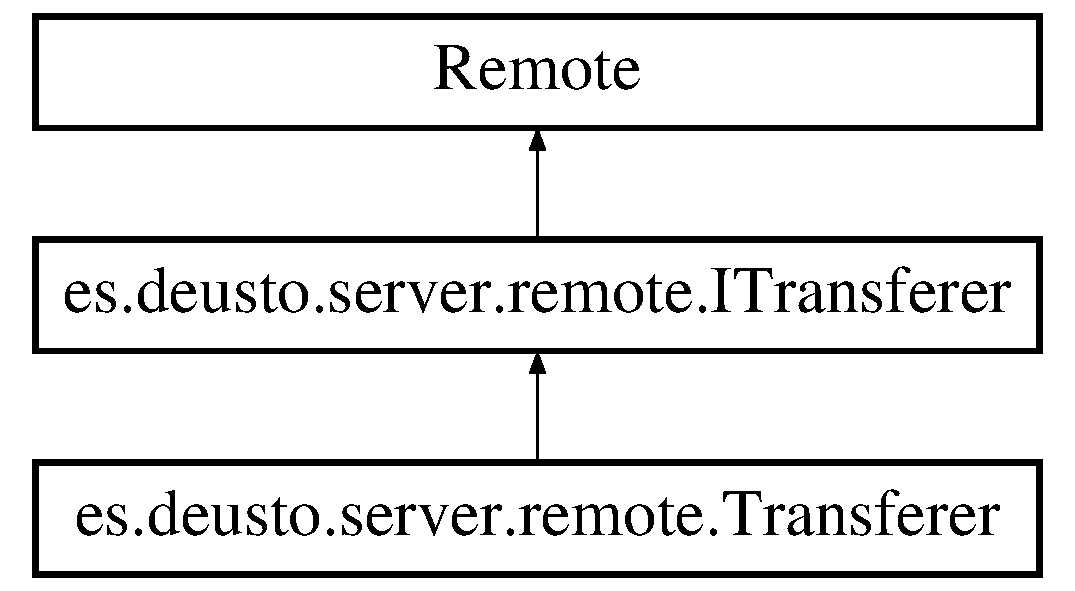
\includegraphics[height=3.000000cm]{interfacees_1_1deusto_1_1server_1_1remote_1_1_i_transferer}
\end{center}
\end{figure}
\subsection*{Public Member Functions}
\begin{DoxyCompactItemize}
\item 
boolean \hyperlink{interfacees_1_1deusto_1_1server_1_1remote_1_1_i_transferer_ab43399cfce0d84f6e27032a7c14865f6}{send\+Money} (String loginR, int amount, String loginS)  throws Remote\+Exception
\item 
Array\+List$<$ \hyperlink{classes_1_1deusto_1_1server_1_1db_1_1data_1_1_user}{User} $>$ \hyperlink{interfacees_1_1deusto_1_1server_1_1remote_1_1_i_transferer_aec6609427d773f075a78295a97888103}{get\+All\+User} ()  throws Remote\+Exception
\item 
boolean \hyperlink{interfacees_1_1deusto_1_1server_1_1remote_1_1_i_transferer_ab805207e578865de5bf2e69ca8942344}{register\+User} (\hyperlink{classes_1_1deusto_1_1server_1_1db_1_1data_1_1_user}{User} u)  throws Remote\+Exception
\item 
\hyperlink{classes_1_1deusto_1_1server_1_1db_1_1data_1_1_user}{User} \hyperlink{interfacees_1_1deusto_1_1server_1_1remote_1_1_i_transferer_ab767521556fc61bc5a39306080f00cae}{get\+User} (String login)  throws Remote\+Exception
\item 
Array\+List$<$ \hyperlink{classes_1_1deusto_1_1server_1_1db_1_1data_1_1_product}{Product} $>$ \hyperlink{interfacees_1_1deusto_1_1server_1_1remote_1_1_i_transferer_a71afa6799122b3f09805f86d2e58fc23}{get\+All\+Prod} ()  throws Remote\+Exception
\item 
\hyperlink{classes_1_1deusto_1_1server_1_1db_1_1data_1_1_product}{Product} \hyperlink{interfacees_1_1deusto_1_1server_1_1remote_1_1_i_transferer_a1fb33a5447e1647ffde8a01d180b8d99}{search\+Prod} (String name)  throws Remote\+Exception
\item 
boolean \hyperlink{interfacees_1_1deusto_1_1server_1_1remote_1_1_i_transferer_a86d92e8a78257551122807ae02259950}{buy\+Prod} (String loginB, \hyperlink{classes_1_1deusto_1_1server_1_1db_1_1data_1_1_product}{Product} p, int amount, String loginS)  throws Remote\+Exception
\item 
boolean \hyperlink{interfacees_1_1deusto_1_1server_1_1remote_1_1_i_transferer_a06629c7021aae4d2ce1a449726102ded}{register\+Prod} (\hyperlink{classes_1_1deusto_1_1server_1_1db_1_1data_1_1_product}{Product} p)  throws Remote\+Exception
\end{DoxyCompactItemize}


\subsection{Detailed Description}


Definition at line 10 of file I\+Transferer.\+java.



\subsection{Member Function Documentation}
\mbox{\Hypertarget{interfacees_1_1deusto_1_1server_1_1remote_1_1_i_transferer_a86d92e8a78257551122807ae02259950}\label{interfacees_1_1deusto_1_1server_1_1remote_1_1_i_transferer_a86d92e8a78257551122807ae02259950}} 
\index{es\+::deusto\+::server\+::remote\+::\+I\+Transferer@{es\+::deusto\+::server\+::remote\+::\+I\+Transferer}!buy\+Prod@{buy\+Prod}}
\index{buy\+Prod@{buy\+Prod}!es\+::deusto\+::server\+::remote\+::\+I\+Transferer@{es\+::deusto\+::server\+::remote\+::\+I\+Transferer}}
\subsubsection{\texorpdfstring{buy\+Prod()}{buyProd()}}
{\footnotesize\ttfamily boolean es.\+deusto.\+server.\+remote.\+I\+Transferer.\+buy\+Prod (\begin{DoxyParamCaption}\item[{String}]{loginB,  }\item[{\hyperlink{classes_1_1deusto_1_1server_1_1db_1_1data_1_1_product}{Product}}]{p,  }\item[{int}]{amount,  }\item[{String}]{loginS }\end{DoxyParamCaption}) throws Remote\+Exception}

This method allows the user with loginB to buy a product p to the user with loginS for the amount of money specified 
\begin{DoxyParams}{Parameters}
{\em loginB} & The PK that identifies the buyer \\
\hline
{\em p} & The Product to be bought \\
\hline
{\em amount} & The quantity to be spent on the transaction \\
\hline
{\em loginS} & The PK that identifies the seller \\
\hline
\end{DoxyParams}
\begin{DoxyReturn}{Returns}
Whether the product has been bought or not 
\end{DoxyReturn}

\begin{DoxyExceptions}{Exceptions}
{\em Remote\+Exception} & fails if there is a connection error \\
\hline
\end{DoxyExceptions}


Implemented in \hyperlink{classes_1_1deusto_1_1server_1_1remote_1_1_transferer_ad5868dd67ee9a53e7cdf0c30e08a3a1b}{es.\+deusto.\+server.\+remote.\+Transferer}.

\mbox{\Hypertarget{interfacees_1_1deusto_1_1server_1_1remote_1_1_i_transferer_a71afa6799122b3f09805f86d2e58fc23}\label{interfacees_1_1deusto_1_1server_1_1remote_1_1_i_transferer_a71afa6799122b3f09805f86d2e58fc23}} 
\index{es\+::deusto\+::server\+::remote\+::\+I\+Transferer@{es\+::deusto\+::server\+::remote\+::\+I\+Transferer}!get\+All\+Prod@{get\+All\+Prod}}
\index{get\+All\+Prod@{get\+All\+Prod}!es\+::deusto\+::server\+::remote\+::\+I\+Transferer@{es\+::deusto\+::server\+::remote\+::\+I\+Transferer}}
\subsubsection{\texorpdfstring{get\+All\+Prod()}{getAllProd()}}
{\footnotesize\ttfamily Array\+List$<$\hyperlink{classes_1_1deusto_1_1server_1_1db_1_1data_1_1_product}{Product}$>$ es.\+deusto.\+server.\+remote.\+I\+Transferer.\+get\+All\+Prod (\begin{DoxyParamCaption}{ }\end{DoxyParamCaption}) throws Remote\+Exception}

This method retrieves all the products inside the DB \begin{DoxyReturn}{Returns}
A list of all the products inside the DB 
\end{DoxyReturn}

\begin{DoxyExceptions}{Exceptions}
{\em Remote\+Exception} & fails if there is a connection error \\
\hline
\end{DoxyExceptions}


Implemented in \hyperlink{classes_1_1deusto_1_1server_1_1remote_1_1_transferer_a29cbb75edeb4e0973780fd379ef2b3fb}{es.\+deusto.\+server.\+remote.\+Transferer}.

\mbox{\Hypertarget{interfacees_1_1deusto_1_1server_1_1remote_1_1_i_transferer_aec6609427d773f075a78295a97888103}\label{interfacees_1_1deusto_1_1server_1_1remote_1_1_i_transferer_aec6609427d773f075a78295a97888103}} 
\index{es\+::deusto\+::server\+::remote\+::\+I\+Transferer@{es\+::deusto\+::server\+::remote\+::\+I\+Transferer}!get\+All\+User@{get\+All\+User}}
\index{get\+All\+User@{get\+All\+User}!es\+::deusto\+::server\+::remote\+::\+I\+Transferer@{es\+::deusto\+::server\+::remote\+::\+I\+Transferer}}
\subsubsection{\texorpdfstring{get\+All\+User()}{getAllUser()}}
{\footnotesize\ttfamily Array\+List$<$\hyperlink{classes_1_1deusto_1_1server_1_1db_1_1data_1_1_user}{User}$>$ es.\+deusto.\+server.\+remote.\+I\+Transferer.\+get\+All\+User (\begin{DoxyParamCaption}{ }\end{DoxyParamCaption}) throws Remote\+Exception}

This method returns the list of all users in the DB \begin{DoxyReturn}{Returns}
the list of users in the DB 
\end{DoxyReturn}

\begin{DoxyExceptions}{Exceptions}
{\em Remote\+Exception} & fails if there is a connection error \\
\hline
\end{DoxyExceptions}


Implemented in \hyperlink{classes_1_1deusto_1_1server_1_1remote_1_1_transferer_a613c0c3af149140e58488ce9d0745593}{es.\+deusto.\+server.\+remote.\+Transferer}.

\mbox{\Hypertarget{interfacees_1_1deusto_1_1server_1_1remote_1_1_i_transferer_ab767521556fc61bc5a39306080f00cae}\label{interfacees_1_1deusto_1_1server_1_1remote_1_1_i_transferer_ab767521556fc61bc5a39306080f00cae}} 
\index{es\+::deusto\+::server\+::remote\+::\+I\+Transferer@{es\+::deusto\+::server\+::remote\+::\+I\+Transferer}!get\+User@{get\+User}}
\index{get\+User@{get\+User}!es\+::deusto\+::server\+::remote\+::\+I\+Transferer@{es\+::deusto\+::server\+::remote\+::\+I\+Transferer}}
\subsubsection{\texorpdfstring{get\+User()}{getUser()}}
{\footnotesize\ttfamily \hyperlink{classes_1_1deusto_1_1server_1_1db_1_1data_1_1_user}{User} es.\+deusto.\+server.\+remote.\+I\+Transferer.\+get\+User (\begin{DoxyParamCaption}\item[{String}]{login }\end{DoxyParamCaption}) throws Remote\+Exception}

This method returns a user based on their username (login) 
\begin{DoxyParams}{Parameters}
{\em login} & The name of the user that wants to be retreived \\
\hline
\end{DoxyParams}
\begin{DoxyReturn}{Returns}
The user with the login name \char`\"{}login\char`\"{} 
\end{DoxyReturn}

\begin{DoxyExceptions}{Exceptions}
{\em Remote\+Exception} & fails if there is a connection error \\
\hline
\end{DoxyExceptions}


Implemented in \hyperlink{classes_1_1deusto_1_1server_1_1remote_1_1_transferer_a16976959aeb3080244422aeac061a23b}{es.\+deusto.\+server.\+remote.\+Transferer}.

\mbox{\Hypertarget{interfacees_1_1deusto_1_1server_1_1remote_1_1_i_transferer_a06629c7021aae4d2ce1a449726102ded}\label{interfacees_1_1deusto_1_1server_1_1remote_1_1_i_transferer_a06629c7021aae4d2ce1a449726102ded}} 
\index{es\+::deusto\+::server\+::remote\+::\+I\+Transferer@{es\+::deusto\+::server\+::remote\+::\+I\+Transferer}!register\+Prod@{register\+Prod}}
\index{register\+Prod@{register\+Prod}!es\+::deusto\+::server\+::remote\+::\+I\+Transferer@{es\+::deusto\+::server\+::remote\+::\+I\+Transferer}}
\subsubsection{\texorpdfstring{register\+Prod()}{registerProd()}}
{\footnotesize\ttfamily boolean es.\+deusto.\+server.\+remote.\+I\+Transferer.\+register\+Prod (\begin{DoxyParamCaption}\item[{\hyperlink{classes_1_1deusto_1_1server_1_1db_1_1data_1_1_product}{Product}}]{p }\end{DoxyParamCaption}) throws Remote\+Exception}

This method registers a product and returns if the transaction was done rightfully 
\begin{DoxyParams}{Parameters}
{\em p} & The product to register in the DB \\
\hline
\end{DoxyParams}
\begin{DoxyReturn}{Returns}
whether the product has been registered or not 
\end{DoxyReturn}

\begin{DoxyExceptions}{Exceptions}
{\em Remote\+Exception} & fails if there is a connection error \\
\hline
\end{DoxyExceptions}


Implemented in \hyperlink{classes_1_1deusto_1_1server_1_1remote_1_1_transferer_a64c1f3b57b74106df83335b124937afe}{es.\+deusto.\+server.\+remote.\+Transferer}.

\mbox{\Hypertarget{interfacees_1_1deusto_1_1server_1_1remote_1_1_i_transferer_ab805207e578865de5bf2e69ca8942344}\label{interfacees_1_1deusto_1_1server_1_1remote_1_1_i_transferer_ab805207e578865de5bf2e69ca8942344}} 
\index{es\+::deusto\+::server\+::remote\+::\+I\+Transferer@{es\+::deusto\+::server\+::remote\+::\+I\+Transferer}!register\+User@{register\+User}}
\index{register\+User@{register\+User}!es\+::deusto\+::server\+::remote\+::\+I\+Transferer@{es\+::deusto\+::server\+::remote\+::\+I\+Transferer}}
\subsubsection{\texorpdfstring{register\+User()}{registerUser()}}
{\footnotesize\ttfamily boolean es.\+deusto.\+server.\+remote.\+I\+Transferer.\+register\+User (\begin{DoxyParamCaption}\item[{\hyperlink{classes_1_1deusto_1_1server_1_1db_1_1data_1_1_user}{User}}]{u }\end{DoxyParamCaption}) throws Remote\+Exception}

This method registers a user and returns if the transaction was done rightfully 
\begin{DoxyParams}{Parameters}
{\em u} & The user to register in the DB \\
\hline
\end{DoxyParams}
\begin{DoxyReturn}{Returns}
whether the user has been registered or not 
\end{DoxyReturn}

\begin{DoxyExceptions}{Exceptions}
{\em Remote\+Exception} & fails if there is a connection error \\
\hline
\end{DoxyExceptions}


Implemented in \hyperlink{classes_1_1deusto_1_1server_1_1remote_1_1_transferer_a80e2dd7db595bdd8d39969e5d0e8ae7b}{es.\+deusto.\+server.\+remote.\+Transferer}.

\mbox{\Hypertarget{interfacees_1_1deusto_1_1server_1_1remote_1_1_i_transferer_a1fb33a5447e1647ffde8a01d180b8d99}\label{interfacees_1_1deusto_1_1server_1_1remote_1_1_i_transferer_a1fb33a5447e1647ffde8a01d180b8d99}} 
\index{es\+::deusto\+::server\+::remote\+::\+I\+Transferer@{es\+::deusto\+::server\+::remote\+::\+I\+Transferer}!search\+Prod@{search\+Prod}}
\index{search\+Prod@{search\+Prod}!es\+::deusto\+::server\+::remote\+::\+I\+Transferer@{es\+::deusto\+::server\+::remote\+::\+I\+Transferer}}
\subsubsection{\texorpdfstring{search\+Prod()}{searchProd()}}
{\footnotesize\ttfamily \hyperlink{classes_1_1deusto_1_1server_1_1db_1_1data_1_1_product}{Product} es.\+deusto.\+server.\+remote.\+I\+Transferer.\+search\+Prod (\begin{DoxyParamCaption}\item[{String}]{name }\end{DoxyParamCaption}) throws Remote\+Exception}

This method returns a Product based on its name 
\begin{DoxyParams}{Parameters}
{\em name} & The PK of the Product and the way to search it inside the DB \\
\hline
\end{DoxyParams}
\begin{DoxyReturn}{Returns}
An object Product that meets with the requirements 
\end{DoxyReturn}

\begin{DoxyExceptions}{Exceptions}
{\em Remote\+Exception} & fails if there is a connection error \\
\hline
\end{DoxyExceptions}


Implemented in \hyperlink{classes_1_1deusto_1_1server_1_1remote_1_1_transferer_ad6759f696eddd682b750f92ec41d1fcb}{es.\+deusto.\+server.\+remote.\+Transferer}.

\mbox{\Hypertarget{interfacees_1_1deusto_1_1server_1_1remote_1_1_i_transferer_ab43399cfce0d84f6e27032a7c14865f6}\label{interfacees_1_1deusto_1_1server_1_1remote_1_1_i_transferer_ab43399cfce0d84f6e27032a7c14865f6}} 
\index{es\+::deusto\+::server\+::remote\+::\+I\+Transferer@{es\+::deusto\+::server\+::remote\+::\+I\+Transferer}!send\+Money@{send\+Money}}
\index{send\+Money@{send\+Money}!es\+::deusto\+::server\+::remote\+::\+I\+Transferer@{es\+::deusto\+::server\+::remote\+::\+I\+Transferer}}
\subsubsection{\texorpdfstring{send\+Money()}{sendMoney()}}
{\footnotesize\ttfamily boolean es.\+deusto.\+server.\+remote.\+I\+Transferer.\+send\+Money (\begin{DoxyParamCaption}\item[{String}]{loginR,  }\item[{int}]{amount,  }\item[{String}]{loginS }\end{DoxyParamCaption}) throws Remote\+Exception}

This method allows the user with loginS to send an amount to the user with loginR 
\begin{DoxyParams}{Parameters}
{\em loginR} & the name of the user that receives the money \\
\hline
{\em amount} & the number of money sent \\
\hline
{\em loginS} & the name of the user that sends the money \\
\hline
\end{DoxyParams}
\begin{DoxyReturn}{Returns}
whether the money has been sent or not 
\end{DoxyReturn}

\begin{DoxyExceptions}{Exceptions}
{\em Remote\+Exception} & fails if there is a connection error \\
\hline
\end{DoxyExceptions}


Implemented in \hyperlink{classes_1_1deusto_1_1server_1_1remote_1_1_transferer_ad1eb84155ba0c457645f2ad53725320d}{es.\+deusto.\+server.\+remote.\+Transferer}.



The documentation for this interface was generated from the following file\+:\begin{DoxyCompactItemize}
\item 
C\+:/\+Users/\+Oihane/git/\+S\+P\+Q03/spq03/src/main/java/es/deusto/server/remote/\hyperlink{_i_transferer_8java}{I\+Transferer.\+java}\end{DoxyCompactItemize}

\hypertarget{classes_1_1deusto_1_1server_1_1_j_unit_test}{}\section{es.\+deusto.\+server.\+J\+Unit\+Test Class Reference}
\label{classes_1_1deusto_1_1server_1_1_j_unit_test}\index{es.\+deusto.\+server.\+J\+Unit\+Test@{es.\+deusto.\+server.\+J\+Unit\+Test}}
\subsection*{Public Member Functions}
\begin{DoxyCompactItemize}
\item 
void \hyperlink{classes_1_1deusto_1_1server_1_1_j_unit_test_a70ed61bac7b0101aed52c1ea8d2a58cf}{set\+Up\+User} ()
\item 
void \hyperlink{classes_1_1deusto_1_1server_1_1_j_unit_test_a2bdde69e0f41e4977c4ad76fa2cd0b95}{stablish\+Connection} ()
\item 
void \hyperlink{classes_1_1deusto_1_1server_1_1_j_unit_test_a11102e5000a6ff4c211c7243ab938117}{Register\+Product\+Test} ()
\item 
void \hyperlink{classes_1_1deusto_1_1server_1_1_j_unit_test_a0b87ea354f96ee4432cb5b5efd1604c5}{test\+Register\+User} ()
\item 
void \hyperlink{classes_1_1deusto_1_1server_1_1_j_unit_test_a534cdf24e98dd7d1d6a965e2f5ab75be}{test\+Get\+User} ()
\item 
void \hyperlink{classes_1_1deusto_1_1server_1_1_j_unit_test_a1a63f85e03a2c22d000ae9f3d2697159}{test\+Search\+Product} ()
\item 
void \hyperlink{classes_1_1deusto_1_1server_1_1_j_unit_test_a642a3012a65a9d81b891321efba4e2d3}{test\+Store\+User} ()
\item 
void \hyperlink{classes_1_1deusto_1_1server_1_1_j_unit_test_adce751e460d92b4bf6f82f246f552ab8}{test\+Retrieve\+User} ()
\item 
void \hyperlink{classes_1_1deusto_1_1server_1_1_j_unit_test_a47ec4408530333c9577359f7be9d78fa}{test\+Store\+Product} ()
\item 
void \hyperlink{classes_1_1deusto_1_1server_1_1_j_unit_test_a9a74c617f8cd970204919217df16090d}{test\+Get\+All\+Prod} ()
\item 
void \hyperlink{classes_1_1deusto_1_1server_1_1_j_unit_test_a6af88e3e3ad84aed02c23286c5d2a178}{test\+Update\+Product} ()
\item 
void \hyperlink{classes_1_1deusto_1_1server_1_1_j_unit_test_aeb535acfcc2efe9f6402d1d6c515d2d8}{test\+Buy\+Product} ()
\item 
void \hyperlink{classes_1_1deusto_1_1server_1_1_j_unit_test_aaad8cae59ca19f9dba654a12f695dbd0}{test\+Update\+Money} ()
\item 
void \hyperlink{classes_1_1deusto_1_1server_1_1_j_unit_test_a6863eca45b97fd4cce293b9ee705da6f}{test\+Store\+Money} ()
\item 
void \hyperlink{classes_1_1deusto_1_1server_1_1_j_unit_test_acd22c583e2d8276c76df148ddca3d716}{test\+Retrieve\+Money} ()
\item 
void \hyperlink{classes_1_1deusto_1_1server_1_1_j_unit_test_a3d96e27fee6cffb14a0f43b9516c9eb9}{test\+Send\+Money} ()
\item 
void \hyperlink{classes_1_1deusto_1_1server_1_1_j_unit_test_a7f488e3ee6b4751aaffd8ac74edc828d}{test\+Get\+Sender} ()
\item 
void \hyperlink{classes_1_1deusto_1_1server_1_1_j_unit_test_a545a0934031db41d9333d9106c050ae4}{test\+Get\+Prod} ()
\item 
void \hyperlink{classes_1_1deusto_1_1server_1_1_j_unit_test_aad5e9f503b6938b10c7935af68ae99fa}{test\+Get\+Amount} ()
\item 
void \hyperlink{classes_1_1deusto_1_1server_1_1_j_unit_test_a9e4938a911e40d6f36531639482d09a8}{test\+Get\+Name} ()
\item 
void \hyperlink{classes_1_1deusto_1_1server_1_1_j_unit_test_adfe6c8de32fe489f31f62338a475729e}{test\+Get\+Characteristics} ()
\item 
void \hyperlink{classes_1_1deusto_1_1server_1_1_j_unit_test_a6c7354d3207f6f6e8778d1b85fd31746}{test\+Get\+Login} ()
\item 
void \hyperlink{classes_1_1deusto_1_1server_1_1_j_unit_test_aac72817037da417d5eb5b32078971398}{test\+Get\+Password} ()
\item 
void \hyperlink{classes_1_1deusto_1_1server_1_1_j_unit_test_a6204483b84dccff7e6dd2e98d9b20b1b}{test\+Get\+Money} ()
\end{DoxyCompactItemize}
\subsection*{Static Public Member Functions}
\begin{DoxyCompactItemize}
\item 
static junit.\+framework.\+Test \hyperlink{classes_1_1deusto_1_1server_1_1_j_unit_test_ae981ce8acebd33a65ebe3160ceeac17b}{suite} ()
\item 
static void \hyperlink{classes_1_1deusto_1_1server_1_1_j_unit_test_af386e60b196afb70391c05e71563efd6}{set\+Up} ()
\item 
static void \hyperlink{classes_1_1deusto_1_1server_1_1_j_unit_test_a6773c13994c33488b0f6ca363c92417a}{tear\+Down} ()
\end{DoxyCompactItemize}


\subsection{Detailed Description}


Definition at line 44 of file J\+Unit\+Test.\+java.



\subsection{Member Function Documentation}
\mbox{\Hypertarget{classes_1_1deusto_1_1server_1_1_j_unit_test_a11102e5000a6ff4c211c7243ab938117}\label{classes_1_1deusto_1_1server_1_1_j_unit_test_a11102e5000a6ff4c211c7243ab938117}} 
\index{es\+::deusto\+::server\+::\+J\+Unit\+Test@{es\+::deusto\+::server\+::\+J\+Unit\+Test}!Register\+Product\+Test@{Register\+Product\+Test}}
\index{Register\+Product\+Test@{Register\+Product\+Test}!es\+::deusto\+::server\+::\+J\+Unit\+Test@{es\+::deusto\+::server\+::\+J\+Unit\+Test}}
\subsubsection{\texorpdfstring{Register\+Product\+Test()}{RegisterProductTest()}}
{\footnotesize\ttfamily void es.\+deusto.\+server.\+J\+Unit\+Test.\+Register\+Product\+Test (\begin{DoxyParamCaption}{ }\end{DoxyParamCaption})}



Definition at line 223 of file J\+Unit\+Test.\+java.

\mbox{\Hypertarget{classes_1_1deusto_1_1server_1_1_j_unit_test_af386e60b196afb70391c05e71563efd6}\label{classes_1_1deusto_1_1server_1_1_j_unit_test_af386e60b196afb70391c05e71563efd6}} 
\index{es\+::deusto\+::server\+::\+J\+Unit\+Test@{es\+::deusto\+::server\+::\+J\+Unit\+Test}!set\+Up@{set\+Up}}
\index{set\+Up@{set\+Up}!es\+::deusto\+::server\+::\+J\+Unit\+Test@{es\+::deusto\+::server\+::\+J\+Unit\+Test}}
\subsubsection{\texorpdfstring{set\+Up()}{setUp()}}
{\footnotesize\ttfamily static void es.\+deusto.\+server.\+J\+Unit\+Test.\+set\+Up (\begin{DoxyParamCaption}{ }\end{DoxyParamCaption})\hspace{0.3cm}{\ttfamily [static]}}



Definition at line 67 of file J\+Unit\+Test.\+java.

\mbox{\Hypertarget{classes_1_1deusto_1_1server_1_1_j_unit_test_a70ed61bac7b0101aed52c1ea8d2a58cf}\label{classes_1_1deusto_1_1server_1_1_j_unit_test_a70ed61bac7b0101aed52c1ea8d2a58cf}} 
\index{es\+::deusto\+::server\+::\+J\+Unit\+Test@{es\+::deusto\+::server\+::\+J\+Unit\+Test}!set\+Up\+User@{set\+Up\+User}}
\index{set\+Up\+User@{set\+Up\+User}!es\+::deusto\+::server\+::\+J\+Unit\+Test@{es\+::deusto\+::server\+::\+J\+Unit\+Test}}
\subsubsection{\texorpdfstring{set\+Up\+User()}{setUpUser()}}
{\footnotesize\ttfamily void es.\+deusto.\+server.\+J\+Unit\+Test.\+set\+Up\+User (\begin{DoxyParamCaption}{ }\end{DoxyParamCaption})}



Definition at line 157 of file J\+Unit\+Test.\+java.

\mbox{\Hypertarget{classes_1_1deusto_1_1server_1_1_j_unit_test_a2bdde69e0f41e4977c4ad76fa2cd0b95}\label{classes_1_1deusto_1_1server_1_1_j_unit_test_a2bdde69e0f41e4977c4ad76fa2cd0b95}} 
\index{es\+::deusto\+::server\+::\+J\+Unit\+Test@{es\+::deusto\+::server\+::\+J\+Unit\+Test}!stablish\+Connection@{stablish\+Connection}}
\index{stablish\+Connection@{stablish\+Connection}!es\+::deusto\+::server\+::\+J\+Unit\+Test@{es\+::deusto\+::server\+::\+J\+Unit\+Test}}
\subsubsection{\texorpdfstring{stablish\+Connection()}{stablishConnection()}}
{\footnotesize\ttfamily void es.\+deusto.\+server.\+J\+Unit\+Test.\+stablish\+Connection (\begin{DoxyParamCaption}{ }\end{DoxyParamCaption})}



Definition at line 210 of file J\+Unit\+Test.\+java.

\mbox{\Hypertarget{classes_1_1deusto_1_1server_1_1_j_unit_test_ae981ce8acebd33a65ebe3160ceeac17b}\label{classes_1_1deusto_1_1server_1_1_j_unit_test_ae981ce8acebd33a65ebe3160ceeac17b}} 
\index{es\+::deusto\+::server\+::\+J\+Unit\+Test@{es\+::deusto\+::server\+::\+J\+Unit\+Test}!suite@{suite}}
\index{suite@{suite}!es\+::deusto\+::server\+::\+J\+Unit\+Test@{es\+::deusto\+::server\+::\+J\+Unit\+Test}}
\subsubsection{\texorpdfstring{suite()}{suite()}}
{\footnotesize\ttfamily static junit.\+framework.\+Test es.\+deusto.\+server.\+J\+Unit\+Test.\+suite (\begin{DoxyParamCaption}{ }\end{DoxyParamCaption})\hspace{0.3cm}{\ttfamily [static]}}



Definition at line 62 of file J\+Unit\+Test.\+java.

\mbox{\Hypertarget{classes_1_1deusto_1_1server_1_1_j_unit_test_a6773c13994c33488b0f6ca363c92417a}\label{classes_1_1deusto_1_1server_1_1_j_unit_test_a6773c13994c33488b0f6ca363c92417a}} 
\index{es\+::deusto\+::server\+::\+J\+Unit\+Test@{es\+::deusto\+::server\+::\+J\+Unit\+Test}!tear\+Down@{tear\+Down}}
\index{tear\+Down@{tear\+Down}!es\+::deusto\+::server\+::\+J\+Unit\+Test@{es\+::deusto\+::server\+::\+J\+Unit\+Test}}
\subsubsection{\texorpdfstring{tear\+Down()}{tearDown()}}
{\footnotesize\ttfamily static void es.\+deusto.\+server.\+J\+Unit\+Test.\+tear\+Down (\begin{DoxyParamCaption}{ }\end{DoxyParamCaption})\hspace{0.3cm}{\ttfamily [static]}}



Definition at line 442 of file J\+Unit\+Test.\+java.

\mbox{\Hypertarget{classes_1_1deusto_1_1server_1_1_j_unit_test_aeb535acfcc2efe9f6402d1d6c515d2d8}\label{classes_1_1deusto_1_1server_1_1_j_unit_test_aeb535acfcc2efe9f6402d1d6c515d2d8}} 
\index{es\+::deusto\+::server\+::\+J\+Unit\+Test@{es\+::deusto\+::server\+::\+J\+Unit\+Test}!test\+Buy\+Product@{test\+Buy\+Product}}
\index{test\+Buy\+Product@{test\+Buy\+Product}!es\+::deusto\+::server\+::\+J\+Unit\+Test@{es\+::deusto\+::server\+::\+J\+Unit\+Test}}
\subsubsection{\texorpdfstring{test\+Buy\+Product()}{testBuyProduct()}}
{\footnotesize\ttfamily void es.\+deusto.\+server.\+J\+Unit\+Test.\+test\+Buy\+Product (\begin{DoxyParamCaption}{ }\end{DoxyParamCaption})}



Definition at line 357 of file J\+Unit\+Test.\+java.

\mbox{\Hypertarget{classes_1_1deusto_1_1server_1_1_j_unit_test_a9a74c617f8cd970204919217df16090d}\label{classes_1_1deusto_1_1server_1_1_j_unit_test_a9a74c617f8cd970204919217df16090d}} 
\index{es\+::deusto\+::server\+::\+J\+Unit\+Test@{es\+::deusto\+::server\+::\+J\+Unit\+Test}!test\+Get\+All\+Prod@{test\+Get\+All\+Prod}}
\index{test\+Get\+All\+Prod@{test\+Get\+All\+Prod}!es\+::deusto\+::server\+::\+J\+Unit\+Test@{es\+::deusto\+::server\+::\+J\+Unit\+Test}}
\subsubsection{\texorpdfstring{test\+Get\+All\+Prod()}{testGetAllProd()}}
{\footnotesize\ttfamily void es.\+deusto.\+server.\+J\+Unit\+Test.\+test\+Get\+All\+Prod (\begin{DoxyParamCaption}{ }\end{DoxyParamCaption})}



Definition at line 331 of file J\+Unit\+Test.\+java.

\mbox{\Hypertarget{classes_1_1deusto_1_1server_1_1_j_unit_test_aad5e9f503b6938b10c7935af68ae99fa}\label{classes_1_1deusto_1_1server_1_1_j_unit_test_aad5e9f503b6938b10c7935af68ae99fa}} 
\index{es\+::deusto\+::server\+::\+J\+Unit\+Test@{es\+::deusto\+::server\+::\+J\+Unit\+Test}!test\+Get\+Amount@{test\+Get\+Amount}}
\index{test\+Get\+Amount@{test\+Get\+Amount}!es\+::deusto\+::server\+::\+J\+Unit\+Test@{es\+::deusto\+::server\+::\+J\+Unit\+Test}}
\subsubsection{\texorpdfstring{test\+Get\+Amount()}{testGetAmount()}}
{\footnotesize\ttfamily void es.\+deusto.\+server.\+J\+Unit\+Test.\+test\+Get\+Amount (\begin{DoxyParamCaption}{ }\end{DoxyParamCaption})}



Definition at line 405 of file J\+Unit\+Test.\+java.

\mbox{\Hypertarget{classes_1_1deusto_1_1server_1_1_j_unit_test_adfe6c8de32fe489f31f62338a475729e}\label{classes_1_1deusto_1_1server_1_1_j_unit_test_adfe6c8de32fe489f31f62338a475729e}} 
\index{es\+::deusto\+::server\+::\+J\+Unit\+Test@{es\+::deusto\+::server\+::\+J\+Unit\+Test}!test\+Get\+Characteristics@{test\+Get\+Characteristics}}
\index{test\+Get\+Characteristics@{test\+Get\+Characteristics}!es\+::deusto\+::server\+::\+J\+Unit\+Test@{es\+::deusto\+::server\+::\+J\+Unit\+Test}}
\subsubsection{\texorpdfstring{test\+Get\+Characteristics()}{testGetCharacteristics()}}
{\footnotesize\ttfamily void es.\+deusto.\+server.\+J\+Unit\+Test.\+test\+Get\+Characteristics (\begin{DoxyParamCaption}{ }\end{DoxyParamCaption})}



Definition at line 417 of file J\+Unit\+Test.\+java.

\mbox{\Hypertarget{classes_1_1deusto_1_1server_1_1_j_unit_test_a6c7354d3207f6f6e8778d1b85fd31746}\label{classes_1_1deusto_1_1server_1_1_j_unit_test_a6c7354d3207f6f6e8778d1b85fd31746}} 
\index{es\+::deusto\+::server\+::\+J\+Unit\+Test@{es\+::deusto\+::server\+::\+J\+Unit\+Test}!test\+Get\+Login@{test\+Get\+Login}}
\index{test\+Get\+Login@{test\+Get\+Login}!es\+::deusto\+::server\+::\+J\+Unit\+Test@{es\+::deusto\+::server\+::\+J\+Unit\+Test}}
\subsubsection{\texorpdfstring{test\+Get\+Login()}{testGetLogin()}}
{\footnotesize\ttfamily void es.\+deusto.\+server.\+J\+Unit\+Test.\+test\+Get\+Login (\begin{DoxyParamCaption}{ }\end{DoxyParamCaption})}



Definition at line 423 of file J\+Unit\+Test.\+java.

\mbox{\Hypertarget{classes_1_1deusto_1_1server_1_1_j_unit_test_a6204483b84dccff7e6dd2e98d9b20b1b}\label{classes_1_1deusto_1_1server_1_1_j_unit_test_a6204483b84dccff7e6dd2e98d9b20b1b}} 
\index{es\+::deusto\+::server\+::\+J\+Unit\+Test@{es\+::deusto\+::server\+::\+J\+Unit\+Test}!test\+Get\+Money@{test\+Get\+Money}}
\index{test\+Get\+Money@{test\+Get\+Money}!es\+::deusto\+::server\+::\+J\+Unit\+Test@{es\+::deusto\+::server\+::\+J\+Unit\+Test}}
\subsubsection{\texorpdfstring{test\+Get\+Money()}{testGetMoney()}}
{\footnotesize\ttfamily void es.\+deusto.\+server.\+J\+Unit\+Test.\+test\+Get\+Money (\begin{DoxyParamCaption}{ }\end{DoxyParamCaption})}



Definition at line 436 of file J\+Unit\+Test.\+java.

\mbox{\Hypertarget{classes_1_1deusto_1_1server_1_1_j_unit_test_a9e4938a911e40d6f36531639482d09a8}\label{classes_1_1deusto_1_1server_1_1_j_unit_test_a9e4938a911e40d6f36531639482d09a8}} 
\index{es\+::deusto\+::server\+::\+J\+Unit\+Test@{es\+::deusto\+::server\+::\+J\+Unit\+Test}!test\+Get\+Name@{test\+Get\+Name}}
\index{test\+Get\+Name@{test\+Get\+Name}!es\+::deusto\+::server\+::\+J\+Unit\+Test@{es\+::deusto\+::server\+::\+J\+Unit\+Test}}
\subsubsection{\texorpdfstring{test\+Get\+Name()}{testGetName()}}
{\footnotesize\ttfamily void es.\+deusto.\+server.\+J\+Unit\+Test.\+test\+Get\+Name (\begin{DoxyParamCaption}{ }\end{DoxyParamCaption})}



Definition at line 411 of file J\+Unit\+Test.\+java.

\mbox{\Hypertarget{classes_1_1deusto_1_1server_1_1_j_unit_test_aac72817037da417d5eb5b32078971398}\label{classes_1_1deusto_1_1server_1_1_j_unit_test_aac72817037da417d5eb5b32078971398}} 
\index{es\+::deusto\+::server\+::\+J\+Unit\+Test@{es\+::deusto\+::server\+::\+J\+Unit\+Test}!test\+Get\+Password@{test\+Get\+Password}}
\index{test\+Get\+Password@{test\+Get\+Password}!es\+::deusto\+::server\+::\+J\+Unit\+Test@{es\+::deusto\+::server\+::\+J\+Unit\+Test}}
\subsubsection{\texorpdfstring{test\+Get\+Password()}{testGetPassword()}}
{\footnotesize\ttfamily void es.\+deusto.\+server.\+J\+Unit\+Test.\+test\+Get\+Password (\begin{DoxyParamCaption}{ }\end{DoxyParamCaption})}



Definition at line 430 of file J\+Unit\+Test.\+java.

\mbox{\Hypertarget{classes_1_1deusto_1_1server_1_1_j_unit_test_a545a0934031db41d9333d9106c050ae4}\label{classes_1_1deusto_1_1server_1_1_j_unit_test_a545a0934031db41d9333d9106c050ae4}} 
\index{es\+::deusto\+::server\+::\+J\+Unit\+Test@{es\+::deusto\+::server\+::\+J\+Unit\+Test}!test\+Get\+Prod@{test\+Get\+Prod}}
\index{test\+Get\+Prod@{test\+Get\+Prod}!es\+::deusto\+::server\+::\+J\+Unit\+Test@{es\+::deusto\+::server\+::\+J\+Unit\+Test}}
\subsubsection{\texorpdfstring{test\+Get\+Prod()}{testGetProd()}}
{\footnotesize\ttfamily void es.\+deusto.\+server.\+J\+Unit\+Test.\+test\+Get\+Prod (\begin{DoxyParamCaption}{ }\end{DoxyParamCaption})}



Definition at line 398 of file J\+Unit\+Test.\+java.

\mbox{\Hypertarget{classes_1_1deusto_1_1server_1_1_j_unit_test_a7f488e3ee6b4751aaffd8ac74edc828d}\label{classes_1_1deusto_1_1server_1_1_j_unit_test_a7f488e3ee6b4751aaffd8ac74edc828d}} 
\index{es\+::deusto\+::server\+::\+J\+Unit\+Test@{es\+::deusto\+::server\+::\+J\+Unit\+Test}!test\+Get\+Sender@{test\+Get\+Sender}}
\index{test\+Get\+Sender@{test\+Get\+Sender}!es\+::deusto\+::server\+::\+J\+Unit\+Test@{es\+::deusto\+::server\+::\+J\+Unit\+Test}}
\subsubsection{\texorpdfstring{test\+Get\+Sender()}{testGetSender()}}
{\footnotesize\ttfamily void es.\+deusto.\+server.\+J\+Unit\+Test.\+test\+Get\+Sender (\begin{DoxyParamCaption}{ }\end{DoxyParamCaption})}



Definition at line 390 of file J\+Unit\+Test.\+java.

\mbox{\Hypertarget{classes_1_1deusto_1_1server_1_1_j_unit_test_a534cdf24e98dd7d1d6a965e2f5ab75be}\label{classes_1_1deusto_1_1server_1_1_j_unit_test_a534cdf24e98dd7d1d6a965e2f5ab75be}} 
\index{es\+::deusto\+::server\+::\+J\+Unit\+Test@{es\+::deusto\+::server\+::\+J\+Unit\+Test}!test\+Get\+User@{test\+Get\+User}}
\index{test\+Get\+User@{test\+Get\+User}!es\+::deusto\+::server\+::\+J\+Unit\+Test@{es\+::deusto\+::server\+::\+J\+Unit\+Test}}
\subsubsection{\texorpdfstring{test\+Get\+User()}{testGetUser()}}
{\footnotesize\ttfamily void es.\+deusto.\+server.\+J\+Unit\+Test.\+test\+Get\+User (\begin{DoxyParamCaption}{ }\end{DoxyParamCaption})}



Definition at line 243 of file J\+Unit\+Test.\+java.

\mbox{\Hypertarget{classes_1_1deusto_1_1server_1_1_j_unit_test_a0b87ea354f96ee4432cb5b5efd1604c5}\label{classes_1_1deusto_1_1server_1_1_j_unit_test_a0b87ea354f96ee4432cb5b5efd1604c5}} 
\index{es\+::deusto\+::server\+::\+J\+Unit\+Test@{es\+::deusto\+::server\+::\+J\+Unit\+Test}!test\+Register\+User@{test\+Register\+User}}
\index{test\+Register\+User@{test\+Register\+User}!es\+::deusto\+::server\+::\+J\+Unit\+Test@{es\+::deusto\+::server\+::\+J\+Unit\+Test}}
\subsubsection{\texorpdfstring{test\+Register\+User()}{testRegisterUser()}}
{\footnotesize\ttfamily void es.\+deusto.\+server.\+J\+Unit\+Test.\+test\+Register\+User (\begin{DoxyParamCaption}{ }\end{DoxyParamCaption})}



Definition at line 234 of file J\+Unit\+Test.\+java.

\mbox{\Hypertarget{classes_1_1deusto_1_1server_1_1_j_unit_test_acd22c583e2d8276c76df148ddca3d716}\label{classes_1_1deusto_1_1server_1_1_j_unit_test_acd22c583e2d8276c76df148ddca3d716}} 
\index{es\+::deusto\+::server\+::\+J\+Unit\+Test@{es\+::deusto\+::server\+::\+J\+Unit\+Test}!test\+Retrieve\+Money@{test\+Retrieve\+Money}}
\index{test\+Retrieve\+Money@{test\+Retrieve\+Money}!es\+::deusto\+::server\+::\+J\+Unit\+Test@{es\+::deusto\+::server\+::\+J\+Unit\+Test}}
\subsubsection{\texorpdfstring{test\+Retrieve\+Money()}{testRetrieveMoney()}}
{\footnotesize\ttfamily void es.\+deusto.\+server.\+J\+Unit\+Test.\+test\+Retrieve\+Money (\begin{DoxyParamCaption}{ }\end{DoxyParamCaption})}



Definition at line 380 of file J\+Unit\+Test.\+java.

\mbox{\Hypertarget{classes_1_1deusto_1_1server_1_1_j_unit_test_adce751e460d92b4bf6f82f246f552ab8}\label{classes_1_1deusto_1_1server_1_1_j_unit_test_adce751e460d92b4bf6f82f246f552ab8}} 
\index{es\+::deusto\+::server\+::\+J\+Unit\+Test@{es\+::deusto\+::server\+::\+J\+Unit\+Test}!test\+Retrieve\+User@{test\+Retrieve\+User}}
\index{test\+Retrieve\+User@{test\+Retrieve\+User}!es\+::deusto\+::server\+::\+J\+Unit\+Test@{es\+::deusto\+::server\+::\+J\+Unit\+Test}}
\subsubsection{\texorpdfstring{test\+Retrieve\+User()}{testRetrieveUser()}}
{\footnotesize\ttfamily void es.\+deusto.\+server.\+J\+Unit\+Test.\+test\+Retrieve\+User (\begin{DoxyParamCaption}{ }\end{DoxyParamCaption})}



Definition at line 287 of file J\+Unit\+Test.\+java.

\mbox{\Hypertarget{classes_1_1deusto_1_1server_1_1_j_unit_test_a1a63f85e03a2c22d000ae9f3d2697159}\label{classes_1_1deusto_1_1server_1_1_j_unit_test_a1a63f85e03a2c22d000ae9f3d2697159}} 
\index{es\+::deusto\+::server\+::\+J\+Unit\+Test@{es\+::deusto\+::server\+::\+J\+Unit\+Test}!test\+Search\+Product@{test\+Search\+Product}}
\index{test\+Search\+Product@{test\+Search\+Product}!es\+::deusto\+::server\+::\+J\+Unit\+Test@{es\+::deusto\+::server\+::\+J\+Unit\+Test}}
\subsubsection{\texorpdfstring{test\+Search\+Product()}{testSearchProduct()}}
{\footnotesize\ttfamily void es.\+deusto.\+server.\+J\+Unit\+Test.\+test\+Search\+Product (\begin{DoxyParamCaption}{ }\end{DoxyParamCaption})}



Definition at line 255 of file J\+Unit\+Test.\+java.

\mbox{\Hypertarget{classes_1_1deusto_1_1server_1_1_j_unit_test_a3d96e27fee6cffb14a0f43b9516c9eb9}\label{classes_1_1deusto_1_1server_1_1_j_unit_test_a3d96e27fee6cffb14a0f43b9516c9eb9}} 
\index{es\+::deusto\+::server\+::\+J\+Unit\+Test@{es\+::deusto\+::server\+::\+J\+Unit\+Test}!test\+Send\+Money@{test\+Send\+Money}}
\index{test\+Send\+Money@{test\+Send\+Money}!es\+::deusto\+::server\+::\+J\+Unit\+Test@{es\+::deusto\+::server\+::\+J\+Unit\+Test}}
\subsubsection{\texorpdfstring{test\+Send\+Money()}{testSendMoney()}}
{\footnotesize\ttfamily void es.\+deusto.\+server.\+J\+Unit\+Test.\+test\+Send\+Money (\begin{DoxyParamCaption}{ }\end{DoxyParamCaption})}



Definition at line 385 of file J\+Unit\+Test.\+java.

\mbox{\Hypertarget{classes_1_1deusto_1_1server_1_1_j_unit_test_a6863eca45b97fd4cce293b9ee705da6f}\label{classes_1_1deusto_1_1server_1_1_j_unit_test_a6863eca45b97fd4cce293b9ee705da6f}} 
\index{es\+::deusto\+::server\+::\+J\+Unit\+Test@{es\+::deusto\+::server\+::\+J\+Unit\+Test}!test\+Store\+Money@{test\+Store\+Money}}
\index{test\+Store\+Money@{test\+Store\+Money}!es\+::deusto\+::server\+::\+J\+Unit\+Test@{es\+::deusto\+::server\+::\+J\+Unit\+Test}}
\subsubsection{\texorpdfstring{test\+Store\+Money()}{testStoreMoney()}}
{\footnotesize\ttfamily void es.\+deusto.\+server.\+J\+Unit\+Test.\+test\+Store\+Money (\begin{DoxyParamCaption}{ }\end{DoxyParamCaption})}



Definition at line 371 of file J\+Unit\+Test.\+java.

\mbox{\Hypertarget{classes_1_1deusto_1_1server_1_1_j_unit_test_a47ec4408530333c9577359f7be9d78fa}\label{classes_1_1deusto_1_1server_1_1_j_unit_test_a47ec4408530333c9577359f7be9d78fa}} 
\index{es\+::deusto\+::server\+::\+J\+Unit\+Test@{es\+::deusto\+::server\+::\+J\+Unit\+Test}!test\+Store\+Product@{test\+Store\+Product}}
\index{test\+Store\+Product@{test\+Store\+Product}!es\+::deusto\+::server\+::\+J\+Unit\+Test@{es\+::deusto\+::server\+::\+J\+Unit\+Test}}
\subsubsection{\texorpdfstring{test\+Store\+Product()}{testStoreProduct()}}
{\footnotesize\ttfamily void es.\+deusto.\+server.\+J\+Unit\+Test.\+test\+Store\+Product (\begin{DoxyParamCaption}{ }\end{DoxyParamCaption})}



Definition at line 323 of file J\+Unit\+Test.\+java.

\mbox{\Hypertarget{classes_1_1deusto_1_1server_1_1_j_unit_test_a642a3012a65a9d81b891321efba4e2d3}\label{classes_1_1deusto_1_1server_1_1_j_unit_test_a642a3012a65a9d81b891321efba4e2d3}} 
\index{es\+::deusto\+::server\+::\+J\+Unit\+Test@{es\+::deusto\+::server\+::\+J\+Unit\+Test}!test\+Store\+User@{test\+Store\+User}}
\index{test\+Store\+User@{test\+Store\+User}!es\+::deusto\+::server\+::\+J\+Unit\+Test@{es\+::deusto\+::server\+::\+J\+Unit\+Test}}
\subsubsection{\texorpdfstring{test\+Store\+User()}{testStoreUser()}}
{\footnotesize\ttfamily void es.\+deusto.\+server.\+J\+Unit\+Test.\+test\+Store\+User (\begin{DoxyParamCaption}{ }\end{DoxyParamCaption})}



Definition at line 267 of file J\+Unit\+Test.\+java.

\mbox{\Hypertarget{classes_1_1deusto_1_1server_1_1_j_unit_test_aaad8cae59ca19f9dba654a12f695dbd0}\label{classes_1_1deusto_1_1server_1_1_j_unit_test_aaad8cae59ca19f9dba654a12f695dbd0}} 
\index{es\+::deusto\+::server\+::\+J\+Unit\+Test@{es\+::deusto\+::server\+::\+J\+Unit\+Test}!test\+Update\+Money@{test\+Update\+Money}}
\index{test\+Update\+Money@{test\+Update\+Money}!es\+::deusto\+::server\+::\+J\+Unit\+Test@{es\+::deusto\+::server\+::\+J\+Unit\+Test}}
\subsubsection{\texorpdfstring{test\+Update\+Money()}{testUpdateMoney()}}
{\footnotesize\ttfamily void es.\+deusto.\+server.\+J\+Unit\+Test.\+test\+Update\+Money (\begin{DoxyParamCaption}{ }\end{DoxyParamCaption})}



Definition at line 362 of file J\+Unit\+Test.\+java.

\mbox{\Hypertarget{classes_1_1deusto_1_1server_1_1_j_unit_test_a6af88e3e3ad84aed02c23286c5d2a178}\label{classes_1_1deusto_1_1server_1_1_j_unit_test_a6af88e3e3ad84aed02c23286c5d2a178}} 
\index{es\+::deusto\+::server\+::\+J\+Unit\+Test@{es\+::deusto\+::server\+::\+J\+Unit\+Test}!test\+Update\+Product@{test\+Update\+Product}}
\index{test\+Update\+Product@{test\+Update\+Product}!es\+::deusto\+::server\+::\+J\+Unit\+Test@{es\+::deusto\+::server\+::\+J\+Unit\+Test}}
\subsubsection{\texorpdfstring{test\+Update\+Product()}{testUpdateProduct()}}
{\footnotesize\ttfamily void es.\+deusto.\+server.\+J\+Unit\+Test.\+test\+Update\+Product (\begin{DoxyParamCaption}{ }\end{DoxyParamCaption})}



Definition at line 336 of file J\+Unit\+Test.\+java.



The documentation for this class was generated from the following file\+:\begin{DoxyCompactItemize}
\item 
C\+:/\+Users/\+Oihane/git/\+S\+P\+Q03/spq03/src/test/java/es/deusto/server/\hyperlink{_j_unit_test_8java}{J\+Unit\+Test.\+java}\end{DoxyCompactItemize}

\hypertarget{classes_1_1deusto_1_1server_1_1db_1_1data_1_1_money}{}\section{es.\+deusto.\+server.\+db.\+data.\+Money Class Reference}
\label{classes_1_1deusto_1_1server_1_1db_1_1data_1_1_money}\index{es.\+deusto.\+server.\+db.\+data.\+Money@{es.\+deusto.\+server.\+db.\+data.\+Money}}
Inheritance diagram for es.\+deusto.\+server.\+db.\+data.\+Money\+:\begin{figure}[H]
\begin{center}
\leavevmode
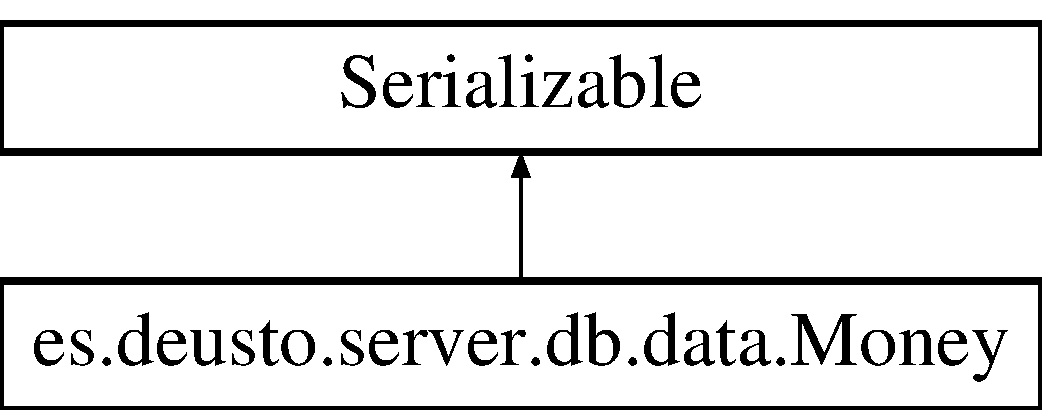
\includegraphics[height=2.000000cm]{classes_1_1deusto_1_1server_1_1db_1_1data_1_1_money}
\end{center}
\end{figure}
\subsection*{Public Member Functions}
\begin{DoxyCompactItemize}
\item 
\hyperlink{classes_1_1deusto_1_1server_1_1db_1_1data_1_1_money_a25df7b8a67c257434bf09b7d8e7e2dbd}{Money} (int amount)
\item 
\hyperlink{classes_1_1deusto_1_1server_1_1db_1_1data_1_1_user}{User} \hyperlink{classes_1_1deusto_1_1server_1_1db_1_1data_1_1_money_a4e51e8a920ff96f945c59693c7bf08ad}{get\+Sender} ()
\item 
\hyperlink{classes_1_1deusto_1_1server_1_1db_1_1data_1_1_product}{Product} \hyperlink{classes_1_1deusto_1_1server_1_1db_1_1data_1_1_money_ab907da0a2fa2c7d42034f323ff1d86a7}{get\+Prod} ()
\item 
void \hyperlink{classes_1_1deusto_1_1server_1_1db_1_1data_1_1_money_ad5e5b686cbe1ce6e631915f40ef70892}{set\+User\+Sending} (\hyperlink{classes_1_1deusto_1_1server_1_1db_1_1data_1_1_user}{User} sender)
\item 
void \hyperlink{classes_1_1deusto_1_1server_1_1db_1_1data_1_1_money_a494f3b9ca18e88ca4b96e9c8d90e0557}{set\+Product} (\hyperlink{classes_1_1deusto_1_1server_1_1db_1_1data_1_1_product}{Product} p)
\item 
int \hyperlink{classes_1_1deusto_1_1server_1_1db_1_1data_1_1_money_a6f9db9361544c72ecaa89ec27309645d}{get\+Amount} ()
\item 
String \hyperlink{classes_1_1deusto_1_1server_1_1db_1_1data_1_1_money_a97d3500731b427992e9e40dcc0f0442d}{to\+String} ()
\end{DoxyCompactItemize}


\subsection{Detailed Description}


Definition at line 13 of file Money.\+java.



\subsection{Constructor \& Destructor Documentation}
\mbox{\Hypertarget{classes_1_1deusto_1_1server_1_1db_1_1data_1_1_money_a25df7b8a67c257434bf09b7d8e7e2dbd}\label{classes_1_1deusto_1_1server_1_1db_1_1data_1_1_money_a25df7b8a67c257434bf09b7d8e7e2dbd}} 
\index{es\+::deusto\+::server\+::db\+::data\+::\+Money@{es\+::deusto\+::server\+::db\+::data\+::\+Money}!Money@{Money}}
\index{Money@{Money}!es\+::deusto\+::server\+::db\+::data\+::\+Money@{es\+::deusto\+::server\+::db\+::data\+::\+Money}}
\subsubsection{\texorpdfstring{Money()}{Money()}}
{\footnotesize\ttfamily es.\+deusto.\+server.\+db.\+data.\+Money.\+Money (\begin{DoxyParamCaption}\item[{int}]{amount }\end{DoxyParamCaption})}

Method to create a new instance of an object \hyperlink{classes_1_1deusto_1_1server_1_1db_1_1data_1_1_product}{Product} 
\begin{DoxyParams}{Parameters}
{\em amount} & establishes the value for the parameter amount \\
\hline
\end{DoxyParams}


Definition at line 28 of file Money.\+java.



\subsection{Member Function Documentation}
\mbox{\Hypertarget{classes_1_1deusto_1_1server_1_1db_1_1data_1_1_money_a6f9db9361544c72ecaa89ec27309645d}\label{classes_1_1deusto_1_1server_1_1db_1_1data_1_1_money_a6f9db9361544c72ecaa89ec27309645d}} 
\index{es\+::deusto\+::server\+::db\+::data\+::\+Money@{es\+::deusto\+::server\+::db\+::data\+::\+Money}!get\+Amount@{get\+Amount}}
\index{get\+Amount@{get\+Amount}!es\+::deusto\+::server\+::db\+::data\+::\+Money@{es\+::deusto\+::server\+::db\+::data\+::\+Money}}
\subsubsection{\texorpdfstring{get\+Amount()}{getAmount()}}
{\footnotesize\ttfamily int es.\+deusto.\+server.\+db.\+data.\+Money.\+get\+Amount (\begin{DoxyParamCaption}{ }\end{DoxyParamCaption})}

This method returns the amount of the money \begin{DoxyReturn}{Returns}
The amount of money in the interaction 
\end{DoxyReturn}


Definition at line 69 of file Money.\+java.

\mbox{\Hypertarget{classes_1_1deusto_1_1server_1_1db_1_1data_1_1_money_ab907da0a2fa2c7d42034f323ff1d86a7}\label{classes_1_1deusto_1_1server_1_1db_1_1data_1_1_money_ab907da0a2fa2c7d42034f323ff1d86a7}} 
\index{es\+::deusto\+::server\+::db\+::data\+::\+Money@{es\+::deusto\+::server\+::db\+::data\+::\+Money}!get\+Prod@{get\+Prod}}
\index{get\+Prod@{get\+Prod}!es\+::deusto\+::server\+::db\+::data\+::\+Money@{es\+::deusto\+::server\+::db\+::data\+::\+Money}}
\subsubsection{\texorpdfstring{get\+Prod()}{getProd()}}
{\footnotesize\ttfamily \hyperlink{classes_1_1deusto_1_1server_1_1db_1_1data_1_1_product}{Product} es.\+deusto.\+server.\+db.\+data.\+Money.\+get\+Prod (\begin{DoxyParamCaption}{ }\end{DoxyParamCaption})}

This method returns the product inside the money interaction \begin{DoxyReturn}{Returns}
The product of the money interaction 
\end{DoxyReturn}


Definition at line 45 of file Money.\+java.

\mbox{\Hypertarget{classes_1_1deusto_1_1server_1_1db_1_1data_1_1_money_a4e51e8a920ff96f945c59693c7bf08ad}\label{classes_1_1deusto_1_1server_1_1db_1_1data_1_1_money_a4e51e8a920ff96f945c59693c7bf08ad}} 
\index{es\+::deusto\+::server\+::db\+::data\+::\+Money@{es\+::deusto\+::server\+::db\+::data\+::\+Money}!get\+Sender@{get\+Sender}}
\index{get\+Sender@{get\+Sender}!es\+::deusto\+::server\+::db\+::data\+::\+Money@{es\+::deusto\+::server\+::db\+::data\+::\+Money}}
\subsubsection{\texorpdfstring{get\+Sender()}{getSender()}}
{\footnotesize\ttfamily \hyperlink{classes_1_1deusto_1_1server_1_1db_1_1data_1_1_user}{User} es.\+deusto.\+server.\+db.\+data.\+Money.\+get\+Sender (\begin{DoxyParamCaption}{ }\end{DoxyParamCaption})}

This method returns the user that sends the money \begin{DoxyReturn}{Returns}
The sender of the money 
\end{DoxyReturn}


Definition at line 37 of file Money.\+java.

\mbox{\Hypertarget{classes_1_1deusto_1_1server_1_1db_1_1data_1_1_money_a494f3b9ca18e88ca4b96e9c8d90e0557}\label{classes_1_1deusto_1_1server_1_1db_1_1data_1_1_money_a494f3b9ca18e88ca4b96e9c8d90e0557}} 
\index{es\+::deusto\+::server\+::db\+::data\+::\+Money@{es\+::deusto\+::server\+::db\+::data\+::\+Money}!set\+Product@{set\+Product}}
\index{set\+Product@{set\+Product}!es\+::deusto\+::server\+::db\+::data\+::\+Money@{es\+::deusto\+::server\+::db\+::data\+::\+Money}}
\subsubsection{\texorpdfstring{set\+Product()}{setProduct()}}
{\footnotesize\ttfamily void es.\+deusto.\+server.\+db.\+data.\+Money.\+set\+Product (\begin{DoxyParamCaption}\item[{\hyperlink{classes_1_1deusto_1_1server_1_1db_1_1data_1_1_product}{Product}}]{p }\end{DoxyParamCaption})}

Establishes the value for the parameter sender of the \hyperlink{classes_1_1deusto_1_1server_1_1db_1_1data_1_1_money}{Money} 
\begin{DoxyParams}{Parameters}
{\em p} & the product inside the money interaction \\
\hline
\end{DoxyParams}


Definition at line 61 of file Money.\+java.

\mbox{\Hypertarget{classes_1_1deusto_1_1server_1_1db_1_1data_1_1_money_ad5e5b686cbe1ce6e631915f40ef70892}\label{classes_1_1deusto_1_1server_1_1db_1_1data_1_1_money_ad5e5b686cbe1ce6e631915f40ef70892}} 
\index{es\+::deusto\+::server\+::db\+::data\+::\+Money@{es\+::deusto\+::server\+::db\+::data\+::\+Money}!set\+User\+Sending@{set\+User\+Sending}}
\index{set\+User\+Sending@{set\+User\+Sending}!es\+::deusto\+::server\+::db\+::data\+::\+Money@{es\+::deusto\+::server\+::db\+::data\+::\+Money}}
\subsubsection{\texorpdfstring{set\+User\+Sending()}{setUserSending()}}
{\footnotesize\ttfamily void es.\+deusto.\+server.\+db.\+data.\+Money.\+set\+User\+Sending (\begin{DoxyParamCaption}\item[{\hyperlink{classes_1_1deusto_1_1server_1_1db_1_1data_1_1_user}{User}}]{sender }\end{DoxyParamCaption})}

Establishes the value for the parameter sender of the \hyperlink{classes_1_1deusto_1_1server_1_1db_1_1data_1_1_money}{Money} 
\begin{DoxyParams}{Parameters}
{\em sender} & the user that will send the money \\
\hline
\end{DoxyParams}


Definition at line 53 of file Money.\+java.

\mbox{\Hypertarget{classes_1_1deusto_1_1server_1_1db_1_1data_1_1_money_a97d3500731b427992e9e40dcc0f0442d}\label{classes_1_1deusto_1_1server_1_1db_1_1data_1_1_money_a97d3500731b427992e9e40dcc0f0442d}} 
\index{es\+::deusto\+::server\+::db\+::data\+::\+Money@{es\+::deusto\+::server\+::db\+::data\+::\+Money}!to\+String@{to\+String}}
\index{to\+String@{to\+String}!es\+::deusto\+::server\+::db\+::data\+::\+Money@{es\+::deusto\+::server\+::db\+::data\+::\+Money}}
\subsubsection{\texorpdfstring{to\+String()}{toString()}}
{\footnotesize\ttfamily String es.\+deusto.\+server.\+db.\+data.\+Money.\+to\+String (\begin{DoxyParamCaption}{ }\end{DoxyParamCaption})}



Definition at line 71 of file Money.\+java.



The documentation for this class was generated from the following file\+:\begin{DoxyCompactItemize}
\item 
C\+:/\+Users/\+Oihane/git/\+S\+P\+Q03/spq03/src/main/java/es/deusto/server/db/data/\hyperlink{_money_8java}{Money.\+java}\end{DoxyCompactItemize}

\hypertarget{classes_1_1deusto_1_1client_1_1_new_prod_window}{}\section{es.\+deusto.\+client.\+New\+Prod\+Window Class Reference}
\label{classes_1_1deusto_1_1client_1_1_new_prod_window}\index{es.\+deusto.\+client.\+New\+Prod\+Window@{es.\+deusto.\+client.\+New\+Prod\+Window}}
Inheritance diagram for es.\+deusto.\+client.\+New\+Prod\+Window\+:\begin{figure}[H]
\begin{center}
\leavevmode
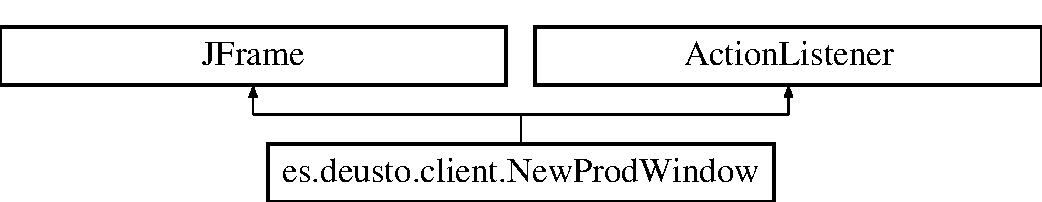
\includegraphics[height=2.000000cm]{classes_1_1deusto_1_1client_1_1_new_prod_window}
\end{center}
\end{figure}
\subsection*{Public Member Functions}
\begin{DoxyCompactItemize}
\item 
\hyperlink{classes_1_1deusto_1_1client_1_1_new_prod_window_a07ce756a81d6cf22bfc218ce374a7dfb}{New\+Prod\+Window} ()
\item 
void \hyperlink{classes_1_1deusto_1_1client_1_1_new_prod_window_a55a477c0bf87e25c575b47ffecc34d5f}{action\+Performed} (Action\+Event e)
\item 
void \hyperlink{classes_1_1deusto_1_1client_1_1_new_prod_window_aa254d28487576c4a20e270fa24bdf384}{set\+Transferer} (\hyperlink{interfacees_1_1deusto_1_1server_1_1remote_1_1_i_transferer}{I\+Transferer} i\+Trans)
\end{DoxyCompactItemize}


\subsection{Detailed Description}


Definition at line 21 of file New\+Prod\+Window.\+java.



\subsection{Constructor \& Destructor Documentation}
\mbox{\Hypertarget{classes_1_1deusto_1_1client_1_1_new_prod_window_a07ce756a81d6cf22bfc218ce374a7dfb}\label{classes_1_1deusto_1_1client_1_1_new_prod_window_a07ce756a81d6cf22bfc218ce374a7dfb}} 
\index{es\+::deusto\+::client\+::\+New\+Prod\+Window@{es\+::deusto\+::client\+::\+New\+Prod\+Window}!New\+Prod\+Window@{New\+Prod\+Window}}
\index{New\+Prod\+Window@{New\+Prod\+Window}!es\+::deusto\+::client\+::\+New\+Prod\+Window@{es\+::deusto\+::client\+::\+New\+Prod\+Window}}
\subsubsection{\texorpdfstring{New\+Prod\+Window()}{NewProdWindow()}}
{\footnotesize\ttfamily es.\+deusto.\+client.\+New\+Prod\+Window.\+New\+Prod\+Window (\begin{DoxyParamCaption}{ }\end{DoxyParamCaption})}



Definition at line 31 of file New\+Prod\+Window.\+java.



\subsection{Member Function Documentation}
\mbox{\Hypertarget{classes_1_1deusto_1_1client_1_1_new_prod_window_a55a477c0bf87e25c575b47ffecc34d5f}\label{classes_1_1deusto_1_1client_1_1_new_prod_window_a55a477c0bf87e25c575b47ffecc34d5f}} 
\index{es\+::deusto\+::client\+::\+New\+Prod\+Window@{es\+::deusto\+::client\+::\+New\+Prod\+Window}!action\+Performed@{action\+Performed}}
\index{action\+Performed@{action\+Performed}!es\+::deusto\+::client\+::\+New\+Prod\+Window@{es\+::deusto\+::client\+::\+New\+Prod\+Window}}
\subsubsection{\texorpdfstring{action\+Performed()}{actionPerformed()}}
{\footnotesize\ttfamily void es.\+deusto.\+client.\+New\+Prod\+Window.\+action\+Performed (\begin{DoxyParamCaption}\item[{Action\+Event}]{e }\end{DoxyParamCaption})}



Definition at line 70 of file New\+Prod\+Window.\+java.

\mbox{\Hypertarget{classes_1_1deusto_1_1client_1_1_new_prod_window_aa254d28487576c4a20e270fa24bdf384}\label{classes_1_1deusto_1_1client_1_1_new_prod_window_aa254d28487576c4a20e270fa24bdf384}} 
\index{es\+::deusto\+::client\+::\+New\+Prod\+Window@{es\+::deusto\+::client\+::\+New\+Prod\+Window}!set\+Transferer@{set\+Transferer}}
\index{set\+Transferer@{set\+Transferer}!es\+::deusto\+::client\+::\+New\+Prod\+Window@{es\+::deusto\+::client\+::\+New\+Prod\+Window}}
\subsubsection{\texorpdfstring{set\+Transferer()}{setTransferer()}}
{\footnotesize\ttfamily void es.\+deusto.\+client.\+New\+Prod\+Window.\+set\+Transferer (\begin{DoxyParamCaption}\item[{\hyperlink{interfacees_1_1deusto_1_1server_1_1remote_1_1_i_transferer}{I\+Transferer}}]{i\+Trans }\end{DoxyParamCaption})}



Definition at line 87 of file New\+Prod\+Window.\+java.



The documentation for this class was generated from the following file\+:\begin{DoxyCompactItemize}
\item 
C\+:/\+Users/\+Oihane/git/\+S\+P\+Q03/spq03/src/main/java/es/deusto/client/\hyperlink{_new_prod_window_8java}{New\+Prod\+Window.\+java}\end{DoxyCompactItemize}

\hypertarget{classes_1_1deusto_1_1server_1_1db_1_1data_1_1_product}{}\section{es.\+deusto.\+server.\+db.\+data.\+Product Class Reference}
\label{classes_1_1deusto_1_1server_1_1db_1_1data_1_1_product}\index{es.\+deusto.\+server.\+db.\+data.\+Product@{es.\+deusto.\+server.\+db.\+data.\+Product}}
Inheritance diagram for es.\+deusto.\+server.\+db.\+data.\+Product\+:\begin{figure}[H]
\begin{center}
\leavevmode
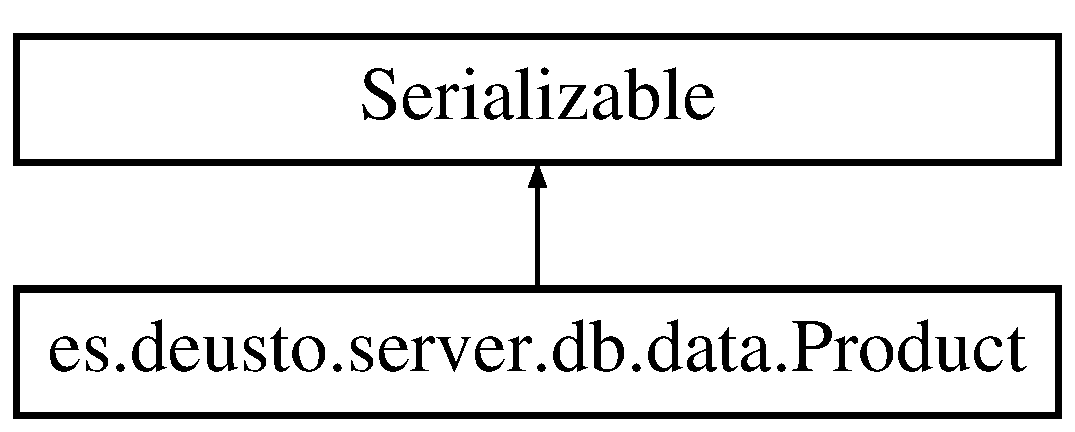
\includegraphics[height=2.000000cm]{classes_1_1deusto_1_1server_1_1db_1_1data_1_1_product}
\end{center}
\end{figure}
\subsection*{Public Member Functions}
\begin{DoxyCompactItemize}
\item 
\hyperlink{classes_1_1deusto_1_1server_1_1db_1_1data_1_1_product_a8c697db6ce4cede760ae565dfde3ac3e}{Product} (String name, String characteristics)
\item 
\hyperlink{classes_1_1deusto_1_1server_1_1db_1_1data_1_1_user}{User} \hyperlink{classes_1_1deusto_1_1server_1_1db_1_1data_1_1_product_a2e60d68bada56d93ec2ef5e67a0c3d9f}{dn\+Getuser} ()
\item 
String \hyperlink{classes_1_1deusto_1_1server_1_1db_1_1data_1_1_product_a140ac892e13b36b2c6da61b3abb06f4e}{get\+Name} ()
\item 
void \hyperlink{classes_1_1deusto_1_1server_1_1db_1_1data_1_1_product_a68feb5bdb4b611fecd9c07eee9217ac6}{set\+Name} (String name)
\item 
void \hyperlink{classes_1_1deusto_1_1server_1_1db_1_1data_1_1_product_a72a7c230f6309248b5f6e6027189c996}{set\+Owner} (\hyperlink{classes_1_1deusto_1_1server_1_1db_1_1data_1_1_user}{User} owner)
\item 
String \hyperlink{classes_1_1deusto_1_1server_1_1db_1_1data_1_1_product_ab352b5efab8c748a45e8d28b9fad2411}{get\+Characteristics} ()
\item 
String \hyperlink{classes_1_1deusto_1_1server_1_1db_1_1data_1_1_product_a486ece3e8cc4e08b086239c0ea11b492}{get\+Buyers\+Payment} ()
\item 
String \hyperlink{classes_1_1deusto_1_1server_1_1db_1_1data_1_1_product_a4cc3da392d5679515cd8da38f88bc920}{to\+String} ()
\item 
String \hyperlink{classes_1_1deusto_1_1server_1_1db_1_1data_1_1_product_ada09de3915be881fe42f6f61bfd048f8}{to\+String\+Short} ()
\end{DoxyCompactItemize}


\subsection{Detailed Description}


Definition at line 18 of file Product.\+java.



\subsection{Constructor \& Destructor Documentation}
\mbox{\Hypertarget{classes_1_1deusto_1_1server_1_1db_1_1data_1_1_product_a8c697db6ce4cede760ae565dfde3ac3e}\label{classes_1_1deusto_1_1server_1_1db_1_1data_1_1_product_a8c697db6ce4cede760ae565dfde3ac3e}} 
\index{es\+::deusto\+::server\+::db\+::data\+::\+Product@{es\+::deusto\+::server\+::db\+::data\+::\+Product}!Product@{Product}}
\index{Product@{Product}!es\+::deusto\+::server\+::db\+::data\+::\+Product@{es\+::deusto\+::server\+::db\+::data\+::\+Product}}
\subsubsection{\texorpdfstring{Product()}{Product()}}
{\footnotesize\ttfamily es.\+deusto.\+server.\+db.\+data.\+Product.\+Product (\begin{DoxyParamCaption}\item[{String}]{name,  }\item[{String}]{characteristics }\end{DoxyParamCaption})}

Method to create a new instance of an object \hyperlink{classes_1_1deusto_1_1server_1_1db_1_1data_1_1_product}{Product} 
\begin{DoxyParams}{Parameters}
{\em name} & The value for the PK that will identify a product between all the ones in the \hyperlink{classes_1_1deusto_1_1server_1_1db_1_1_d_b}{DB} \\
\hline
{\em characteristics} & The value for the characteristics of the product \\
\hline
\end{DoxyParams}


Definition at line 40 of file Product.\+java.



\subsection{Member Function Documentation}
\mbox{\Hypertarget{classes_1_1deusto_1_1server_1_1db_1_1data_1_1_product_a2e60d68bada56d93ec2ef5e67a0c3d9f}\label{classes_1_1deusto_1_1server_1_1db_1_1data_1_1_product_a2e60d68bada56d93ec2ef5e67a0c3d9f}} 
\index{es\+::deusto\+::server\+::db\+::data\+::\+Product@{es\+::deusto\+::server\+::db\+::data\+::\+Product}!dn\+Getuser@{dn\+Getuser}}
\index{dn\+Getuser@{dn\+Getuser}!es\+::deusto\+::server\+::db\+::data\+::\+Product@{es\+::deusto\+::server\+::db\+::data\+::\+Product}}
\subsubsection{\texorpdfstring{dn\+Getuser()}{dnGetuser()}}
{\footnotesize\ttfamily \hyperlink{classes_1_1deusto_1_1server_1_1db_1_1data_1_1_user}{User} es.\+deusto.\+server.\+db.\+data.\+Product.\+dn\+Getuser (\begin{DoxyParamCaption}{ }\end{DoxyParamCaption})}

This method returns the user that owns the product \begin{DoxyReturn}{Returns}
The owner of the \hyperlink{classes_1_1deusto_1_1server_1_1db_1_1data_1_1_product}{Product} 
\end{DoxyReturn}


Definition at line 50 of file Product.\+java.

\mbox{\Hypertarget{classes_1_1deusto_1_1server_1_1db_1_1data_1_1_product_a486ece3e8cc4e08b086239c0ea11b492}\label{classes_1_1deusto_1_1server_1_1db_1_1data_1_1_product_a486ece3e8cc4e08b086239c0ea11b492}} 
\index{es\+::deusto\+::server\+::db\+::data\+::\+Product@{es\+::deusto\+::server\+::db\+::data\+::\+Product}!get\+Buyers\+Payment@{get\+Buyers\+Payment}}
\index{get\+Buyers\+Payment@{get\+Buyers\+Payment}!es\+::deusto\+::server\+::db\+::data\+::\+Product@{es\+::deusto\+::server\+::db\+::data\+::\+Product}}
\subsubsection{\texorpdfstring{get\+Buyers\+Payment()}{getBuyersPayment()}}
{\footnotesize\ttfamily String es.\+deusto.\+server.\+db.\+data.\+Product.\+get\+Buyers\+Payment (\begin{DoxyParamCaption}{ }\end{DoxyParamCaption})}

This method returns the buyers payment of the product \begin{DoxyReturn}{Returns}
The buyers payment of the \hyperlink{classes_1_1deusto_1_1server_1_1db_1_1data_1_1_product}{Product} 
\end{DoxyReturn}


Definition at line 86 of file Product.\+java.

\mbox{\Hypertarget{classes_1_1deusto_1_1server_1_1db_1_1data_1_1_product_ab352b5efab8c748a45e8d28b9fad2411}\label{classes_1_1deusto_1_1server_1_1db_1_1data_1_1_product_ab352b5efab8c748a45e8d28b9fad2411}} 
\index{es\+::deusto\+::server\+::db\+::data\+::\+Product@{es\+::deusto\+::server\+::db\+::data\+::\+Product}!get\+Characteristics@{get\+Characteristics}}
\index{get\+Characteristics@{get\+Characteristics}!es\+::deusto\+::server\+::db\+::data\+::\+Product@{es\+::deusto\+::server\+::db\+::data\+::\+Product}}
\subsubsection{\texorpdfstring{get\+Characteristics()}{getCharacteristics()}}
{\footnotesize\ttfamily String es.\+deusto.\+server.\+db.\+data.\+Product.\+get\+Characteristics (\begin{DoxyParamCaption}{ }\end{DoxyParamCaption})}

This method returns the characteristics of the product \begin{DoxyReturn}{Returns}
The characteristics of the \hyperlink{classes_1_1deusto_1_1server_1_1db_1_1data_1_1_product}{Product} 
\end{DoxyReturn}


Definition at line 80 of file Product.\+java.

\mbox{\Hypertarget{classes_1_1deusto_1_1server_1_1db_1_1data_1_1_product_a140ac892e13b36b2c6da61b3abb06f4e}\label{classes_1_1deusto_1_1server_1_1db_1_1data_1_1_product_a140ac892e13b36b2c6da61b3abb06f4e}} 
\index{es\+::deusto\+::server\+::db\+::data\+::\+Product@{es\+::deusto\+::server\+::db\+::data\+::\+Product}!get\+Name@{get\+Name}}
\index{get\+Name@{get\+Name}!es\+::deusto\+::server\+::db\+::data\+::\+Product@{es\+::deusto\+::server\+::db\+::data\+::\+Product}}
\subsubsection{\texorpdfstring{get\+Name()}{getName()}}
{\footnotesize\ttfamily String es.\+deusto.\+server.\+db.\+data.\+Product.\+get\+Name (\begin{DoxyParamCaption}{ }\end{DoxyParamCaption})}

This method returns the name (PK) of the product \begin{DoxyReturn}{Returns}
The name of the \hyperlink{classes_1_1deusto_1_1server_1_1db_1_1data_1_1_product}{Product} 
\end{DoxyReturn}


Definition at line 58 of file Product.\+java.

\mbox{\Hypertarget{classes_1_1deusto_1_1server_1_1db_1_1data_1_1_product_a68feb5bdb4b611fecd9c07eee9217ac6}\label{classes_1_1deusto_1_1server_1_1db_1_1data_1_1_product_a68feb5bdb4b611fecd9c07eee9217ac6}} 
\index{es\+::deusto\+::server\+::db\+::data\+::\+Product@{es\+::deusto\+::server\+::db\+::data\+::\+Product}!set\+Name@{set\+Name}}
\index{set\+Name@{set\+Name}!es\+::deusto\+::server\+::db\+::data\+::\+Product@{es\+::deusto\+::server\+::db\+::data\+::\+Product}}
\subsubsection{\texorpdfstring{set\+Name()}{setName()}}
{\footnotesize\ttfamily void es.\+deusto.\+server.\+db.\+data.\+Product.\+set\+Name (\begin{DoxyParamCaption}\item[{String}]{name }\end{DoxyParamCaption})}

Establishes the value for the parameter name of the \hyperlink{classes_1_1deusto_1_1server_1_1db_1_1data_1_1_product}{Product} 
\begin{DoxyParams}{Parameters}
{\em name} & The value for the name \\
\hline
\end{DoxyParams}


Definition at line 66 of file Product.\+java.

\mbox{\Hypertarget{classes_1_1deusto_1_1server_1_1db_1_1data_1_1_product_a72a7c230f6309248b5f6e6027189c996}\label{classes_1_1deusto_1_1server_1_1db_1_1data_1_1_product_a72a7c230f6309248b5f6e6027189c996}} 
\index{es\+::deusto\+::server\+::db\+::data\+::\+Product@{es\+::deusto\+::server\+::db\+::data\+::\+Product}!set\+Owner@{set\+Owner}}
\index{set\+Owner@{set\+Owner}!es\+::deusto\+::server\+::db\+::data\+::\+Product@{es\+::deusto\+::server\+::db\+::data\+::\+Product}}
\subsubsection{\texorpdfstring{set\+Owner()}{setOwner()}}
{\footnotesize\ttfamily void es.\+deusto.\+server.\+db.\+data.\+Product.\+set\+Owner (\begin{DoxyParamCaption}\item[{\hyperlink{classes_1_1deusto_1_1server_1_1db_1_1data_1_1_user}{User}}]{owner }\end{DoxyParamCaption})}

Establishes the value for the parameter owner of the \hyperlink{classes_1_1deusto_1_1server_1_1db_1_1data_1_1_product}{Product} 
\begin{DoxyParams}{Parameters}
{\em owner} & The value for the new owner \\
\hline
\end{DoxyParams}


Definition at line 72 of file Product.\+java.

\mbox{\Hypertarget{classes_1_1deusto_1_1server_1_1db_1_1data_1_1_product_a4cc3da392d5679515cd8da38f88bc920}\label{classes_1_1deusto_1_1server_1_1db_1_1data_1_1_product_a4cc3da392d5679515cd8da38f88bc920}} 
\index{es\+::deusto\+::server\+::db\+::data\+::\+Product@{es\+::deusto\+::server\+::db\+::data\+::\+Product}!to\+String@{to\+String}}
\index{to\+String@{to\+String}!es\+::deusto\+::server\+::db\+::data\+::\+Product@{es\+::deusto\+::server\+::db\+::data\+::\+Product}}
\subsubsection{\texorpdfstring{to\+String()}{toString()}}
{\footnotesize\ttfamily String es.\+deusto.\+server.\+db.\+data.\+Product.\+to\+String (\begin{DoxyParamCaption}{ }\end{DoxyParamCaption})}



Definition at line 94 of file Product.\+java.

\mbox{\Hypertarget{classes_1_1deusto_1_1server_1_1db_1_1data_1_1_product_ada09de3915be881fe42f6f61bfd048f8}\label{classes_1_1deusto_1_1server_1_1db_1_1data_1_1_product_ada09de3915be881fe42f6f61bfd048f8}} 
\index{es\+::deusto\+::server\+::db\+::data\+::\+Product@{es\+::deusto\+::server\+::db\+::data\+::\+Product}!to\+String\+Short@{to\+String\+Short}}
\index{to\+String\+Short@{to\+String\+Short}!es\+::deusto\+::server\+::db\+::data\+::\+Product@{es\+::deusto\+::server\+::db\+::data\+::\+Product}}
\subsubsection{\texorpdfstring{to\+String\+Short()}{toStringShort()}}
{\footnotesize\ttfamily String es.\+deusto.\+server.\+db.\+data.\+Product.\+to\+String\+Short (\begin{DoxyParamCaption}{ }\end{DoxyParamCaption})}



Definition at line 98 of file Product.\+java.



The documentation for this class was generated from the following file\+:\begin{DoxyCompactItemize}
\item 
C\+:/\+Users/\+Oihane/git/\+S\+P\+Q03/spq03/src/main/java/es/deusto/server/db/data/\hyperlink{_product_8java}{Product.\+java}\end{DoxyCompactItemize}

\hypertarget{classes_1_1deusto_1_1server_1_1_server}{}\section{es.\+deusto.\+server.\+Server Class Reference}
\label{classes_1_1deusto_1_1server_1_1_server}\index{es.\+deusto.\+server.\+Server@{es.\+deusto.\+server.\+Server}}
\subsection*{Static Public Member Functions}
\begin{DoxyCompactItemize}
\item 
static void \hyperlink{classes_1_1deusto_1_1server_1_1_server_a750bb0d7dbd89246a3602f2e20d03fb5}{main} (String\mbox{[}$\,$\mbox{]} args)
\end{DoxyCompactItemize}


\subsection{Detailed Description}


Definition at line 16 of file Server.\+java.



\subsection{Member Function Documentation}
\mbox{\Hypertarget{classes_1_1deusto_1_1server_1_1_server_a750bb0d7dbd89246a3602f2e20d03fb5}\label{classes_1_1deusto_1_1server_1_1_server_a750bb0d7dbd89246a3602f2e20d03fb5}} 
\index{es\+::deusto\+::server\+::\+Server@{es\+::deusto\+::server\+::\+Server}!main@{main}}
\index{main@{main}!es\+::deusto\+::server\+::\+Server@{es\+::deusto\+::server\+::\+Server}}
\subsubsection{\texorpdfstring{main()}{main()}}
{\footnotesize\ttfamily static void es.\+deusto.\+server.\+Server.\+main (\begin{DoxyParamCaption}\item[{String \mbox{[}$\,$\mbox{]}}]{args }\end{DoxyParamCaption})\hspace{0.3cm}{\ttfamily [static]}}



Definition at line 19 of file Server.\+java.



The documentation for this class was generated from the following file\+:\begin{DoxyCompactItemize}
\item 
C\+:/\+Users/\+Oihane/git/\+S\+P\+Q03/spq03/src/main/java/es/deusto/server/\hyperlink{_server_8java}{Server.\+java}\end{DoxyCompactItemize}

\hypertarget{classes_1_1deusto_1_1server_1_1remote_1_1_transferer}{}\section{es.\+deusto.\+server.\+remote.\+Transferer Class Reference}
\label{classes_1_1deusto_1_1server_1_1remote_1_1_transferer}\index{es.\+deusto.\+server.\+remote.\+Transferer@{es.\+deusto.\+server.\+remote.\+Transferer}}
Inheritance diagram for es.\+deusto.\+server.\+remote.\+Transferer\+:\begin{figure}[H]
\begin{center}
\leavevmode
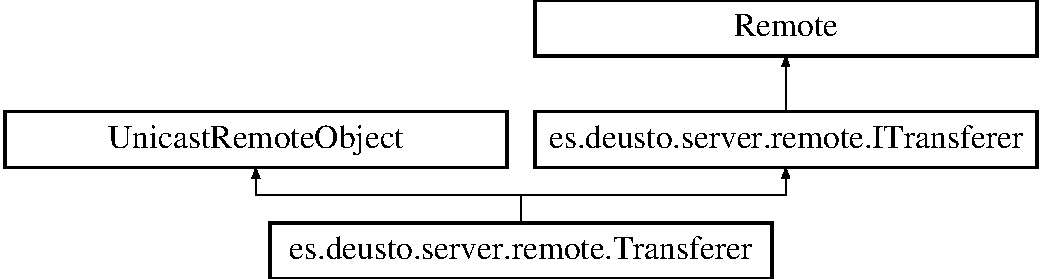
\includegraphics[height=3.000000cm]{classes_1_1deusto_1_1server_1_1remote_1_1_transferer}
\end{center}
\end{figure}
\subsection*{Public Member Functions}
\begin{DoxyCompactItemize}
\item 
\hyperlink{classes_1_1deusto_1_1server_1_1remote_1_1_transferer_ad9465ee99430add24c3bf6badab21a91}{Transferer} ()  throws Remote\+Exception 
\item 
\hyperlink{classes_1_1deusto_1_1server_1_1remote_1_1_transferer_a1cd1f321e0f5650f8a37907e8cb23840}{Transferer} (\hyperlink{interfacees_1_1deusto_1_1server_1_1db_1_1dao_1_1_i_d_a_o}{I\+D\+AO} udao)  throws Remote\+Exception 
\item 
Array\+List$<$ \hyperlink{classes_1_1deusto_1_1server_1_1db_1_1data_1_1_user}{User} $>$ \hyperlink{classes_1_1deusto_1_1server_1_1remote_1_1_transferer_a613c0c3af149140e58488ce9d0745593}{get\+All\+User} ()  throws Remote\+Exception
\item 
boolean \hyperlink{classes_1_1deusto_1_1server_1_1remote_1_1_transferer_a80e2dd7db595bdd8d39969e5d0e8ae7b}{register\+User} (\hyperlink{classes_1_1deusto_1_1server_1_1db_1_1data_1_1_user}{User} u)
\item 
\hyperlink{classes_1_1deusto_1_1server_1_1db_1_1data_1_1_user}{User} \hyperlink{classes_1_1deusto_1_1server_1_1remote_1_1_transferer_a16976959aeb3080244422aeac061a23b}{get\+User} (String login)  throws Remote\+Exception
\item 
Array\+List$<$ \hyperlink{classes_1_1deusto_1_1server_1_1db_1_1data_1_1_product}{Product} $>$ \hyperlink{classes_1_1deusto_1_1server_1_1remote_1_1_transferer_a29cbb75edeb4e0973780fd379ef2b3fb}{get\+All\+Prod} ()  throws Remote\+Exception
\item 
\hyperlink{classes_1_1deusto_1_1server_1_1db_1_1data_1_1_product}{Product} \hyperlink{classes_1_1deusto_1_1server_1_1remote_1_1_transferer_ad6759f696eddd682b750f92ec41d1fcb}{search\+Prod} (String name)  throws Remote\+Exception
\item 
boolean \hyperlink{classes_1_1deusto_1_1server_1_1remote_1_1_transferer_a64c1f3b57b74106df83335b124937afe}{register\+Prod} (\hyperlink{classes_1_1deusto_1_1server_1_1db_1_1data_1_1_product}{Product} p)  throws Remote\+Exception
\item 
boolean \hyperlink{classes_1_1deusto_1_1server_1_1remote_1_1_transferer_ad5868dd67ee9a53e7cdf0c30e08a3a1b}{buy\+Prod} (String loginB, \hyperlink{classes_1_1deusto_1_1server_1_1db_1_1data_1_1_product}{Product} p, int amount, String loginS)  throws Remote\+Exception
\item 
boolean \hyperlink{classes_1_1deusto_1_1server_1_1remote_1_1_transferer_ad1eb84155ba0c457645f2ad53725320d}{send\+Money} (String loginR, int amount, String loginS)  throws Remote\+Exception 
\end{DoxyCompactItemize}


\subsection{Detailed Description}


Definition at line 15 of file Transferer.\+java.



\subsection{Constructor \& Destructor Documentation}
\mbox{\Hypertarget{classes_1_1deusto_1_1server_1_1remote_1_1_transferer_ad9465ee99430add24c3bf6badab21a91}\label{classes_1_1deusto_1_1server_1_1remote_1_1_transferer_ad9465ee99430add24c3bf6badab21a91}} 
\index{es\+::deusto\+::server\+::remote\+::\+Transferer@{es\+::deusto\+::server\+::remote\+::\+Transferer}!Transferer@{Transferer}}
\index{Transferer@{Transferer}!es\+::deusto\+::server\+::remote\+::\+Transferer@{es\+::deusto\+::server\+::remote\+::\+Transferer}}
\subsubsection{\texorpdfstring{Transferer()}{Transferer()}\hspace{0.1cm}{\footnotesize\ttfamily [1/2]}}
{\footnotesize\ttfamily es.\+deusto.\+server.\+remote.\+Transferer.\+Transferer (\begin{DoxyParamCaption}{ }\end{DoxyParamCaption}) throws Remote\+Exception}



Definition at line 22 of file Transferer.\+java.

\mbox{\Hypertarget{classes_1_1deusto_1_1server_1_1remote_1_1_transferer_a1cd1f321e0f5650f8a37907e8cb23840}\label{classes_1_1deusto_1_1server_1_1remote_1_1_transferer_a1cd1f321e0f5650f8a37907e8cb23840}} 
\index{es\+::deusto\+::server\+::remote\+::\+Transferer@{es\+::deusto\+::server\+::remote\+::\+Transferer}!Transferer@{Transferer}}
\index{Transferer@{Transferer}!es\+::deusto\+::server\+::remote\+::\+Transferer@{es\+::deusto\+::server\+::remote\+::\+Transferer}}
\subsubsection{\texorpdfstring{Transferer()}{Transferer()}\hspace{0.1cm}{\footnotesize\ttfamily [2/2]}}
{\footnotesize\ttfamily es.\+deusto.\+server.\+remote.\+Transferer.\+Transferer (\begin{DoxyParamCaption}\item[{\hyperlink{interfacees_1_1deusto_1_1server_1_1db_1_1dao_1_1_i_d_a_o}{I\+D\+AO}}]{udao }\end{DoxyParamCaption}) throws Remote\+Exception}



Definition at line 27 of file Transferer.\+java.



\subsection{Member Function Documentation}
\mbox{\Hypertarget{classes_1_1deusto_1_1server_1_1remote_1_1_transferer_ad5868dd67ee9a53e7cdf0c30e08a3a1b}\label{classes_1_1deusto_1_1server_1_1remote_1_1_transferer_ad5868dd67ee9a53e7cdf0c30e08a3a1b}} 
\index{es\+::deusto\+::server\+::remote\+::\+Transferer@{es\+::deusto\+::server\+::remote\+::\+Transferer}!buy\+Prod@{buy\+Prod}}
\index{buy\+Prod@{buy\+Prod}!es\+::deusto\+::server\+::remote\+::\+Transferer@{es\+::deusto\+::server\+::remote\+::\+Transferer}}
\subsubsection{\texorpdfstring{buy\+Prod()}{buyProd()}}
{\footnotesize\ttfamily boolean es.\+deusto.\+server.\+remote.\+Transferer.\+buy\+Prod (\begin{DoxyParamCaption}\item[{String}]{loginB,  }\item[{\hyperlink{classes_1_1deusto_1_1server_1_1db_1_1data_1_1_product}{Product}}]{p,  }\item[{int}]{amount,  }\item[{String}]{loginS }\end{DoxyParamCaption}) throws Remote\+Exception}



Implements \hyperlink{interfacees_1_1deusto_1_1server_1_1remote_1_1_i_transferer_a86d92e8a78257551122807ae02259950}{es.\+deusto.\+server.\+remote.\+I\+Transferer}.



Definition at line 135 of file Transferer.\+java.

\mbox{\Hypertarget{classes_1_1deusto_1_1server_1_1remote_1_1_transferer_a29cbb75edeb4e0973780fd379ef2b3fb}\label{classes_1_1deusto_1_1server_1_1remote_1_1_transferer_a29cbb75edeb4e0973780fd379ef2b3fb}} 
\index{es\+::deusto\+::server\+::remote\+::\+Transferer@{es\+::deusto\+::server\+::remote\+::\+Transferer}!get\+All\+Prod@{get\+All\+Prod}}
\index{get\+All\+Prod@{get\+All\+Prod}!es\+::deusto\+::server\+::remote\+::\+Transferer@{es\+::deusto\+::server\+::remote\+::\+Transferer}}
\subsubsection{\texorpdfstring{get\+All\+Prod()}{getAllProd()}}
{\footnotesize\ttfamily Array\+List$<$\hyperlink{classes_1_1deusto_1_1server_1_1db_1_1data_1_1_product}{Product}$>$ es.\+deusto.\+server.\+remote.\+Transferer.\+get\+All\+Prod (\begin{DoxyParamCaption}{ }\end{DoxyParamCaption}) throws Remote\+Exception}



Implements \hyperlink{interfacees_1_1deusto_1_1server_1_1remote_1_1_i_transferer_a71afa6799122b3f09805f86d2e58fc23}{es.\+deusto.\+server.\+remote.\+I\+Transferer}.



Definition at line 82 of file Transferer.\+java.

\mbox{\Hypertarget{classes_1_1deusto_1_1server_1_1remote_1_1_transferer_a613c0c3af149140e58488ce9d0745593}\label{classes_1_1deusto_1_1server_1_1remote_1_1_transferer_a613c0c3af149140e58488ce9d0745593}} 
\index{es\+::deusto\+::server\+::remote\+::\+Transferer@{es\+::deusto\+::server\+::remote\+::\+Transferer}!get\+All\+User@{get\+All\+User}}
\index{get\+All\+User@{get\+All\+User}!es\+::deusto\+::server\+::remote\+::\+Transferer@{es\+::deusto\+::server\+::remote\+::\+Transferer}}
\subsubsection{\texorpdfstring{get\+All\+User()}{getAllUser()}}
{\footnotesize\ttfamily Array\+List$<$\hyperlink{classes_1_1deusto_1_1server_1_1db_1_1data_1_1_user}{User}$>$ es.\+deusto.\+server.\+remote.\+Transferer.\+get\+All\+User (\begin{DoxyParamCaption}{ }\end{DoxyParamCaption}) throws Remote\+Exception}



Implements \hyperlink{interfacees_1_1deusto_1_1server_1_1remote_1_1_i_transferer_aec6609427d773f075a78295a97888103}{es.\+deusto.\+server.\+remote.\+I\+Transferer}.



Definition at line 33 of file Transferer.\+java.

\mbox{\Hypertarget{classes_1_1deusto_1_1server_1_1remote_1_1_transferer_a16976959aeb3080244422aeac061a23b}\label{classes_1_1deusto_1_1server_1_1remote_1_1_transferer_a16976959aeb3080244422aeac061a23b}} 
\index{es\+::deusto\+::server\+::remote\+::\+Transferer@{es\+::deusto\+::server\+::remote\+::\+Transferer}!get\+User@{get\+User}}
\index{get\+User@{get\+User}!es\+::deusto\+::server\+::remote\+::\+Transferer@{es\+::deusto\+::server\+::remote\+::\+Transferer}}
\subsubsection{\texorpdfstring{get\+User()}{getUser()}}
{\footnotesize\ttfamily \hyperlink{classes_1_1deusto_1_1server_1_1db_1_1data_1_1_user}{User} es.\+deusto.\+server.\+remote.\+Transferer.\+get\+User (\begin{DoxyParamCaption}\item[{String}]{login }\end{DoxyParamCaption}) throws Remote\+Exception}



Implements \hyperlink{interfacees_1_1deusto_1_1server_1_1remote_1_1_i_transferer_ab767521556fc61bc5a39306080f00cae}{es.\+deusto.\+server.\+remote.\+I\+Transferer}.



Definition at line 65 of file Transferer.\+java.

\mbox{\Hypertarget{classes_1_1deusto_1_1server_1_1remote_1_1_transferer_a64c1f3b57b74106df83335b124937afe}\label{classes_1_1deusto_1_1server_1_1remote_1_1_transferer_a64c1f3b57b74106df83335b124937afe}} 
\index{es\+::deusto\+::server\+::remote\+::\+Transferer@{es\+::deusto\+::server\+::remote\+::\+Transferer}!register\+Prod@{register\+Prod}}
\index{register\+Prod@{register\+Prod}!es\+::deusto\+::server\+::remote\+::\+Transferer@{es\+::deusto\+::server\+::remote\+::\+Transferer}}
\subsubsection{\texorpdfstring{register\+Prod()}{registerProd()}}
{\footnotesize\ttfamily boolean es.\+deusto.\+server.\+remote.\+Transferer.\+register\+Prod (\begin{DoxyParamCaption}\item[{\hyperlink{classes_1_1deusto_1_1server_1_1db_1_1data_1_1_product}{Product}}]{p }\end{DoxyParamCaption}) throws Remote\+Exception}



Implements \hyperlink{interfacees_1_1deusto_1_1server_1_1remote_1_1_i_transferer_a06629c7021aae4d2ce1a449726102ded}{es.\+deusto.\+server.\+remote.\+I\+Transferer}.



Definition at line 113 of file Transferer.\+java.

\mbox{\Hypertarget{classes_1_1deusto_1_1server_1_1remote_1_1_transferer_a80e2dd7db595bdd8d39969e5d0e8ae7b}\label{classes_1_1deusto_1_1server_1_1remote_1_1_transferer_a80e2dd7db595bdd8d39969e5d0e8ae7b}} 
\index{es\+::deusto\+::server\+::remote\+::\+Transferer@{es\+::deusto\+::server\+::remote\+::\+Transferer}!register\+User@{register\+User}}
\index{register\+User@{register\+User}!es\+::deusto\+::server\+::remote\+::\+Transferer@{es\+::deusto\+::server\+::remote\+::\+Transferer}}
\subsubsection{\texorpdfstring{register\+User()}{registerUser()}}
{\footnotesize\ttfamily boolean es.\+deusto.\+server.\+remote.\+Transferer.\+register\+User (\begin{DoxyParamCaption}\item[{\hyperlink{classes_1_1deusto_1_1server_1_1db_1_1data_1_1_user}{User}}]{u }\end{DoxyParamCaption})}



Implements \hyperlink{interfacees_1_1deusto_1_1server_1_1remote_1_1_i_transferer_ab805207e578865de5bf2e69ca8942344}{es.\+deusto.\+server.\+remote.\+I\+Transferer}.



Definition at line 45 of file Transferer.\+java.

\mbox{\Hypertarget{classes_1_1deusto_1_1server_1_1remote_1_1_transferer_ad6759f696eddd682b750f92ec41d1fcb}\label{classes_1_1deusto_1_1server_1_1remote_1_1_transferer_ad6759f696eddd682b750f92ec41d1fcb}} 
\index{es\+::deusto\+::server\+::remote\+::\+Transferer@{es\+::deusto\+::server\+::remote\+::\+Transferer}!search\+Prod@{search\+Prod}}
\index{search\+Prod@{search\+Prod}!es\+::deusto\+::server\+::remote\+::\+Transferer@{es\+::deusto\+::server\+::remote\+::\+Transferer}}
\subsubsection{\texorpdfstring{search\+Prod()}{searchProd()}}
{\footnotesize\ttfamily \hyperlink{classes_1_1deusto_1_1server_1_1db_1_1data_1_1_product}{Product} es.\+deusto.\+server.\+remote.\+Transferer.\+search\+Prod (\begin{DoxyParamCaption}\item[{String}]{name }\end{DoxyParamCaption}) throws Remote\+Exception}



Implements \hyperlink{interfacees_1_1deusto_1_1server_1_1remote_1_1_i_transferer_a1fb33a5447e1647ffde8a01d180b8d99}{es.\+deusto.\+server.\+remote.\+I\+Transferer}.



Definition at line 94 of file Transferer.\+java.

\mbox{\Hypertarget{classes_1_1deusto_1_1server_1_1remote_1_1_transferer_ad1eb84155ba0c457645f2ad53725320d}\label{classes_1_1deusto_1_1server_1_1remote_1_1_transferer_ad1eb84155ba0c457645f2ad53725320d}} 
\index{es\+::deusto\+::server\+::remote\+::\+Transferer@{es\+::deusto\+::server\+::remote\+::\+Transferer}!send\+Money@{send\+Money}}
\index{send\+Money@{send\+Money}!es\+::deusto\+::server\+::remote\+::\+Transferer@{es\+::deusto\+::server\+::remote\+::\+Transferer}}
\subsubsection{\texorpdfstring{send\+Money()}{sendMoney()}}
{\footnotesize\ttfamily boolean es.\+deusto.\+server.\+remote.\+Transferer.\+send\+Money (\begin{DoxyParamCaption}\item[{String}]{loginR,  }\item[{int}]{amount,  }\item[{String}]{loginS }\end{DoxyParamCaption}) throws Remote\+Exception}



Implements \hyperlink{interfacees_1_1deusto_1_1server_1_1remote_1_1_i_transferer_ab43399cfce0d84f6e27032a7c14865f6}{es.\+deusto.\+server.\+remote.\+I\+Transferer}.



Definition at line 160 of file Transferer.\+java.



The documentation for this class was generated from the following file\+:\begin{DoxyCompactItemize}
\item 
C\+:/\+Users/\+Oihane/git/\+S\+P\+Q03/spq03/src/main/java/es/deusto/server/remote/\hyperlink{_transferer_8java}{Transferer.\+java}\end{DoxyCompactItemize}

\hypertarget{classes_1_1deusto_1_1server_1_1db_1_1data_1_1_user}{}\section{es.\+deusto.\+server.\+db.\+data.\+User Class Reference}
\label{classes_1_1deusto_1_1server_1_1db_1_1data_1_1_user}\index{es.\+deusto.\+server.\+db.\+data.\+User@{es.\+deusto.\+server.\+db.\+data.\+User}}
Inheritance diagram for es.\+deusto.\+server.\+db.\+data.\+User\+:\begin{figure}[H]
\begin{center}
\leavevmode
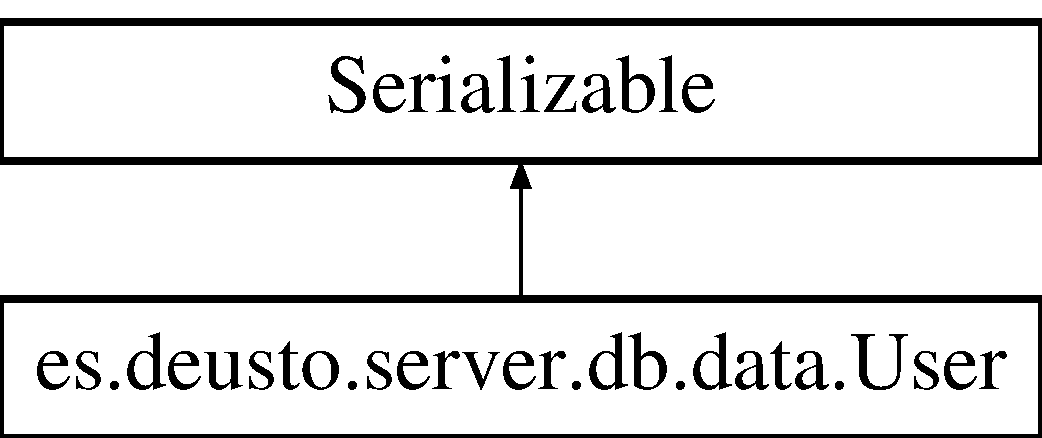
\includegraphics[height=2.000000cm]{classes_1_1deusto_1_1server_1_1db_1_1data_1_1_user}
\end{center}
\end{figure}
\subsection*{Public Member Functions}
\begin{DoxyCompactItemize}
\item 
\hyperlink{classes_1_1deusto_1_1server_1_1db_1_1data_1_1_user_accf4cd75adc5bfc6cd376a1714517ba9}{User} (String login, String password)
\item 
void \hyperlink{classes_1_1deusto_1_1server_1_1db_1_1data_1_1_user_a0fbb3860281941edb6832d0424910cd7}{add\+Money} (int money)
\item 
void \hyperlink{classes_1_1deusto_1_1server_1_1db_1_1data_1_1_user_a9de251663e6c2ecfdc5dcdac19224a1e}{remove\+Money} (int money)
\item 
String \hyperlink{classes_1_1deusto_1_1server_1_1db_1_1data_1_1_user_a2bc07e76806b027ef70b5ad8cea5f9fa}{get\+Login} ()
\item 
String \hyperlink{classes_1_1deusto_1_1server_1_1db_1_1data_1_1_user_ac576607b3eae9e9b8c7002d5cd7c1a62}{get\+Password} ()
\item 
void \hyperlink{classes_1_1deusto_1_1server_1_1db_1_1data_1_1_user_a0098f77da63338c8374ea1e5baab28c9}{set\+Password} (String password)
\item 
void \hyperlink{classes_1_1deusto_1_1server_1_1db_1_1data_1_1_user_a0e2c3f3fea559e9ab7eaab197fe9e015}{set\+Super} (boolean superU)
\item 
boolean \hyperlink{classes_1_1deusto_1_1server_1_1db_1_1data_1_1_user_a9f13d80d62b561e4fc76286cccf3333a}{get\+Super} ()
\item 
int \hyperlink{classes_1_1deusto_1_1server_1_1db_1_1data_1_1_user_a685ffb55326ae540eeb26eff13685a76}{get\+Money} ()
\item 
void \hyperlink{classes_1_1deusto_1_1server_1_1db_1_1data_1_1_user_af4381bf3a6dedebc28c50812cb71599a}{set\+Amount} (int number)
\item 
String \hyperlink{classes_1_1deusto_1_1server_1_1db_1_1data_1_1_user_a494980951c4c71c0a793994b7bcd5101}{to\+String} ()
\end{DoxyCompactItemize}


\subsection{Detailed Description}


Definition at line 17 of file User.\+java.



\subsection{Constructor \& Destructor Documentation}
\mbox{\Hypertarget{classes_1_1deusto_1_1server_1_1db_1_1data_1_1_user_accf4cd75adc5bfc6cd376a1714517ba9}\label{classes_1_1deusto_1_1server_1_1db_1_1data_1_1_user_accf4cd75adc5bfc6cd376a1714517ba9}} 
\index{es\+::deusto\+::server\+::db\+::data\+::\+User@{es\+::deusto\+::server\+::db\+::data\+::\+User}!User@{User}}
\index{User@{User}!es\+::deusto\+::server\+::db\+::data\+::\+User@{es\+::deusto\+::server\+::db\+::data\+::\+User}}
\subsubsection{\texorpdfstring{User()}{User()}}
{\footnotesize\ttfamily es.\+deusto.\+server.\+db.\+data.\+User.\+User (\begin{DoxyParamCaption}\item[{String}]{login,  }\item[{String}]{password }\end{DoxyParamCaption})}

Method to create a new instance of an object \hyperlink{classes_1_1deusto_1_1server_1_1db_1_1data_1_1_user}{User} 
\begin{DoxyParams}{Parameters}
{\em login} & The value for the PK that will identify a user between all the ones in the \hyperlink{classes_1_1deusto_1_1server_1_1db_1_1_d_b}{DB} \\
\hline
{\em password} & The value for the password of the user \\
\hline
\end{DoxyParams}


Definition at line 37 of file User.\+java.



\subsection{Member Function Documentation}
\mbox{\Hypertarget{classes_1_1deusto_1_1server_1_1db_1_1data_1_1_user_a0fbb3860281941edb6832d0424910cd7}\label{classes_1_1deusto_1_1server_1_1db_1_1data_1_1_user_a0fbb3860281941edb6832d0424910cd7}} 
\index{es\+::deusto\+::server\+::db\+::data\+::\+User@{es\+::deusto\+::server\+::db\+::data\+::\+User}!add\+Money@{add\+Money}}
\index{add\+Money@{add\+Money}!es\+::deusto\+::server\+::db\+::data\+::\+User@{es\+::deusto\+::server\+::db\+::data\+::\+User}}
\subsubsection{\texorpdfstring{add\+Money()}{addMoney()}}
{\footnotesize\ttfamily void es.\+deusto.\+server.\+db.\+data.\+User.\+add\+Money (\begin{DoxyParamCaption}\item[{int}]{money }\end{DoxyParamCaption})}

This method augments the value of the users amount of money for the parameter that is sent 
\begin{DoxyParams}{Parameters}
{\em money} & the amount of money to be added \\
\hline
\end{DoxyParams}


Definition at line 46 of file User.\+java.

\mbox{\Hypertarget{classes_1_1deusto_1_1server_1_1db_1_1data_1_1_user_a2bc07e76806b027ef70b5ad8cea5f9fa}\label{classes_1_1deusto_1_1server_1_1db_1_1data_1_1_user_a2bc07e76806b027ef70b5ad8cea5f9fa}} 
\index{es\+::deusto\+::server\+::db\+::data\+::\+User@{es\+::deusto\+::server\+::db\+::data\+::\+User}!get\+Login@{get\+Login}}
\index{get\+Login@{get\+Login}!es\+::deusto\+::server\+::db\+::data\+::\+User@{es\+::deusto\+::server\+::db\+::data\+::\+User}}
\subsubsection{\texorpdfstring{get\+Login()}{getLogin()}}
{\footnotesize\ttfamily String es.\+deusto.\+server.\+db.\+data.\+User.\+get\+Login (\begin{DoxyParamCaption}{ }\end{DoxyParamCaption})}

This method returns the PK of the user \begin{DoxyReturn}{Returns}
The username (login) of the user 
\end{DoxyReturn}


Definition at line 58 of file User.\+java.

\mbox{\Hypertarget{classes_1_1deusto_1_1server_1_1db_1_1data_1_1_user_a685ffb55326ae540eeb26eff13685a76}\label{classes_1_1deusto_1_1server_1_1db_1_1data_1_1_user_a685ffb55326ae540eeb26eff13685a76}} 
\index{es\+::deusto\+::server\+::db\+::data\+::\+User@{es\+::deusto\+::server\+::db\+::data\+::\+User}!get\+Money@{get\+Money}}
\index{get\+Money@{get\+Money}!es\+::deusto\+::server\+::db\+::data\+::\+User@{es\+::deusto\+::server\+::db\+::data\+::\+User}}
\subsubsection{\texorpdfstring{get\+Money()}{getMoney()}}
{\footnotesize\ttfamily int es.\+deusto.\+server.\+db.\+data.\+User.\+get\+Money (\begin{DoxyParamCaption}{ }\end{DoxyParamCaption})}

This method returns the amount of money of the user \begin{DoxyReturn}{Returns}
The amount value of the user 
\end{DoxyReturn}


Definition at line 96 of file User.\+java.

\mbox{\Hypertarget{classes_1_1deusto_1_1server_1_1db_1_1data_1_1_user_ac576607b3eae9e9b8c7002d5cd7c1a62}\label{classes_1_1deusto_1_1server_1_1db_1_1data_1_1_user_ac576607b3eae9e9b8c7002d5cd7c1a62}} 
\index{es\+::deusto\+::server\+::db\+::data\+::\+User@{es\+::deusto\+::server\+::db\+::data\+::\+User}!get\+Password@{get\+Password}}
\index{get\+Password@{get\+Password}!es\+::deusto\+::server\+::db\+::data\+::\+User@{es\+::deusto\+::server\+::db\+::data\+::\+User}}
\subsubsection{\texorpdfstring{get\+Password()}{getPassword()}}
{\footnotesize\ttfamily String es.\+deusto.\+server.\+db.\+data.\+User.\+get\+Password (\begin{DoxyParamCaption}{ }\end{DoxyParamCaption})}

This method returns the pass of the user \begin{DoxyReturn}{Returns}
The password of the user 
\end{DoxyReturn}


Definition at line 66 of file User.\+java.

\mbox{\Hypertarget{classes_1_1deusto_1_1server_1_1db_1_1data_1_1_user_a9f13d80d62b561e4fc76286cccf3333a}\label{classes_1_1deusto_1_1server_1_1db_1_1data_1_1_user_a9f13d80d62b561e4fc76286cccf3333a}} 
\index{es\+::deusto\+::server\+::db\+::data\+::\+User@{es\+::deusto\+::server\+::db\+::data\+::\+User}!get\+Super@{get\+Super}}
\index{get\+Super@{get\+Super}!es\+::deusto\+::server\+::db\+::data\+::\+User@{es\+::deusto\+::server\+::db\+::data\+::\+User}}
\subsubsection{\texorpdfstring{get\+Super()}{getSuper()}}
{\footnotesize\ttfamily boolean es.\+deusto.\+server.\+db.\+data.\+User.\+get\+Super (\begin{DoxyParamCaption}{ }\end{DoxyParamCaption})}

This method returns the superU value of the user \begin{DoxyReturn}{Returns}
The superU value of the user 
\end{DoxyReturn}


Definition at line 90 of file User.\+java.

\mbox{\Hypertarget{classes_1_1deusto_1_1server_1_1db_1_1data_1_1_user_a9de251663e6c2ecfdc5dcdac19224a1e}\label{classes_1_1deusto_1_1server_1_1db_1_1data_1_1_user_a9de251663e6c2ecfdc5dcdac19224a1e}} 
\index{es\+::deusto\+::server\+::db\+::data\+::\+User@{es\+::deusto\+::server\+::db\+::data\+::\+User}!remove\+Money@{remove\+Money}}
\index{remove\+Money@{remove\+Money}!es\+::deusto\+::server\+::db\+::data\+::\+User@{es\+::deusto\+::server\+::db\+::data\+::\+User}}
\subsubsection{\texorpdfstring{remove\+Money()}{removeMoney()}}
{\footnotesize\ttfamily void es.\+deusto.\+server.\+db.\+data.\+User.\+remove\+Money (\begin{DoxyParamCaption}\item[{int}]{money }\end{DoxyParamCaption})}

This method reduces the value of the users amount of money for the parameter that is sent 
\begin{DoxyParams}{Parameters}
{\em money} & the amount of money to be removed \\
\hline
\end{DoxyParams}


Definition at line 52 of file User.\+java.

\mbox{\Hypertarget{classes_1_1deusto_1_1server_1_1db_1_1data_1_1_user_af4381bf3a6dedebc28c50812cb71599a}\label{classes_1_1deusto_1_1server_1_1db_1_1data_1_1_user_af4381bf3a6dedebc28c50812cb71599a}} 
\index{es\+::deusto\+::server\+::db\+::data\+::\+User@{es\+::deusto\+::server\+::db\+::data\+::\+User}!set\+Amount@{set\+Amount}}
\index{set\+Amount@{set\+Amount}!es\+::deusto\+::server\+::db\+::data\+::\+User@{es\+::deusto\+::server\+::db\+::data\+::\+User}}
\subsubsection{\texorpdfstring{set\+Amount()}{setAmount()}}
{\footnotesize\ttfamily void es.\+deusto.\+server.\+db.\+data.\+User.\+set\+Amount (\begin{DoxyParamCaption}\item[{int}]{number }\end{DoxyParamCaption})}

Establishes the value for the parameter amount of the user 
\begin{DoxyParams}{Parameters}
{\em amount} & The value of the users amount parameter \\
\hline
\end{DoxyParams}


Definition at line 102 of file User.\+java.

\mbox{\Hypertarget{classes_1_1deusto_1_1server_1_1db_1_1data_1_1_user_a0098f77da63338c8374ea1e5baab28c9}\label{classes_1_1deusto_1_1server_1_1db_1_1data_1_1_user_a0098f77da63338c8374ea1e5baab28c9}} 
\index{es\+::deusto\+::server\+::db\+::data\+::\+User@{es\+::deusto\+::server\+::db\+::data\+::\+User}!set\+Password@{set\+Password}}
\index{set\+Password@{set\+Password}!es\+::deusto\+::server\+::db\+::data\+::\+User@{es\+::deusto\+::server\+::db\+::data\+::\+User}}
\subsubsection{\texorpdfstring{set\+Password()}{setPassword()}}
{\footnotesize\ttfamily void es.\+deusto.\+server.\+db.\+data.\+User.\+set\+Password (\begin{DoxyParamCaption}\item[{String}]{password }\end{DoxyParamCaption})}

Establishes the value for the parameter password of the user 
\begin{DoxyParams}{Parameters}
{\em password} & The value for the new password \\
\hline
\end{DoxyParams}


Definition at line 74 of file User.\+java.

\mbox{\Hypertarget{classes_1_1deusto_1_1server_1_1db_1_1data_1_1_user_a0e2c3f3fea559e9ab7eaab197fe9e015}\label{classes_1_1deusto_1_1server_1_1db_1_1data_1_1_user_a0e2c3f3fea559e9ab7eaab197fe9e015}} 
\index{es\+::deusto\+::server\+::db\+::data\+::\+User@{es\+::deusto\+::server\+::db\+::data\+::\+User}!set\+Super@{set\+Super}}
\index{set\+Super@{set\+Super}!es\+::deusto\+::server\+::db\+::data\+::\+User@{es\+::deusto\+::server\+::db\+::data\+::\+User}}
\subsubsection{\texorpdfstring{set\+Super()}{setSuper()}}
{\footnotesize\ttfamily void es.\+deusto.\+server.\+db.\+data.\+User.\+set\+Super (\begin{DoxyParamCaption}\item[{boolean}]{superU }\end{DoxyParamCaption})}

Establishes the value for the parameter superU of the user 
\begin{DoxyParams}{Parameters}
{\em superU} & The value of the users superU parameter \\
\hline
\end{DoxyParams}


Definition at line 82 of file User.\+java.

\mbox{\Hypertarget{classes_1_1deusto_1_1server_1_1db_1_1data_1_1_user_a494980951c4c71c0a793994b7bcd5101}\label{classes_1_1deusto_1_1server_1_1db_1_1data_1_1_user_a494980951c4c71c0a793994b7bcd5101}} 
\index{es\+::deusto\+::server\+::db\+::data\+::\+User@{es\+::deusto\+::server\+::db\+::data\+::\+User}!to\+String@{to\+String}}
\index{to\+String@{to\+String}!es\+::deusto\+::server\+::db\+::data\+::\+User@{es\+::deusto\+::server\+::db\+::data\+::\+User}}
\subsubsection{\texorpdfstring{to\+String()}{toString()}}
{\footnotesize\ttfamily String es.\+deusto.\+server.\+db.\+data.\+User.\+to\+String (\begin{DoxyParamCaption}{ }\end{DoxyParamCaption})}



Definition at line 104 of file User.\+java.



The documentation for this class was generated from the following file\+:\begin{DoxyCompactItemize}
\item 
C\+:/\+Users/\+Oihane/git/\+S\+P\+Q03/spq03/src/main/java/es/deusto/server/db/data/\hyperlink{_user_8java}{User.\+java}\end{DoxyCompactItemize}

\chapter{File Documentation}
\hypertarget{_client_8java}{}\section{C\+:/\+Users/\+Oihane/git/\+S\+P\+Q03/spq03/src/main/java/es/deusto/client/\+Client.java File Reference}
\label{_client_8java}\index{C\+:/\+Users/\+Oihane/git/\+S\+P\+Q03/spq03/src/main/java/es/deusto/client/\+Client.\+java@{C\+:/\+Users/\+Oihane/git/\+S\+P\+Q03/spq03/src/main/java/es/deusto/client/\+Client.\+java}}
\subsection*{Classes}
\begin{DoxyCompactItemize}
\item 
class \hyperlink{classes_1_1deusto_1_1client_1_1_client}{es.\+deusto.\+client.\+Client}
\end{DoxyCompactItemize}
\subsection*{Packages}
\begin{DoxyCompactItemize}
\item 
package \hyperlink{namespacees_1_1deusto_1_1client}{es.\+deusto.\+client}
\end{DoxyCompactItemize}

\hypertarget{_new_prod_window_8java}{}\section{C\+:/\+Users/\+Oihane/git/\+S\+P\+Q03/spq03/src/main/java/es/deusto/client/\+New\+Prod\+Window.java File Reference}
\label{_new_prod_window_8java}\index{C\+:/\+Users/\+Oihane/git/\+S\+P\+Q03/spq03/src/main/java/es/deusto/client/\+New\+Prod\+Window.\+java@{C\+:/\+Users/\+Oihane/git/\+S\+P\+Q03/spq03/src/main/java/es/deusto/client/\+New\+Prod\+Window.\+java}}
\subsection*{Classes}
\begin{DoxyCompactItemize}
\item 
class \hyperlink{classes_1_1deusto_1_1client_1_1_new_prod_window}{es.\+deusto.\+client.\+New\+Prod\+Window}
\end{DoxyCompactItemize}
\subsection*{Packages}
\begin{DoxyCompactItemize}
\item 
package \hyperlink{namespacees_1_1deusto_1_1client}{es.\+deusto.\+client}
\end{DoxyCompactItemize}

\hypertarget{_d_a_o_8java}{}\section{C\+:/\+Users/\+Oihane/git/\+S\+P\+Q03/spq03/src/main/java/es/deusto/server/db/dao/\+D\+AO.java File Reference}
\label{_d_a_o_8java}\index{C\+:/\+Users/\+Oihane/git/\+S\+P\+Q03/spq03/src/main/java/es/deusto/server/db/dao/\+D\+A\+O.\+java@{C\+:/\+Users/\+Oihane/git/\+S\+P\+Q03/spq03/src/main/java/es/deusto/server/db/dao/\+D\+A\+O.\+java}}
\subsection*{Classes}
\begin{DoxyCompactItemize}
\item 
class \hyperlink{classes_1_1deusto_1_1server_1_1db_1_1dao_1_1_d_a_o}{es.\+deusto.\+server.\+db.\+dao.\+D\+AO}
\end{DoxyCompactItemize}
\subsection*{Packages}
\begin{DoxyCompactItemize}
\item 
package \hyperlink{namespacees_1_1deusto_1_1server_1_1db_1_1dao}{es.\+deusto.\+server.\+db.\+dao}
\end{DoxyCompactItemize}

\hypertarget{_i_d_a_o_8java}{}\section{C\+:/\+Users/\+Oihane/git/\+S\+P\+Q03/spq03/src/main/java/es/deusto/server/db/dao/\+I\+D\+AO.java File Reference}
\label{_i_d_a_o_8java}\index{C\+:/\+Users/\+Oihane/git/\+S\+P\+Q03/spq03/src/main/java/es/deusto/server/db/dao/\+I\+D\+A\+O.\+java@{C\+:/\+Users/\+Oihane/git/\+S\+P\+Q03/spq03/src/main/java/es/deusto/server/db/dao/\+I\+D\+A\+O.\+java}}
\subsection*{Classes}
\begin{DoxyCompactItemize}
\item 
interface \hyperlink{interfacees_1_1deusto_1_1server_1_1db_1_1dao_1_1_i_d_a_o}{es.\+deusto.\+server.\+db.\+dao.\+I\+D\+AO}
\end{DoxyCompactItemize}
\subsection*{Packages}
\begin{DoxyCompactItemize}
\item 
package \hyperlink{namespacees_1_1deusto_1_1server_1_1db_1_1dao}{es.\+deusto.\+server.\+db.\+dao}
\end{DoxyCompactItemize}

\hypertarget{_money_8java}{}\section{C\+:/\+Users/\+Oihane/git/\+S\+P\+Q03/spq03/src/main/java/es/deusto/server/db/data/\+Money.java File Reference}
\label{_money_8java}\index{C\+:/\+Users/\+Oihane/git/\+S\+P\+Q03/spq03/src/main/java/es/deusto/server/db/data/\+Money.\+java@{C\+:/\+Users/\+Oihane/git/\+S\+P\+Q03/spq03/src/main/java/es/deusto/server/db/data/\+Money.\+java}}
\subsection*{Classes}
\begin{DoxyCompactItemize}
\item 
class \hyperlink{classes_1_1deusto_1_1server_1_1db_1_1data_1_1_money}{es.\+deusto.\+server.\+db.\+data.\+Money}
\end{DoxyCompactItemize}
\subsection*{Packages}
\begin{DoxyCompactItemize}
\item 
package \hyperlink{namespacees_1_1deusto_1_1server_1_1db_1_1data}{es.\+deusto.\+server.\+db.\+data}
\end{DoxyCompactItemize}

\hypertarget{_product_8java}{}\section{C\+:/\+Users/\+Oihane/git/\+S\+P\+Q03/spq03/src/main/java/es/deusto/server/db/data/\+Product.java File Reference}
\label{_product_8java}\index{C\+:/\+Users/\+Oihane/git/\+S\+P\+Q03/spq03/src/main/java/es/deusto/server/db/data/\+Product.\+java@{C\+:/\+Users/\+Oihane/git/\+S\+P\+Q03/spq03/src/main/java/es/deusto/server/db/data/\+Product.\+java}}
\subsection*{Classes}
\begin{DoxyCompactItemize}
\item 
class \hyperlink{classes_1_1deusto_1_1server_1_1db_1_1data_1_1_product}{es.\+deusto.\+server.\+db.\+data.\+Product}
\end{DoxyCompactItemize}
\subsection*{Packages}
\begin{DoxyCompactItemize}
\item 
package \hyperlink{namespacees_1_1deusto_1_1server_1_1db_1_1data}{es.\+deusto.\+server.\+db.\+data}
\end{DoxyCompactItemize}

\hypertarget{_user_8java}{}\section{C\+:/\+Users/\+Oihane/git/\+S\+P\+Q03/spq03/src/main/java/es/deusto/server/db/data/\+User.java File Reference}
\label{_user_8java}\index{C\+:/\+Users/\+Oihane/git/\+S\+P\+Q03/spq03/src/main/java/es/deusto/server/db/data/\+User.\+java@{C\+:/\+Users/\+Oihane/git/\+S\+P\+Q03/spq03/src/main/java/es/deusto/server/db/data/\+User.\+java}}
\subsection*{Classes}
\begin{DoxyCompactItemize}
\item 
class \hyperlink{classes_1_1deusto_1_1server_1_1db_1_1data_1_1_user}{es.\+deusto.\+server.\+db.\+data.\+User}
\end{DoxyCompactItemize}
\subsection*{Packages}
\begin{DoxyCompactItemize}
\item 
package \hyperlink{namespacees_1_1deusto_1_1server_1_1db_1_1data}{es.\+deusto.\+server.\+db.\+data}
\end{DoxyCompactItemize}

\hypertarget{_d_b_8java}{}\section{C\+:/\+Users/\+Oihane/git/\+S\+P\+Q03/spq03/src/main/java/es/deusto/server/db/\+DB.java File Reference}
\label{_d_b_8java}\index{C\+:/\+Users/\+Oihane/git/\+S\+P\+Q03/spq03/src/main/java/es/deusto/server/db/\+D\+B.\+java@{C\+:/\+Users/\+Oihane/git/\+S\+P\+Q03/spq03/src/main/java/es/deusto/server/db/\+D\+B.\+java}}
\subsection*{Classes}
\begin{DoxyCompactItemize}
\item 
class \hyperlink{classes_1_1deusto_1_1server_1_1db_1_1_d_b}{es.\+deusto.\+server.\+db.\+DB}
\end{DoxyCompactItemize}
\subsection*{Packages}
\begin{DoxyCompactItemize}
\item 
package \hyperlink{namespacees_1_1deusto_1_1server_1_1db}{es.\+deusto.\+server.\+db}
\end{DoxyCompactItemize}

\hypertarget{_i_d_b_8java}{}\section{C\+:/\+Users/\+Oihane/git/\+S\+P\+Q03/spq03/src/main/java/es/deusto/server/db/\+I\+DB.java File Reference}
\label{_i_d_b_8java}\index{C\+:/\+Users/\+Oihane/git/\+S\+P\+Q03/spq03/src/main/java/es/deusto/server/db/\+I\+D\+B.\+java@{C\+:/\+Users/\+Oihane/git/\+S\+P\+Q03/spq03/src/main/java/es/deusto/server/db/\+I\+D\+B.\+java}}
\subsection*{Classes}
\begin{DoxyCompactItemize}
\item 
interface \hyperlink{interfacees_1_1deusto_1_1server_1_1db_1_1_i_d_b}{es.\+deusto.\+server.\+db.\+I\+DB}
\end{DoxyCompactItemize}
\subsection*{Packages}
\begin{DoxyCompactItemize}
\item 
package \hyperlink{namespacees_1_1deusto_1_1server_1_1db}{es.\+deusto.\+server.\+db}
\end{DoxyCompactItemize}

\hypertarget{_i_transferer_8java}{}\section{C\+:/\+Users/\+Oihane/git/\+S\+P\+Q03/spq03/src/main/java/es/deusto/server/remote/\+I\+Transferer.java File Reference}
\label{_i_transferer_8java}\index{C\+:/\+Users/\+Oihane/git/\+S\+P\+Q03/spq03/src/main/java/es/deusto/server/remote/\+I\+Transferer.\+java@{C\+:/\+Users/\+Oihane/git/\+S\+P\+Q03/spq03/src/main/java/es/deusto/server/remote/\+I\+Transferer.\+java}}
\subsection*{Classes}
\begin{DoxyCompactItemize}
\item 
interface \hyperlink{interfacees_1_1deusto_1_1server_1_1remote_1_1_i_transferer}{es.\+deusto.\+server.\+remote.\+I\+Transferer}
\end{DoxyCompactItemize}
\subsection*{Packages}
\begin{DoxyCompactItemize}
\item 
package \hyperlink{namespacees_1_1deusto_1_1server_1_1remote}{es.\+deusto.\+server.\+remote}
\end{DoxyCompactItemize}

\hypertarget{_transferer_8java}{}\section{C\+:/\+Users/\+Oihane/git/\+S\+P\+Q03/spq03/src/main/java/es/deusto/server/remote/\+Transferer.java File Reference}
\label{_transferer_8java}\index{C\+:/\+Users/\+Oihane/git/\+S\+P\+Q03/spq03/src/main/java/es/deusto/server/remote/\+Transferer.\+java@{C\+:/\+Users/\+Oihane/git/\+S\+P\+Q03/spq03/src/main/java/es/deusto/server/remote/\+Transferer.\+java}}
\subsection*{Classes}
\begin{DoxyCompactItemize}
\item 
class \hyperlink{classes_1_1deusto_1_1server_1_1remote_1_1_transferer}{es.\+deusto.\+server.\+remote.\+Transferer}
\end{DoxyCompactItemize}
\subsection*{Packages}
\begin{DoxyCompactItemize}
\item 
package \hyperlink{namespacees_1_1deusto_1_1server_1_1remote}{es.\+deusto.\+server.\+remote}
\end{DoxyCompactItemize}

\hypertarget{_server_8java}{}\section{C\+:/\+Users/\+Oihane/git/\+S\+P\+Q03/spq03/src/main/java/es/deusto/server/\+Server.java File Reference}
\label{_server_8java}\index{C\+:/\+Users/\+Oihane/git/\+S\+P\+Q03/spq03/src/main/java/es/deusto/server/\+Server.\+java@{C\+:/\+Users/\+Oihane/git/\+S\+P\+Q03/spq03/src/main/java/es/deusto/server/\+Server.\+java}}
\subsection*{Classes}
\begin{DoxyCompactItemize}
\item 
class \hyperlink{classes_1_1deusto_1_1server_1_1_server}{es.\+deusto.\+server.\+Server}
\end{DoxyCompactItemize}
\subsection*{Packages}
\begin{DoxyCompactItemize}
\item 
package \hyperlink{namespacees_1_1deusto_1_1server}{es.\+deusto.\+server}
\end{DoxyCompactItemize}

\hypertarget{_j_unit_test_8java}{}\section{C\+:/\+Users/\+Oihane/git/\+S\+P\+Q03/spq03/src/test/java/es/deusto/server/\+J\+Unit\+Test.java File Reference}
\label{_j_unit_test_8java}\index{C\+:/\+Users/\+Oihane/git/\+S\+P\+Q03/spq03/src/test/java/es/deusto/server/\+J\+Unit\+Test.\+java@{C\+:/\+Users/\+Oihane/git/\+S\+P\+Q03/spq03/src/test/java/es/deusto/server/\+J\+Unit\+Test.\+java}}
\subsection*{Classes}
\begin{DoxyCompactItemize}
\item 
class \hyperlink{classes_1_1deusto_1_1server_1_1_j_unit_test}{es.\+deusto.\+server.\+J\+Unit\+Test}
\end{DoxyCompactItemize}
\subsection*{Packages}
\begin{DoxyCompactItemize}
\item 
package \hyperlink{namespacees_1_1deusto_1_1server}{es.\+deusto.\+server}
\end{DoxyCompactItemize}

%--- End generated contents ---

% Index
\backmatter
\newpage
\phantomsection
\clearemptydoublepage
\addcontentsline{toc}{chapter}{Index}
\printindex

\end{document}
